\DIFaddbegin \chapter{\label{ch:trigg}\DIFadd{UPC Trigger development for CMS}}
  \DIFadd{Rare physics process at the LHC require dedicated triggers in order to sort
    these processes from the billions of ordinary nucleus-nucleus collisions. 
  Unlike most heavy-ion triggers, UPC triggers are optimized for low-}\pt{} 
    \DIFadd{and low multiplicity events. 
  For this reason trigger development specific to UPC events was required to
    carry out the analysis in this thesis.
}

  \DIFadd{The increase in collision rate of the LHC PbPb beams from 2010 to 2011 was
    nearly a factor of 15. 
  To accommodate this increase in rate, the 2011 trigger scheme needed to be 
    more selective than in 2010 where CMS could take any event which 
    appeared to have a collision.
  The available bandwidth was allocated equally amongst the various heavy ion
    analysis groups to pursue as wide a physics program as possible.
  From this consideration, bandwidth limits were placed on the trigger rates
    for each analysis group's trigger package. 
  }

  \section{\label{sec:l1Trigger}\DIFadd{L1 trigger}}
    \DIFadd{The UPC L1 triggers were designed to study UPC }\JPsi{} \DIFadd{production via the 
      dimuon and dielectron channels (see Section~\ref{sec:detTrg}).
    To achieve this, the loosest muon and electron triggers where combined with
      a trigger on energy in the ZDCs and no activity in BSCs (BSC veto).
    Additional triggers were commissioned in case radiation damage during the 
      run reduced the sensitivity of the BSCs.
    This required no activity in HF (HF veto). 
    These triggers are summarized in Table~\ref{tab:l1Triggers2011}.
    The ECAL2 and ECAL5 triggers in Table~\ref{tab:l1Triggers2011}
      indicate a 5 and 2 GeV threshold on $E_{T}$ measured in the ECAL.
    The MuonOpen trigger indicates that the trigger only 
      requires a muon candidate in one of the three muon sub-systems and that
      there is no momentum threshold.
    ZDC in the trigger names indicate energy constant with at least one neutron.
    The sign on the ZDC label indicates which of the two ZDCs is required. 
}

    \begin{table}[h]
      \centering
      \begin{tabular}{|l|l|l|l|l|}
        \hline \DIFaddFL{L1 trigger name }& \DIFaddFL{Rate (Hz) }& \DIFaddFL{Prescale }& \DIFaddFL{Id }& \DIFaddFL{Type }\\ \hline \hline
        \DIFaddFL{MuonOpen and (ZDC$^{+}$~or~ZDC$^{-}$) and BSC veto }& \DIFaddFL{2.1 }& \DIFaddFL{1 }& \DIFaddFL{1 }& \multirow{3}{*}{Physics} \\  \hhline{----~}
        \DIFaddFL{ECAL2 and (ZDC$^{+}$~or~ZDC$^{-}$) and BSC veto }& \DIFaddFL{1.8 }& \DIFaddFL{2 }& \DIFaddFL{2 }& \\  \hhline{----~}
        \DIFaddFL{ECAL5 and (ZDC$^{+}$~or~ZDC$^{-}$) and BSC veto }& \DIFaddFL{0.3 }& \DIFaddFL{1 }& \DIFaddFL{3 }& \\  \hline
        \DIFaddFL{(ZDC$^{+}$~or~ZDC$^{-}$) }& \DIFaddFL{35 }& \DIFaddFL{1500 }& \DIFaddFL{4 }& \DIFaddFL{Monitor }\\  \hline
        \DIFaddFL{MuonOpen and (ZDC$^{+}$~or~ZDC$^{-}$) and HF veto }& \DIFaddFL{0 }& \DIFaddFL{off }& \DIFaddFL{5 }& \multirow{3}{*}{Backup} \\ \hhline{----~}
        \DIFaddFL{ECAL2 and (ZDC$^{+}$~or~ZDC$^{-}$) and HF veto }& \DIFaddFL{0 }& \DIFaddFL{off }& \DIFaddFL{6 }& \\  \hhline{----~}
        \DIFaddFL{ECAL5 and (ZDC$^{+}$~or~ZDC$^{-}$) and HF veto }& \DIFaddFL{0 }& \DIFaddFL{off }& \DIFaddFL{7 }& \\  \hline
      \end{tabular}
      \caption{\DIFaddFL{List of 2011 L1 seeds.}}
      \label{tab:l1Triggers2011}
    \end{table}
    \DIFadd{The cumulative L1 trigger rate for all the UPC L1 trigger seeds was
      required to be no greater than 200 Hz.
    This requirement comes from the need to keep the tracker read-out rate
      low. 
    The trackers baseline voltage can fluctuate due to the high tracker hit 
      multiplicities in PbPb collisions.
    In order to monitor the zero suppression of the tracker, the zero 
      suppression algorithm was executed using the HLT computing farm 
	      rather than in the tracker firmware.
}

    \DIFadd{In order to record the efficiency monitoring data, the ZDC triggers were
      reduce to a lower rate by only keeping a fraction of the total trigger 
      rate. 
    The factor that the trigger rate is reduced by is called the prescale.
    A prescale of 2 for example means that half the triggers that were 
      accepted.
    If the prescale is set to 1, then whole trigger rate is accepted. 
    The prescales for the triggers were set to balance the competing objectives 
      of rate reduction and increasing the overlap between the monitoring and
      signal triggers.
}

  \section{\label{sec:hltTrigger}\DIFadd{HLT trigger}}
    \DIFadd{An event must pass the selection criteria of an HLT path in order to be
      recorded. 
    As opposed to the L1 trigger, which has access only to information from
      calorimeters and muon chambers, the HLT has access to all of the CMS 
      sub-detectors including the tracker. 
    Reconstruction of a track in the pixel detector is used by the UPC 
      trigger paths.
    The use of the pixel detector only, as opposed to using the whole tracker 
      including the silicon strip detector, allows for quick track 
      reconstruction saving computing cycles.
    The UPC triggers were required to have at lease one reconstructed pixel 
      track in order to reject backgrounds where no particles are 
      reconstructed by the tracker.
    For the muon trigger in Table~\ref{tab:hltTriggers2011} the rate was 
      reduced by nearly a factor or 4 compared to its L1 seed rate in 
      Table~\ref{tab:l1Triggers2011}.
    }\begin{table}[h]
      \centering
      \begin{tabular}{|l|l|l|l|l|l|}
        \hline \DIFaddFL{HLT trigger  }& \DIFaddFL{Rate (Hz) }& \DIFaddFL{L1 prescale }& \DIFaddFL{HLT prescale }& \DIFaddFL{L1 seed }& \DIFaddFL{Type }\\ \hline \hline
        \DIFaddFL{L1UPCMuon and Pixel Track }& \DIFaddFL{0.52 }& \DIFaddFL{1 }& \DIFaddFL{1 }& \DIFaddFL{1 }& \multirow{3}{*}{Physics} \\ \hhline{-----~} 
        \DIFaddFL{L1UPCECAL2 and Pixel Track }& \DIFaddFL{1.65 }& \DIFaddFL{2 }& \DIFaddFL{1 }& \DIFaddFL{2 }& \\ \hhline{-----~}
        \DIFaddFL{L1UPCECAL5 and Pixel Track }& \DIFaddFL{0.26 }& \DIFaddFL{1 }& \DIFaddFL{1 }& \DIFaddFL{3 }& \\ \hline
        \DIFaddFL{L1ZDCOr }& \DIFaddFL{3.6 }& \DIFaddFL{1500 }& \DIFaddFL{11 }& \DIFaddFL{4 }& \multirow{2}{*}{Monitor}  \\ \hhline{-----~}
        \DIFaddFL{L1ZDCOr and Pixel Track }& \DIFaddFL{2.8 }& \DIFaddFL{1500 }& \DIFaddFL{1 }& \DIFaddFL{4 }& \\ \hline
        \DIFaddFL{L1UPCMuonHFVeto and Pixel Track }& \DIFaddFL{0 }& \DIFaddFL{off }& \DIFaddFL{off }& \DIFaddFL{5 }& \multirow{3}{*}{Backup}   \\ \hhline{-----~}
        \DIFaddFL{L1UPCECAL2HFVeto and Pixel Track }& \DIFaddFL{0 }& \DIFaddFL{off }& \DIFaddFL{off }& \DIFaddFL{6 }& \\ \hhline{-----~}
        \DIFaddFL{L1UPCECAL5HFVeto and Pixel Track }& \DIFaddFL{0 }& \DIFaddFL{off }& \DIFaddFL{off }& \DIFaddFL{7 }& \\ \hline 
      \end{tabular}
      \caption{\DIFaddFL{List of 2011 HLT trigger.}}
      \label{tab:hltTriggers2011}
    \end{table}

    \DIFadd{The total HLT output for the UPC trigger package was limited to 20 Hz. 
    The limiting factor for the HLT rate was the amount of disk space given 
      to this analysis. 
    To meet the bandwidth requirements and collect a significant sample
      of data for estimating efficiencies, the prescales were balanced with 
      the goal of achieving at least 5\% statistical precision on the 
      efficiency measurements. 
    As an example of the balancing of the prescales, the HLT  ZDC trigger that 
      did not require a pixel track was given a additional prescale factor 
      of 11 on the HLT.
    The ZDC path that also required a pixel track on the HLT, which used 
      the same L1 seed, was only prescaled at the L1.
    The prescale of 11 was set to ensure that at least 1000 of the pixel track 
      ZDC triggers overlapped with the ZDC L1 only triggers so that efficiency
      of the pixel track requirement in the trigger could be estimated from 
      the tracks lost.
}

 \section{\label{sec:pPbTrigDev}\DIFadd{Trigger development for the LHC pPb Run}}
   \DIFadd{Specific UPC triggers were also developed for the pPb run in 2013. 
    For this period of running a much higher total trigger rate was read out 
      relative to 2011.
    The total rate allocated for UPC triggers at the L1 in 2013 was 5 kHz and 
      50 Hz at the HLT.
    This factor of 5 increase in HLT and factor of 25 in L1 bandwidth,
      allowed for a change in emphasis from the L1 to the HLT. 
}

    \DIFadd{The basic strategy in 2013 was the same as in 2012, use the loosest 
      available ECAL and muon L1 triggers to push to capture the lowest }\pt{}
      \DIFadd{electrons and muons possible and reject hadronic interactions.
    Because of the L1 bandwidth restrictions in 2011, both the ZDCs and the 
      BCSs were used on the L1 to reduce rates.
    In 2013 only the muon and ECAL triggers were used on the L1 allowing for 
      rejection of hadronic interactions through cuts on track multiplicity. 
    In addition, a more sophisticated trigger using full dimuon reconstructed 
      was developed to increase purity.
    The main advantage in this shift in strategy was a higher purity due to 
      the increased sophistication of the reconstruction on the HLT.
    In addition, an increase in cross section of the underlying physics process
      was achieved by relaxing the neutron emission requirement.
}

    \DIFadd{The HLT triggers in 2013 rejected hadronic interactions through counting
      tracks. 
    For the five UPC trigger paths included in the HLT menu, 
      three levels of reconstruction were done at the HLT.
}

    \begin{itemize}
      \item \DIFadd{Pixel tracks were reconstructed from the inner pixel section of the 
        silicone tracker alone, tracks were reconstructed using the full
        tracker using the strips as well, and full dimuon reconstruction was 
        done using the tracker and muon detector. 
      }\item \DIFadd{The least restrictive pixel track paths required at least 
        one track reconstructed from the pixel detector and less than 10 pixel 
        tracks in the event.
      }\item \DIFadd{Full tracking paths were added on top of the pixel track paths and included
        an additional requirement of one full track and less than 7 reconstructed
        tracks.
      }\item \DIFadd{The most restrictive path added to the pixel and full tracking paths and 
        required reconstruction of dimuons with a mass between 2 and 12 GeV.
    }\end{itemize}


\DIFaddend \chapter{\label{ch:analysis} Analysis}
  In this chapter the various parts of the analysis are explained. 
  In Section~\ref{sec:mcSim}, the simulations used to estimate the detector's 
    ability to measure UPC processes are discussed. 
  \DIFdelbegin \DIFdel{Section~\ref{sec:TrigDev} explains the considerations that went into the 
    triggers that were developed for this measurement.
  }\DIFdelend The selection of UPC events is detailed in Section~\ref{sec:DataSetEvSel}.
  Extraction of the number of coherent \JPsi{} candidates is explained in 
    Section~\ref{sec:sigEx}.
  The determination of the detector's efficiency for measuring UPC events is 
    explained in Section~\ref{sec:effDet}.
  Finally, Section~\ref{sec:sysCheck} lays out the systematic uncertainties 
    for the measurement. 

  \section{\label{sec:mcSim} Physics generators and Monte Carlo simulations}
    Every physical measurement is the product of the underlying physics 
      folded with the response of the detector used to do the measurement. 
    In order to understand the underlying physical process, the detector's 
      effect on the measurement must be understood and accounted for. 
    As instruments become more and more complicated, the interplay among all
      of the many parts of the detector makes an analytic approach to the 
      problem untenable.
    For this reason, the numerical technique of Monte Carlo (MC) simulation is
      often the most effective approach for describing detector effects.

    MC simulations use random number generation to model the many statistical 
      effects of particles interacting with different parts of the detector. 
    First, particles are generated according to theoretical distributions.
    These particles are then propagated through a simulation of the detector.
    As the particles pass through the detector, random numbers are used
      to determine how these particles interact with the materials of the 
      detector based on the known properties of the material. 
    In this way, the theoretical distributions are convolved with a realistic 
      model of the detector's response. 
    A more detailed picture of how the detector shapes the underlaying 
      distributions emerges with each successive event.
    The final goal of the MC simulation is to produce a set of events that 
      accurately reproduce what would be measured if the theoretical input 
      describes nature well. 

  \subsection{STARlight and particle gun MC in CMS}
    In this thesis, two classes of generator input samples were used, 
      STARlight \DIFaddbegin \DIFadd{\mbox{%DIFAUXCMD
\cite{vmd1999 , starlight}
}%DIFAUXCMD
}\DIFaddend and a particle gun.
    The STARlight samples \DIFdelbegin \DIFdel{corresponds }\DIFdelend \DIFaddbegin \DIFadd{correspond }\DIFaddend to the theoretical calculations 
      described in Section~\ref{sec:vdmTheory}, while the particle gun produces
      particles with a user defined \DIFdelbegin \DIFdel{momentum distribution}\DIFdelend \DIFaddbegin \DIFadd{transverse momentum distribution and 
      rapidity distribution and isotropic decay to muon pairs in the }\JPsi{} 
      \DIFadd{rest frame}\DIFaddend . 
    For STARlight\DIFaddbegin \DIFadd{, }\DIFaddend three different physical process \DIFdelbegin \DIFdel{are simulated;
      }\DIFdelend \DIFaddbegin \DIFadd{were simulated:
      }\DIFaddend coherent \JPsi{} production, where the photon couples to the nucleus as
      a whole\DIFdelbegin \DIFdel{, }\DIFdelend \DIFaddbegin \DIFadd{; }\DIFaddend incoherent \JPsi{} production\DIFdelbegin \DIFdel{, }\DIFdelend \DIFaddbegin \DIFadd{; }\DIFaddend where the photon couples to a
      \DIFaddbegin \DIFadd{single }\DIFaddend nucleon within the nucleus, and photon-photon interactions, where 
      the photons from the two nuclei interact with each other to produce a 
      pair of oppositely charge muons\DIFdelbegin \DIFdel{directly}\DIFdelend .
    All three STARlight samples contain a $\mu^{+}$ and $\mu^{-}$ in the final 
      state.
\DIFdelbegin \DIFdel{The second class simulates }%DIFDELCMD < \JPsi{} %%%
\DIFdel{particles with a user 
      defined }%DIFDELCMD < \pt{} %%%
\DIFdel{and rapidity distribution and isotropic decay to muon pairs
      in the }%DIFDELCMD < \JPsi{} %%%
\DIFdel{rest frame.
}\DIFdelend 

    Because STARlight is not integrated into the standard CMS software 
      framework (CMSSW) \DIFaddbegin \DIFadd{\mbox{%DIFAUXCMD
\cite{cmssw}
}%DIFAUXCMD
}\DIFaddend , a simulation software chain with 5 steps 
      was developed.
    First, STARlight is run in the specified mode, and a single file is 
      created for each physics process. 
    In step 2, the STARlight output file is converted to the Les Houches (LHE) 
      format \cite{lheFormat}, and the momentum of the parent \JPsi{} or the 
      initial photon-photon pair is added to the record of each event.
    The event record produced by STARlight only contains the final state 
      particles.
    To process the events in parallel, the STARlight files are subdivided 
      in step 2, creating several LHE files from a single STARlight file.
    The LHE files are used as input to CMSSW.

    Steps 3 to 5 take place within CMSSW. 
    In step three the generated particles are propagated through the GEANT4 
      \cite{geant} detector simulation.
    This accounts for all the interactions with the detector and produces as 
      output a format identical to the raw data that is recorded during data
      taking.
    Steps 4 and 5 are processed using the same software as in data taking.
    In step 4 the reconstruction software used during data taking is run on 
      the output of the detector simulation.
    The output of the reconstruction is reduced to the information that is 
      needed for the final analysis in the final step.

    The particle gun samples were created entirely within CMSSW.
    \JPsi{} mesons were created according to user defined \pt{} and rapidity
      distributions. 
    The decay of \JPsi{}s to \DIFdelbegin \DIFdel{$\mu^{+}$ and $\mu^{-}$ }\DIFdelend \DIFaddbegin \DIFadd{a $\mu^{+}$$\mu^{-}$ pair $$\DIFaddend was simulated with
      a \DIFdelbegin \DIFdel{a }\DIFdelend uniform decay distribution, corresponding to unpolarized \JPsi{} 
      particles.
    As with the STARlight samples, these muons are propagated through the GEANT4
      simulation \DIFaddbegin \DIFadd{\mbox{%DIFAUXCMD
\cite{geant}
}%DIFAUXCMD
}\DIFaddend of the detector, and the raw data is produced.
    The remaining steps of running the reconstruction code and reducing the 
      data to the final data \DIFaddbegin \DIFadd{format }\DIFaddend needed for the analysis are identical to 
      the STARlight production.

    The momentum of the final state muons is the main \DIFdelbegin \DIFdel{drivers }\DIFdelend \DIFaddbegin \DIFadd{driver }\DIFaddend of whether the 
      candidate can be measured.
    One of the two \DIFdelbegin \DIFdel{daughters }\DIFdelend \DIFaddbegin \DIFadd{daughter }\DIFaddend muons must have \DIFaddbegin \DIFadd{large }\DIFaddend enough momentum to fire the 
      trigger, and both muons must have enough momentum to be 
      reconstructed and tagged as a muon. 
    There are at least 10 \DIFdelbegin \DIFdel{interactions }\DIFdelend \DIFaddbegin \DIFadd{interaction }\DIFaddend lengths of material through which the 
      muons must travel in order reach the muon chambers 
      (see Fig.~\ref{fig:matThick}).
    This imposes an effective momentum threshold \DIFdelbegin \DIFdel{on which }\DIFdelend \DIFaddbegin \DIFadd{of about 7 GeV in order for 
      }\DIFaddend muons can fire the trigger\DIFdelbegin \DIFdel{and be reconstructed}\DIFdelend . 

    The \pt{} distribution and the polarization of the \JPsi{}s produced are 
      the main factors controlling the momentum of the muon daughters, which
      vary for the different MC samples. 
    The polarization effects how the momentum is shared between the daughters
      \cite{oniaPol}.
    In the rest frame of the parent \JPsi{}, equal momentum is given to each 
      daughter muon. 
    However in the lab frame of the detector, the muon daughters which are 
      emitted from transversely polarized \JPsi{} will tend to be emitted in
      the direction the \JPsi{} is traveling and will have unequal momentum in 
      the lab frame.
    The daughter traveling in the direction of the \JPsi{} will have increased
      momentum, whereas the daughter traveling opposite to the \JPsi{} 
      direction will have decreased momentum. 

    In Fig.~\ref{fig:starlightRapPtDist} the \DIFdelbegin %DIFDELCMD < \pt{} %%%
\DIFdel{of }\DIFdelend \JPsi{}s \DIFaddbegin \pt{} \DIFaddend from the 
      STARlight generated coherent, and incoherent, and the dimuon \DIFdelbegin %DIFDELCMD < \pt %%%
\DIFdelend \DIFaddbegin \pt{} \DIFaddend for 
      photon-photon samples are compared.
    Both the coherent and the photon-photon samples are concentrated a low 
      \pt{}, and neither sample extends much beyond 0.15 GeV.
    The incoherent sample is peaked near 0.5 GeV and extends beyond 1 GeV.
    The two particle gun samples resemble the incoherent and coherent samples
      \pt{} distributions.
    The first sample has a Gaussian \pt{} distribution extending to 
      approximately 0.15 GeV, whereas the second is flat in \pt{} up to
      2 GeV.
    \begin{figure}[!Hhbt]
      \centering
      $ \begin{array}{cc}
        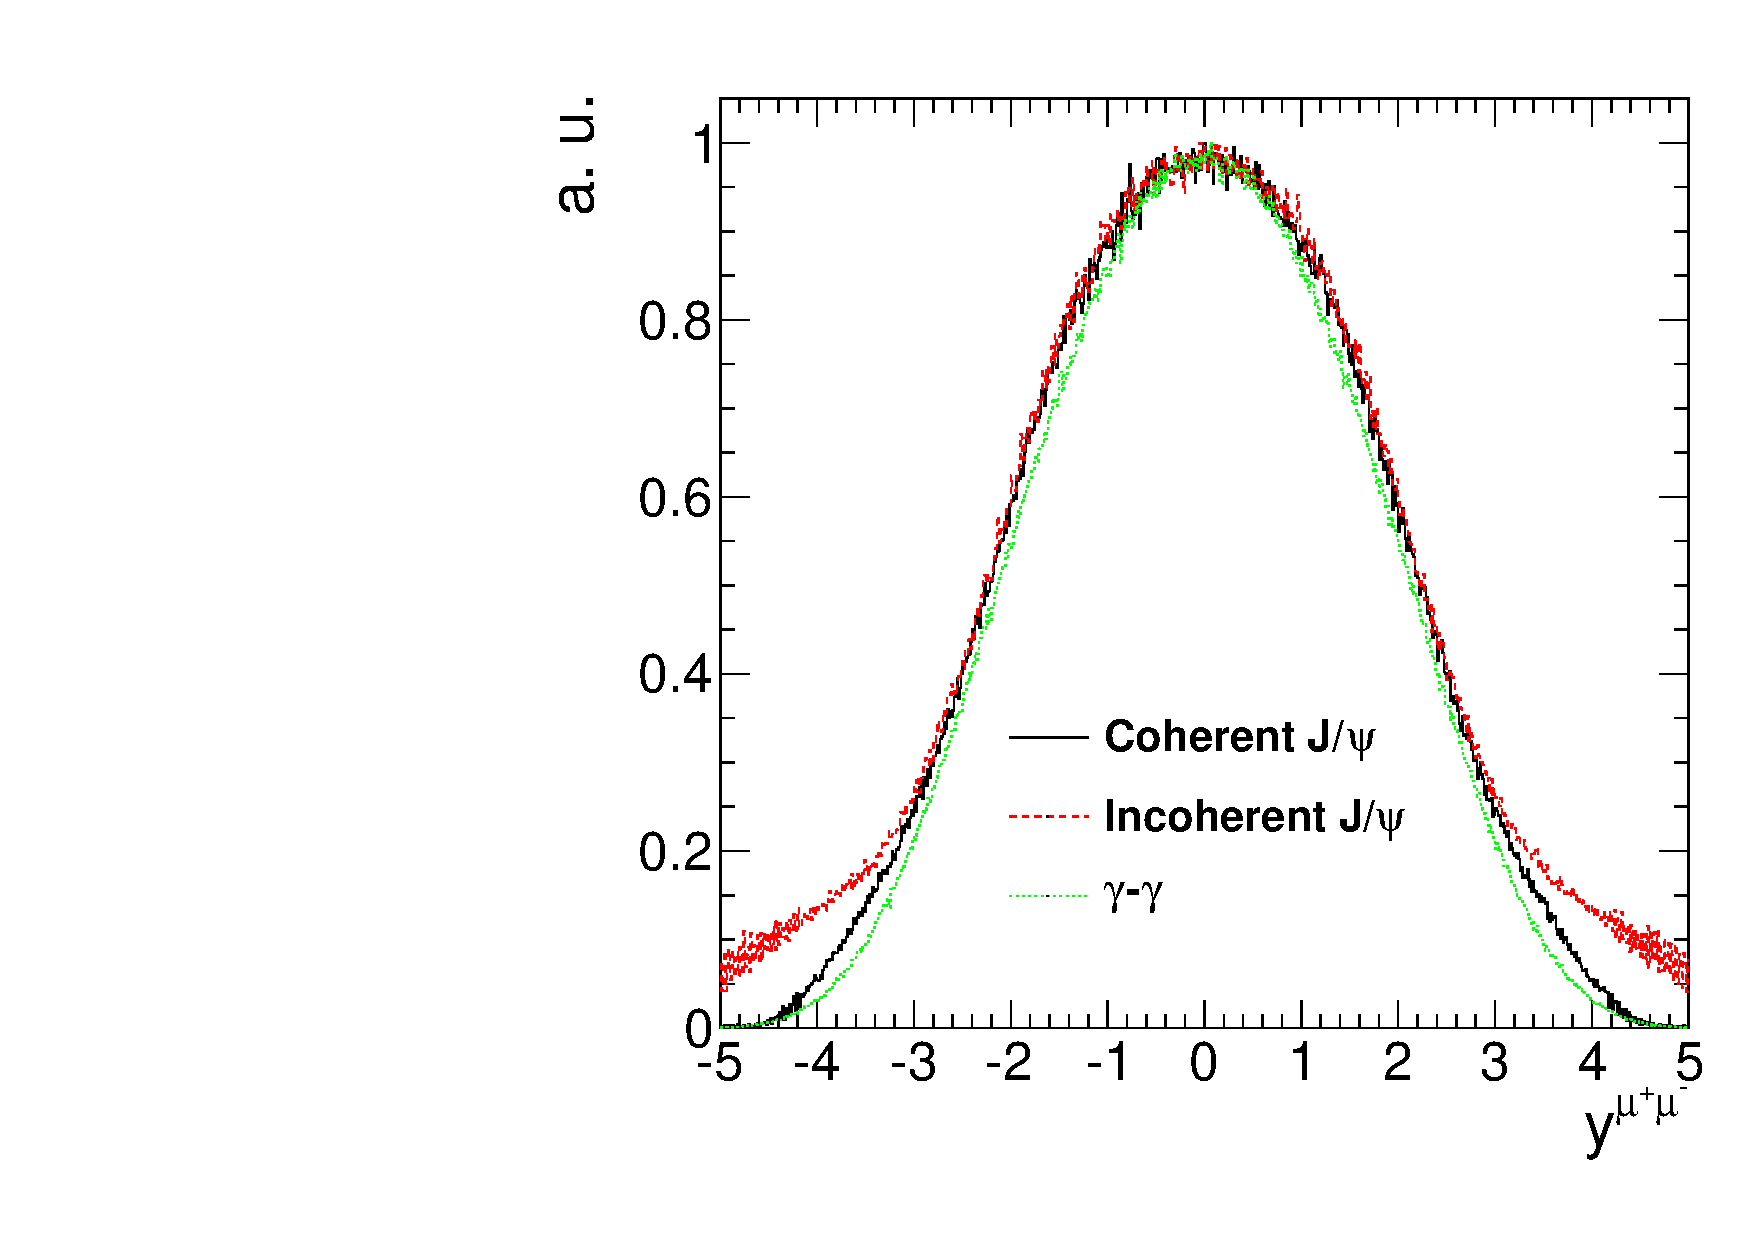
\includegraphics[width=0.45\textwidth]{genRapDis} &
        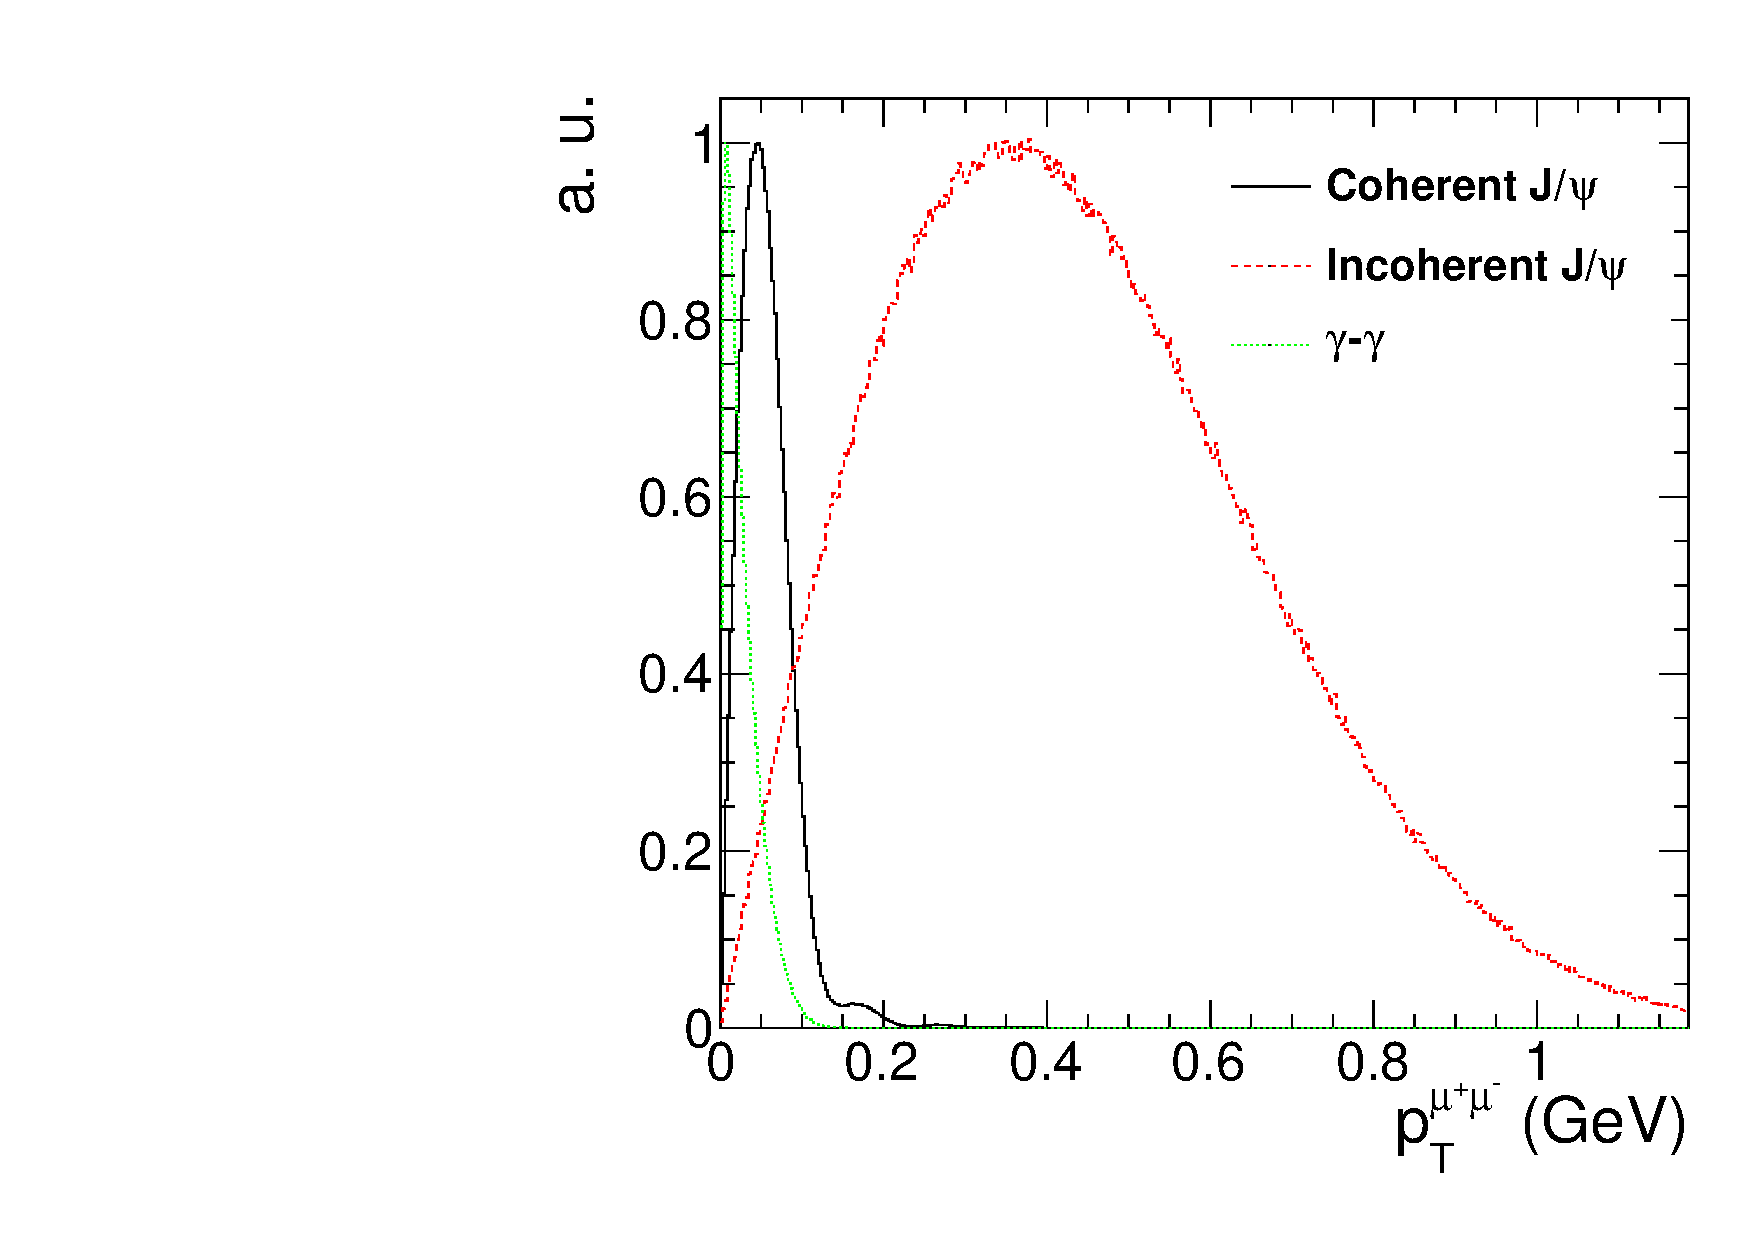
\includegraphics[width=0.45\textwidth]{genPtDis}
      \end{array} $
      \caption{Generator level rapidity (left) and \pt{} (right) 
          distributions for the coherent (black), incoherent (red), 
          and photon-photon process (green).}
      \label{fig:starlightRapPtDist}
    \end{figure}

    The particle gun samples are unpolarized, whereas the STARlight samples 
      have transverse polarization.
    In Fig.~\ref{fig:genHXAngle}, the cosine of the helicity angle of the 
      particle gun samples and the STARlight samples are shown.
    For the STARlight sample the helicity angle, the angle between the 
      direction of the $\mu^{+}$ daughter and the \JPsi{} direction in the rest
      frame of the \JPsi{}, prefer to be either parallel or anit-parallel.
    However, the particle gun samples have no preferred direction of emission.
    \DIFdelbegin %DIFDELCMD < 

%DIFDELCMD <     %%%
\DIFdelend \begin{figure}[!Hhbt]
      \centering
      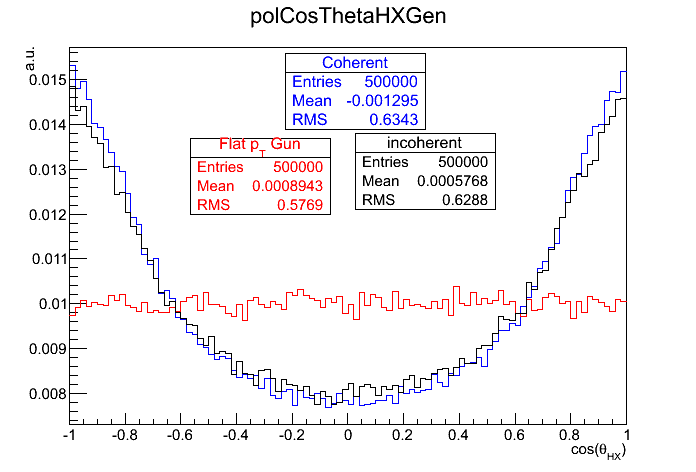
\includegraphics[width=.6\textwidth]{polCosThetaHXGen}
      \caption{ The \JPsi{} polarization of the particle gun (red),
        coherent (blue), and incoherent samples are plotted as the
        cosine of the helicity angle.} 
      \label{fig:genHXAngle}
    \end{figure}

  \DIFdelbegin \section{%DIFDELCMD < \label{sec:TrigDev} %%%
\DIFdel{Trigger development}}
    %DIFAUXCMD
\addtocounter{section}{-1}%DIFAUXCMD
\DIFdel{A collection of triggers was needed in order to select UPC events from the
      collisions at the LHC. 
    The increase in collision rate of the LHC PbPb beams from 2010 to 2011 was
      nearly a factor of 15. 
    To accommodate this increase in rate, the 2011 trigger scheme needed to be 
      more selective than in 2010 where CMS could take any event which 
      appeared to have a collision.
    The available bandwidth was allocated equally amongst the various heavy ion
      analysis groups to pursue as wide a physics program as possible.
    From this consideration, bandwidth limits were placed on the trigger rates
      for each analysis group's trigger package. 
    To ensure that UPC physics could be explored all while respecting the
      goals of the CMS Heavy Ions group as a whole, a UPC triggers were 
      commissioned. 
  }%DIFDELCMD < 

%DIFDELCMD <     %%%
\DIFdel{The UPC trigger rate estimates for commissioning the 2011 triggers were 
      calculated by combining existing triggers from the 2010 run. 
    By calculating the ratio between the UPC trigger rates and the minimum bias
      trigger rate, the UPC trigger rates were scaled up to the anticipated 2011 
      interaction rates using the 2010 data.
    The trigger package for 2011 contained ZDC based efficiency monitoring 
      triggers, muon and electron based triggers for measuring }%DIFDELCMD < \JPsi{}%%%
\DIFdel{, and 
      backup triggers in case there was a problem with the original muon and 
      electron triggers.
}%DIFDELCMD < 

%DIFDELCMD <     %%%
\subsection{%DIFDELCMD < \label{sec:l1Trigger} %%%
\DIFdel{L1 trigger}}
      %DIFAUXCMD
\addtocounter{subsection}{-1}%DIFAUXCMD
\DIFdel{The UPC L1 triggers were designed to record enough data to measure 
        UPC }%DIFDELCMD < \JPsi{} %%%
\DIFdel{production via the dimuon and dielectron channels.
      To achieve this, the loosest muon and electron triggers where paired with
        a trigger on energy in the ZDC were used as a trigger selection 
        criteria, and energy in the BSCs was used as a rejection criteria.
      Additional triggers with rejection criteria based on energy in HF were 
        commissioned in case radiation damage during the run reduced the 
        sensitivity of the BSCs.
      These triggers are summarized in Table~\ref{tab:l1Triggers2011}.
      The 5 and 2 in the ECAL trigger names in Table~\ref{tab:l1Triggers2011}
        indicate a 5 and 2 GeV threshold on $E_{T}$ measured in the ECAL.
      The Open in the muon trigger indicates that the trigger only 
        requires a muon candidate in one of the three muon sub-systems and that
        there is not momentum threshold.
}%DIFDELCMD < 

%DIFDELCMD <       \begin{table}[h]
%DIFDELCMD <         \centering
%DIFDELCMD <         \begin{tabular}{|l|l|l|l|l|}
%DIFDELCMD <           \hline %%%
\DIFdel{L1 trigger }%DIFDELCMD < & %%%
\DIFdel{Rate (Hz) }%DIFDELCMD < & %%%
\DIFdel{Prescale }%DIFDELCMD < & %%%
\DIFdel{Id }%DIFDELCMD < & %%%
\DIFdel{Type }%DIFDELCMD < \\ \hline \hline
%DIFDELCMD <           %%%
\DIFdel{MuonOpen and (ZDC$^{+}$~or~ZDC$^{-}$) and BSC veto }%DIFDELCMD < & %%%
\DIFdel{2.1 }%DIFDELCMD < & %%%
\DIFdel{1 }%DIFDELCMD < & %%%
\DIFdel{1 }%DIFDELCMD < & \multirow{3}{*}{Physics} \\  \hhline{----~}
%DIFDELCMD <           %%%
\DIFdel{ECAL2 and (ZDC$^{+}$~or~ZDC$^{-}$) and BSC veto }%DIFDELCMD < & %%%
\DIFdel{1.8 }%DIFDELCMD < & %%%
\DIFdel{2 }%DIFDELCMD < & %%%
\DIFdel{2 }%DIFDELCMD < & \\  \hhline{----~}
%DIFDELCMD <           %%%
\DIFdel{ECAL5 and (ZDC$^{+}$~or~ZDC$^{-}$) and BSC veto }%DIFDELCMD < & %%%
\DIFdel{0.3 }%DIFDELCMD < & %%%
\DIFdel{1 }%DIFDELCMD < & %%%
\DIFdel{3 }%DIFDELCMD < & \\  \hline
%DIFDELCMD <           %%%
\DIFdel{(ZDC$^{+}$~or~ZDC$^{-}$) }%DIFDELCMD < & %%%
\DIFdel{35 }%DIFDELCMD < & %%%
\DIFdel{1500 }%DIFDELCMD < & %%%
\DIFdel{4 }%DIFDELCMD < & %%%
\DIFdel{Monitor }%DIFDELCMD < \\  \hline
%DIFDELCMD <           %%%
\DIFdel{MuonOpen and (ZDC$^{+}$~or~ZDC$^{-}$) and HF veto }%DIFDELCMD < & %%%
\DIFdel{0 }%DIFDELCMD < & %%%
\DIFdel{off }%DIFDELCMD < & %%%
\DIFdel{5 }%DIFDELCMD < & \multirow{3}{*}{Backup} \\ \hhline{----~}
%DIFDELCMD <           %%%
\DIFdel{ECAL2 and (ZDC$^{+}$~or~ZDC$^{-}$) and HF veto }%DIFDELCMD < & %%%
\DIFdel{0 }%DIFDELCMD < & %%%
\DIFdel{off }%DIFDELCMD < & %%%
\DIFdel{6 }%DIFDELCMD < & \\  \hhline{----~}
%DIFDELCMD <           %%%
\DIFdel{ECAL5 and (ZDC$^{+}$~or~ZDC$^{-}$) and HF veto }%DIFDELCMD < & %%%
\DIFdel{0 }%DIFDELCMD < & %%%
\DIFdel{off }%DIFDELCMD < & %%%
\DIFdel{7 }%DIFDELCMD < & \\  \hline
%DIFDELCMD <         \end{tabular}
%DIFDELCMD <         %%%
%DIFDELCMD < \caption{%
{%DIFAUXCMD
\DIFdel{List of 2011 L1 seeds.}}
        %DIFAUXCMD
%DIFDELCMD < \label{tab:l1Triggers2011}
%DIFDELCMD <       \end{table}
%DIFDELCMD <       %%%
\DIFdel{The cumulative L1 trigger rate for all the UPC L1 trigger seeds was
        required to be no greater than 200 Hz.
      This requirement stemmed from the need to keep the tracker read-out rate
        low. 
      The trackers baseline voltage can fluctuate due to the high tracker hit 
        multiplicities in PbPb collisions.
      In order to monitor the zero suppression of the tracker, the zero 
        suppression algorithm was executed using the HLT computing farm 
	      rather than in the tracker firmware.
}%DIFDELCMD < 

%DIFDELCMD <       %%%
\DIFdel{In order to record the efficiency monitoring data, the ZDC triggers had 
        to be prescaled to a lower rate. 
      The scaling down of the monitoring trigger was setup to ensure overlap
        with the signal triggers.
      The prescales for the triggers were set to balance the competing objectives 
        of rate reduction and increasing the overlap between the monitoring and
        signal triggers.
}%DIFDELCMD < 

%DIFDELCMD <     %%%
\subsection{\DIFdel{HLT trigger}}
      %DIFAUXCMD
\addtocounter{subsection}{-1}%DIFAUXCMD
\DIFdel{An event must pass the selection criteria of an HLT path in order to be
        recorded. 
      As opposed to the L1 trigger, which has access only to information from
        calorimeters and muon chambers, the HLT has access to all of the CMS 
        sub-detectors including the tracker. 
      Reconstruction of a track in the pixel detector is used by the UPC 
        trigger paths.
      The use of the pixel detector only, as opposed to using the whole tracker 
        including the silicon strip detector, allows for quick track 
        reconstruction saving computing cycles.
      The requirement of at least one reconstructed pixel track for the HLT 
        triggers was designed to reject backgrounds where no particles are 
        reconstructed by the tracker.
      For the muon trigger in Table~\ref{tab:hltTriggers2011} the rate was 
        reduced by nearly a factor or 4 compared to its L1 seed rate in 
        Table~\ref{tab:l1Triggers2011}.
      This is due to the additional pixel track requirement. 
      }%DIFDELCMD < \begin{table}[h]
%DIFDELCMD <         \centering
%DIFDELCMD <         \begin{tabular}{|l|l|l|l|l|l|}
%DIFDELCMD <           \hline %%%
\DIFdel{HLT trigger  }%DIFDELCMD < & %%%
\DIFdel{Rate (Hz) }%DIFDELCMD < & %%%
\DIFdel{L1 prescale }%DIFDELCMD < & %%%
\DIFdel{HLT prescale }%DIFDELCMD < & %%%
\DIFdel{L1 seed }%DIFDELCMD < & %%%
\DIFdel{Type }%DIFDELCMD < \\ \hline \hline
%DIFDELCMD <           %%%
\DIFdel{L1UPCMuon and Pixel Track }%DIFDELCMD < & %%%
\DIFdel{0.52 }%DIFDELCMD < & %%%
\DIFdel{1 }%DIFDELCMD < & %%%
\DIFdel{1 }%DIFDELCMD < & %%%
\DIFdel{1 }%DIFDELCMD < & \multirow{3}{*}{Physics} \\ \hhline{-----~} 
%DIFDELCMD <           %%%
\DIFdel{L1UPCECAL2 and Pixel Track }%DIFDELCMD < & %%%
\DIFdel{1.65 }%DIFDELCMD < & %%%
\DIFdel{2 }%DIFDELCMD < & %%%
\DIFdel{1 }%DIFDELCMD < & %%%
\DIFdel{2 }%DIFDELCMD < & \\ \hhline{-----~}
%DIFDELCMD <           %%%
\DIFdel{L1UPCECAL5 and Pixel Track }%DIFDELCMD < & %%%
\DIFdel{0.26 }%DIFDELCMD < & %%%
\DIFdel{1 }%DIFDELCMD < & %%%
\DIFdel{1 }%DIFDELCMD < & %%%
\DIFdel{3 }%DIFDELCMD < & \\ \hline
%DIFDELCMD <           %%%
\DIFdel{L1ZDCOr }%DIFDELCMD < & %%%
\DIFdel{3.6 }%DIFDELCMD < & %%%
\DIFdel{1500 }%DIFDELCMD < & %%%
\DIFdel{11 }%DIFDELCMD < & %%%
\DIFdel{4 }%DIFDELCMD < & \multirow{2}{*}{Monitor}  \\ \hhline{-----~}
%DIFDELCMD <           %%%
\DIFdel{L1ZDCOr and Pixel Track }%DIFDELCMD < & %%%
\DIFdel{2.8 }%DIFDELCMD < & %%%
\DIFdel{1500 }%DIFDELCMD < & %%%
\DIFdel{1 }%DIFDELCMD < & %%%
\DIFdel{4 }%DIFDELCMD < & \\ \hline
%DIFDELCMD <           %%%
\DIFdel{L1UPCMuonHFVeto and Pixel Track }%DIFDELCMD < & %%%
\DIFdel{0 }%DIFDELCMD < & %%%
\DIFdel{off }%DIFDELCMD < & %%%
\DIFdel{off }%DIFDELCMD < & %%%
\DIFdel{5 }%DIFDELCMD < & \multirow{3}{*}{Backup}   \\ \hhline{-----~}
%DIFDELCMD <           %%%
\DIFdel{L1UPCECAL2HFVeto and Pixel Track }%DIFDELCMD < & %%%
\DIFdel{0 }%DIFDELCMD < & %%%
\DIFdel{off }%DIFDELCMD < & %%%
\DIFdel{off }%DIFDELCMD < & %%%
\DIFdel{6 }%DIFDELCMD < & \\ \hhline{-----~}
%DIFDELCMD <           %%%
\DIFdel{L1UPCECAL5HFVeto and Pixel Track }%DIFDELCMD < & %%%
\DIFdel{0 }%DIFDELCMD < & %%%
\DIFdel{off }%DIFDELCMD < & %%%
\DIFdel{off }%DIFDELCMD < & %%%
\DIFdel{7 }%DIFDELCMD < & \\ \hline 
%DIFDELCMD <         \end{tabular}
%DIFDELCMD <         %%%
%DIFDELCMD < \caption{%
{%DIFAUXCMD
\DIFdel{List of 2011 HLT trigger.}}
        %DIFAUXCMD
%DIFDELCMD < \label{tab:hltTriggers2011}
%DIFDELCMD <       \end{table}
%DIFDELCMD < 

%DIFDELCMD <       %%%
\DIFdel{The total HLT output for the UPC trigger package was limited to 20 Hz. 
      The limiting factor for the HLT rate was the amount of disk space 
        available to store the data. 
      To meet the bandwidth requirements and collect a significant sample
        of data for estimating efficiencies, the prescales were balanced with 
        the goal of achieving at least 5\% statistical precision on the 
        efficiency estimates. 
      As an example of the balancing of the prescales, the  ZDC trigger that 
        was passed through from the L1 was given a additional prescale factor 
        of 11 on the HLT.
      The ZDC path that also required a pixel track on the HLT, which used 
        the same L1 seed, was only prescaled at the L1.
      The prescale of 11 was set to ensure that at least 1000 of the pixel track 
        ZDC triggers overlapped with the ZDC L1 only triggers so that efficiency
        of the pixel track requirement in the trigger could be estimated from 
        the tracks lost. 
}%DIFDELCMD < 

%DIFDELCMD <   %%%
\DIFdelend \section{\label{sec:DataSetEvSel} Event selection}
    The unprecedented amounts of data produced by the LHC has made it possible 
      to investigate novel physics processes like UPC \JPsi{} production.
    The data for this analysis were recorded during the 2011 LHC PbPb run. 
    During this period, 150 \DIFdelbegin \DIFdel{$\mu\begin{displaymath}b^{-1}$ \end{displaymath}\DIFdelend \DIFaddbegin \DIFadd{$\mu}b^{-1}$ }\DIFaddend were recorded by the CMS detector,
      corresponding to over a billion PbPb collisions. 
    Of this, 143 \DIFdelbegin \DIFdel{$\mu}b^{-1}$ }\DIFdelend \DIFaddbegin \DIFadd{$\mu$$b^{-1}$ $$\DIFaddend of data were used in this analysis \DIFaddbegin \DIFadd{due to the 
      ZDCs being temporally disconnected to test the Forward Shower Counters}\DIFaddend .

    \subsection{Data sets}
      The data were dived into three specially selected samples, Physics, Monitoring, 
        and Zero bias, based on the triggers which recored the events (see 
        Table~\ref{tab:sampleLumiNevt}).
      By recording this hierarchy of samples, interesting events are selected 
        with a much higher purity in the physics sample, while the zero bias 
        and ZDC triggered samples allow for the investigation of the selection 
        criteria. 
      The purity, which is a measure of how many signal events relative to
        background events are in an sample, is obtained by using more selective
        triggers.
      Less selective triggers, those assigned to the monitoring and zero bias 
        samples, were used to investigate to what extent signal events are lost
        due to the higher selectivity of physics triggers. 
      These samples were recorded using subsets of the HLT triggers found in 
        Table~\ref{tab:hltTriggers2011} of \DIFdelbegin \DIFdel{Section~\ref{sec:TrigDev}}\DIFdelend \DIFaddbegin \DIFadd{Chapter~\ref{ch:trigg}}\DIFaddend .
      The \JPsi{} events discussed in this thesis were obtained analyzing the 
        sample labeled in Table~\ref{tab:sampleLumiNevt} as physics.
      A ZDC triggered monitoring sample was recorded for the sake of estimating
        efficiencies.
      Lastly, a zero bias sample was recored for investigating the ZDC and the 
        noise distributions of HF.

      The physics sample containing the \JPsi{} signal was recorded by the muon 
        trigger labeled "L1UPCMuon and Pixel Track" in 
        Table~\ref{tab:hltTriggers2011}. 
      Because of the characteristically low momentum of UPC \JPsi{} as compared
        to \JPsi{} created by other physics processes, the loosest muon 
        trigger was used.
      The noise trigger rate for the muon trigger alone was \DIFdelbegin \DIFdel{50Hz}\DIFdelend \DIFaddbegin \DIFadd{50 Hz}\DIFaddend , but in 
        coincidence with the BCS veto and the ZDC trigger the noise rate was
        below \DIFdelbegin \DIFdel{2Hz}\DIFdelend \DIFaddbegin \DIFadd{2 Hz}\DIFaddend . 
      By pairing the muon trigger with the ZDC on the L1, the noise contribution
        was reduced from the noise contribution from either of the two 
        sub-detectors to the noise coincidence between the two sub-detectors. 
      Contributions from hadronic interactions are reduced by the veto on the 
        BSCs.
      This trigger was designed to balance reducing the rate with maximizing 
        the efficiency, allowing for the data to be recorded without 
        producing high rates \DIFdelbegin \DIFdel{resulting }\DIFdelend \DIFaddbegin \DIFadd{that would have resulted }\DIFaddend in dead time for the 
        detector.  

      In order to investigate the muon trigger and the other parts of the event 
        selection, a monitoring sample was recorded by requiring energy 
        consistent with at least one neutron in either of the ZDCs.
      Neutron production is \DIFaddbegin \DIFadd{a }\DIFaddend much more common process than the UPC \JPsi{} 
        production.
      This process has cross sections on the order of 100 b compared
        to 10 mb predicted for \JPsi{} production. 
      For this reason, the rates of this trigger are much higher than the physics
        trigger, and only a small sub set of these events are recorded.
      From this trigger the pixel track portion of the HLT trigger efficiency 
        was estimated as well as the ZDC trigger efficiency, as will be described 
        in Section~\ref{sec:effDet}. 

      In addition to the monitoring and physics sample, a zero bias sample was 
        recorded to examine the ZDC neutron reconstruction and the HF noise 
        distributions. 
      The zero bias trigger fired every time both beams passed through CMS. 
      Only 4 events out of every million triggered were recorded for this sample. 
      This sample allowed for an unbiased measurement of the ZDC neutron 
        threshold energies as discussed in Section~\ref{sec:breakUpDet}. 
      Because the zero bias trigger \DIFdelbegin \DIFdel{does not require any activity in any of the CMS sub detectors}\DIFdelend \DIFaddbegin \DIFadd{only requires the presents of both LHC 
        beams}\DIFaddend , the sample contains very few hadronic collisions. 
      This allowed for a measurement of the electronic noise distribution in
        the HF, which are important to reducing contamination from hadronic
        interactions.

      The integrated luminosity for each of the three samples is calculated
        by recording activity in HF \DIFdelbegin \DIFdel{, the forward hadronic calorimeter in CMS
        }\DIFdelend \cite{cmsLumi}. 
      The cross section for HF activity is measured from a van der Meer scan\DIFdelbegin \DIFdel{, 
        and the cross section was found to be 45 mb for proton-proton running}\DIFdelend . 
      In this way, the amount of integrated luminosity for any running period is
        related to the activity in HF. 
      \begin{table}
  	    \centering
  	    \begin{tabular}{|l|l|l|}
  	      \hline Sample & Events & $\mathcal{L}_{int}$ \\ \hline \hline
          Physics & 346K & 143.3 \DIFdelbeginFL \DIFdelFL{$\mu$$b^{-1}$ }\DIFdelendFL \DIFaddbeginFL \DIFaddFL{$\mu}b^{-1}$ }\DIFaddendFL \\ \hline
          Monitor & 1.1M & 31.6 $mb^{-1}$ \\ \hline
          Zero Bias & 8.8M & 580 $b^{-1}$ \\ \hline 
  	    \end{tabular}
  	    \caption{Integrated luminosities and number of events for the three
  	      samples used in this analysis.}
  	    \label{tab:sampleLumiNevt}
      \end{table}

    \subsection{Event selection cuts}
      The analysis described in this thesis focuses on UPC \JPsi{}s decaying to 
        muons. 
      The trigger used for this analysis recored 346841 events.
      A set of off-line cuts were applied to increase the relative contribution 
        of UPC events to background processes. 
      Two sets of event selection cuts were applied to reject background events. 
      The first set rejects background from the beam.
      The second rejects events where hadronic collisions have occurred.
      Table~\ref{tab:evSelCutNumbers} summarizes all the event selection cuts. 
      \DIFdelbegin %DIFDELCMD < 

%DIFDELCMD <       \begin{table}
%DIFDELCMD <         %%%
\DIFdelend \DIFaddbegin \begin{table}[!Hhbt]
        \DIFaddendFL \centering
        \begin{tabular}{|c|c|c|} \hline 
          Cut type & Cut & Events \\ \hline
          -- & all triggered & 346841 \\ \hline
          \multirow{3}{*}{beam background rejection} & good vertex requirement & 340997 \\ \hhline{~--}
          & beam halo muon rejection & 302777 \\ \hhline{~--}
          & cluster shape compatibility requirement & 233590 \\ \hline
          \multirow{3}{*}{hadronic interaction rejection} & single-sided neutron requirement & 149992 \\ \hhline{~--}
          & two track requirement & 32732 \\ \hhline{~--}
          & HF signal rejection & 5392 \\ \hline
          fake muon rejection & muon quality requirement & 2047 \\ \hline
          \multirow{2}{*}{kinematic cut} & \JPsi{} mass requirement & 696 \\ \hhline{~--}
          & muon detectability cuts & 567 \\ \hline
        \end{tabular}
        \caption{Effects of event selection cuts.}
        \label{tab:evSelCutNumbers}
      \end{table}

      To reject beam induced background the following cuts were applied:
      \begin{itemize}
        \item The reconstructed vertex must be within 2 cm in 
          the transverse direction and 25 cm in the 
          longitudinal direction. This cut ensures that reconstructed particles 
          come from interactions between the two beams rather than event where 
          one of the two beams interact with gas particles near the interaction 
          point. 
  	    \item Beam halo muons were rejected using the timing of the muon hits.
          The beam halo cut rejects events where muons surrounding the beam 
          stream through the detector. 
  	    \item Pixel cluster shape should be compatible with the vertex. 
          This cut requires that energy deposits in the silicon tracker point 
            back to the reconstructed  primary vertex. 
      \end{itemize}
      These beam background cuts do not reject any UPC \JPsi{} candidates. 

      The second set of background rejection cuts were designed to 
        reduce contamination from hadronic interactions. 
      \begin{itemize}
  	    \item No more than 2 reconstructed tracks in the event.
          The track requirement rejects events that produce many charged 
          particles.
  	    \item Maximum reconstructed hit energy in HF was required to be below 
            the threshold for electronic noise. 
          Nearly all hadronic interactions (about 98\%) produce particles in 
            the range $3<|\eta|<5$ covered by the HF detector.
          By requiring that the energy deposits in HF resemble noise, nearly all
            elastic hadronic collisions are expected to be rejected.
  	    \item Energy in the ZDCs consistent with neutrons on only one side 
            of the interaction point.
          In hadronic interactions both nuclei break-up. 
          By requiring that ZDC only reconstruct neutrons on one side of the 
            interaction point, hadronic interactions that produce neutrons on 
            both sides were rejected.
      \end{itemize}
      Each of these cuts were designed to reject topologies produced by 
        hadronic interactions.
      The effect of these cuts can be seen in Table~\ref{tab:evSelCutNumbers} 
        and are denoted hadronic interaction rejection. 

      To establish the HF noise thresholds, the noise distributions were 
        measured in zero bias events. 
      An offline selection of events with no reconstructed tracks was used
        to ensure that no collision had taken place. 
      The HF noise threshold was defined as the cut that keeps 99\% of the 
        zero bias events.
      The noise distribution from this zero bias sample is compared to the 
        physics sample and MC in Fig.~\ref{fig:hfNoiseDist}.

      \begin{figure}[!Hhbt]
        \centering
        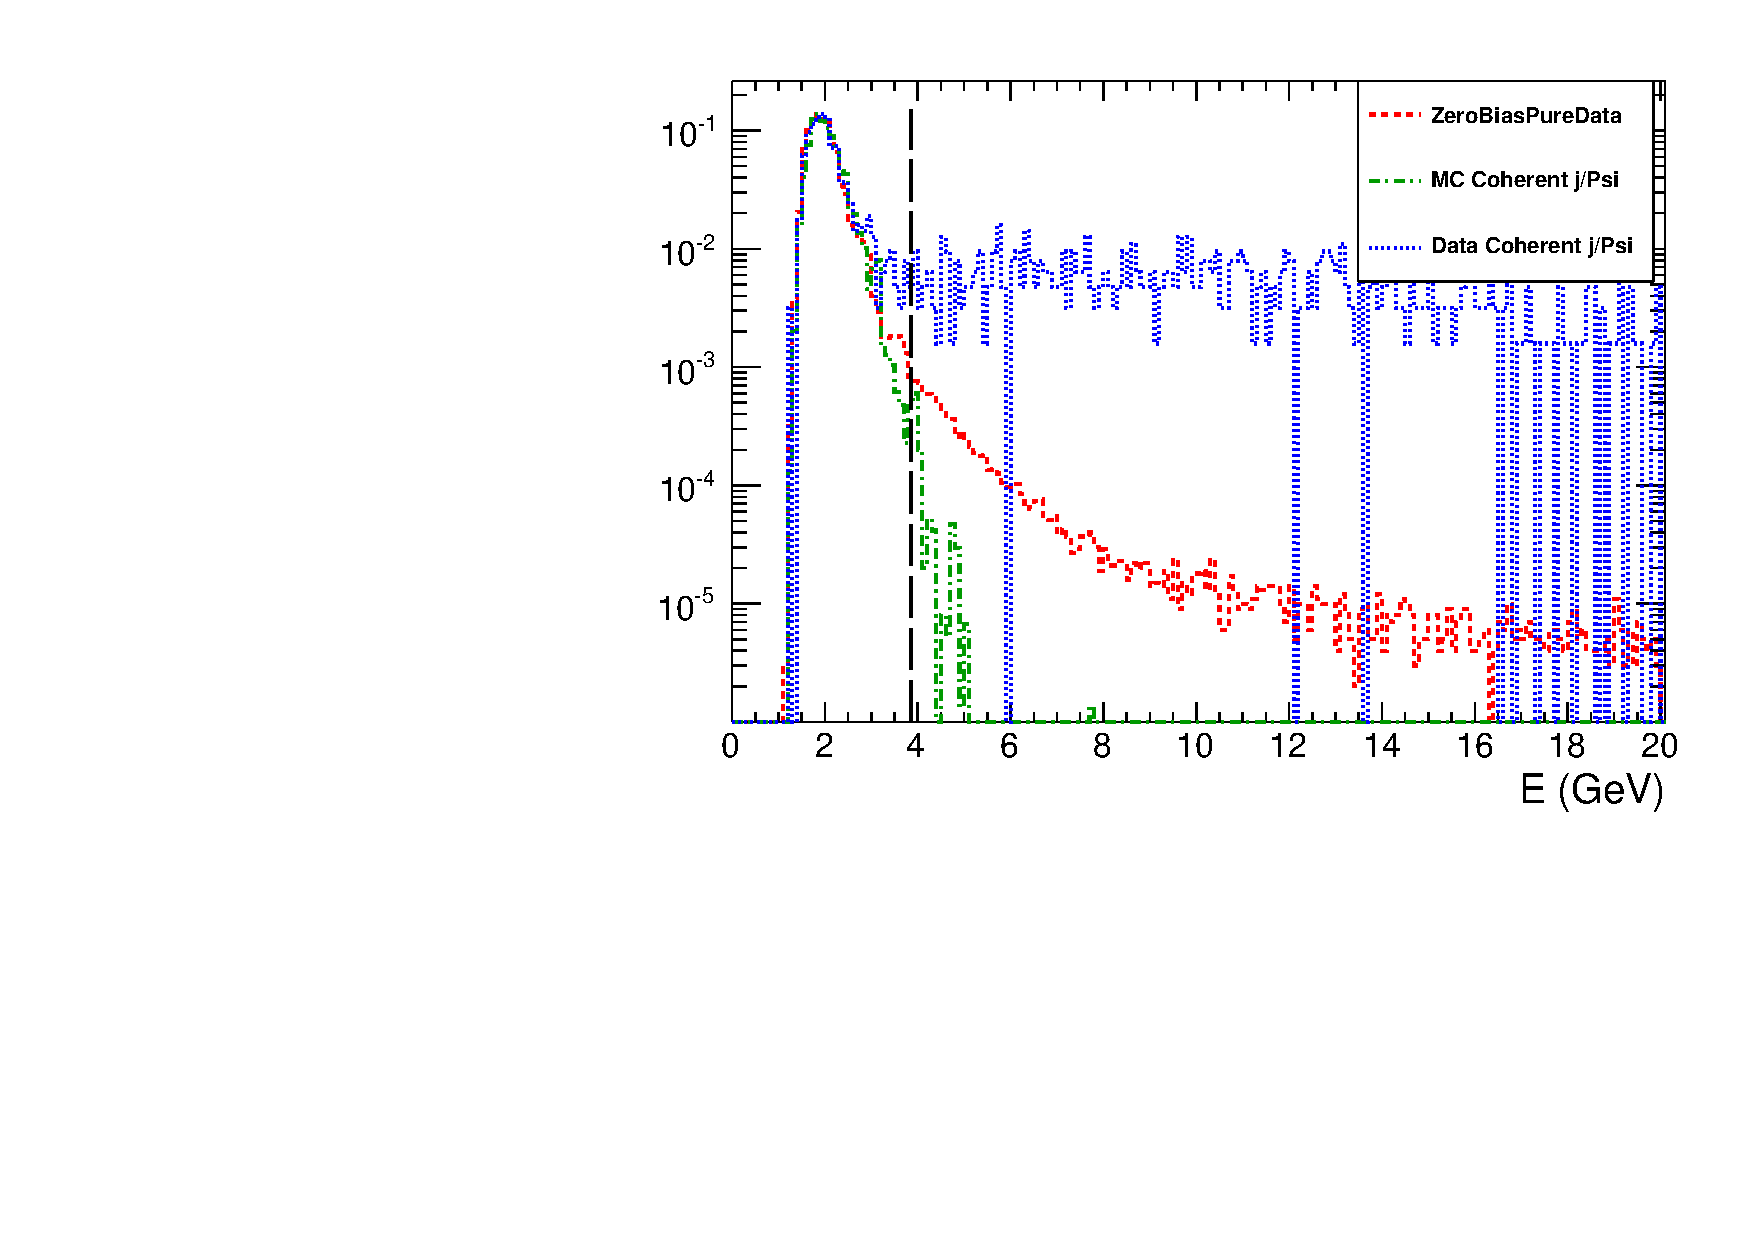
\includegraphics[width=.6\textwidth]{hfNoiseComp}
        \caption{Comparison of HF noise distributions in zero bias data, 
          physics triggered data, and MC.}
        \label{fig:hfNoiseDist}
      \end{figure}

      The following standard muon quality cuts are applied:
      \begin{itemize}
        \item Tracker track matched with at least one muon segment 
          (in any station) in both X and Y coordinates (< 3 $\sigma$).
        \item Cut on number of tracker layers with hits $>$ 5.
        \item Number of pixel layers $>$ 0.
        \item The $\chi^{2}$ per degrees of freedom of the track fit $<$ 3. 
        \item Loose transverse and longitudinal impact parameter cuts, \DIFdelbegin \DIFdel{with in }\DIFdelend \DIFaddbegin \DIFadd{within }\DIFaddend 3 
          cm in the transverse direction and \DIFdelbegin \DIFdel{withing }\DIFdelend \DIFaddbegin \DIFadd{within }\DIFaddend 30 cm in the longitudinal 
          direction with respect to the primary vertex.
      \end{itemize}
      These cuts are applied to reduce the number of fake muons and have been 
        validated for \DIFdelbegin \DIFdel{standard muon analyses }\DIFdelend \DIFaddbegin \DIFadd{other muon analyses \mbox{%DIFAUXCMD
\cite{cmsJpPP}
}%DIFAUXCMD
}\DIFaddend .

  \section{\label{sec:breakUpDet} Break up determination}
    As described in Section~\ref{sec:ltaTheory}, UPC \JPsi{} photoproduction 
      can be accompanied by the emission of neutrons from either of the two 
      colliding nuclei.
    The various neutron emission scenarios, or break-up modes, can 
      be distinguished by the two ZDCs.
    By separating events where the ZDC signal is consistent with 1 neutron 
      versus several neutrons, or where neutrons are present on only one or 
      both sides, the fraction of events which \DIFdelbegin \DIFdel{correspond }\DIFdelend \DIFaddbegin \DIFadd{corresponds }\DIFaddend to a given 
      break-up mode can be measured and compared to theory. 

    In order to maximize the ability to explore the one neutron peak, which 
      sits at the bottom of the ZDCs dynamic range, a new ZDC reconstruction 
      method was devised. 
    This new reconstruction method was then used to establish a one neutron and
      many neutron threshold.
    This section describes the ZDC signal reconstruction and how the neutron 
      thresholds on this signal were set.

    \subsection{ZDC signal reconstruction}
      The signal from each ZDC is built up from the pulse shapes for each of 
        the 18 individual ZDC channels. 
      The pulse shape is recorded in 250 ns second chunks and is divided into
        10 time slices of 25 ns (\DIFdelbegin \DIFdel{See }\DIFdelend \DIFaddbegin \DIFadd{see }\DIFaddend Fig~\ref{fig:zdcPulseShape}).
      Counting from 0, the 4th time slice is synced with the timing of the rest
        of the detector and corresponds to when the products of the recorded 
        collision reached the ZDC.
      The channel signal is therefore taken from the 4th time slice.
      \begin{figure}[h]
        \centering
        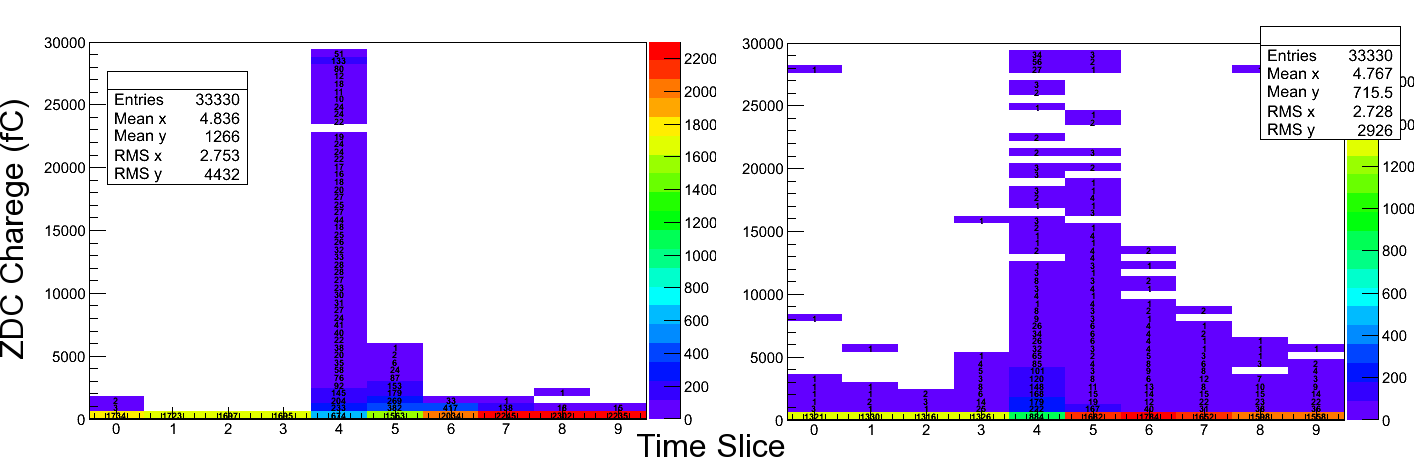
\includegraphics[width=\textwidth]{zdcPulseShape}
        \caption{Average ZDC pluse shape is plotted as the charge as a function
          of time slice for the first hadronic from ZDC$^{-}$ (left) and 
          ZDC$^{+}$ (right).}
        \label{fig:zdcPulseShape}
      \end{figure}

      The ZDC signal sits on top of a low frequency noise pedestal with a 
        period of about 2$\mu$ seconds. 
      Over the time scale of 250 ns, this low frequency noise signal appears
        as a constant that shifts randomly from event to event.
      The contribution from this noise is therefore measured event by event
        in order to subtract it.
      Time slice 5 is used for this purpose.
      Time slices 1 and 2 could also be used to estimate the low frequency 
        noise.
      However because the noise fluctuates to negative values of charge that 
        cannot be measured, these time slices can only provide a 
        measurement of the noise half the time. 
      By using time slice 5 which contains the falling tail of the signal, 
        the noise can be measured any time the signal raises significantly 
        above the noise.
      If the fraction of signal in time slice 4 and 5 are constant and
        the noise contributes the same value to both time slices, the 
        following formula is applicable:
      \begin{equation}
        Ts4 \propto (Ts4 + C) - ( Ts5 + C ) = Ts4 - R_{Ts5/Ts4}Ts4 
        = Ts4(1-R_{Ts5/Ts4}),
        \label{eq:ts4ish}
      \end{equation}
      where $Ts4$ is the signal contribution in time slice 4, $Ts5$ is the 
        signal contribution to time slice 5, $C$ is a random noise constant
        from the low frequency noise, and $R_{Ts5/Ts4}$ is the ratio between
        the signal contribution from time slice 5 over time slice 4.
      Figure~\ref{fig:zdcTs4OvTs5VTs5} demonstrates the \DIFdelbegin \DIFdel{consistence }\DIFdelend \DIFaddbegin \DIFadd{consistency }\DIFaddend of the 
        fraction and validates the unconventional method of using the falling 
        tail of the signal to estimate the low frequency noise. 
      By using time slice 5, the chances of measuring the noise are maximized. 
      Separating the signal from the noise is especially important because
        the ZDC signal for the one neutron peak sits near the noise at the 
        bottom of the ZDC dynamic range.
      \begin{figure}[!Hhbt]
        \centering
        $ \begin{array}{cc}
          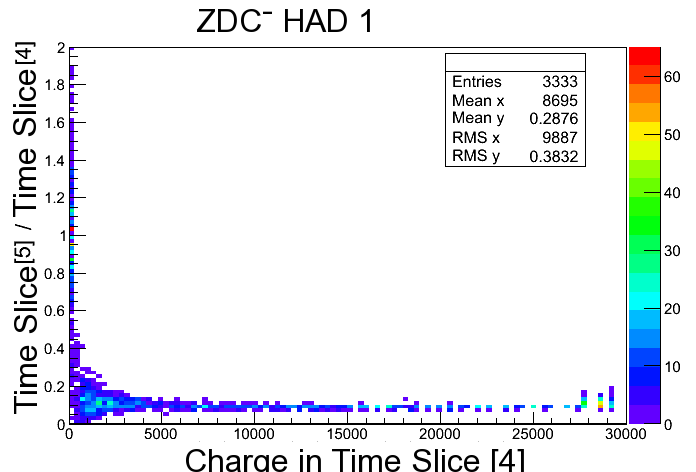
\includegraphics[width=.4\textwidth]{negTs5overTs4vts5} &
          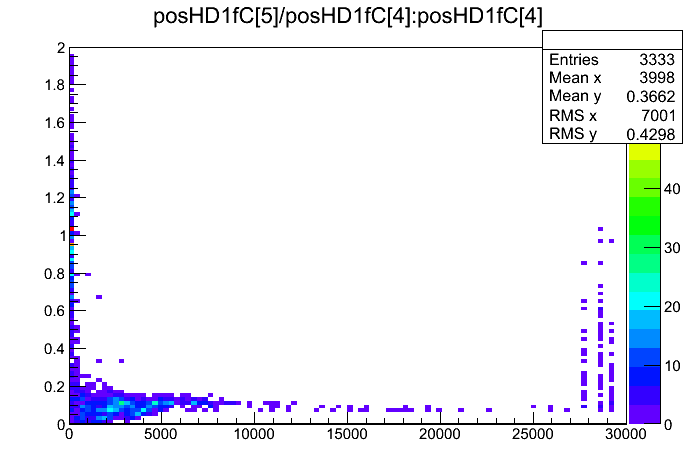
\includegraphics[width=.4\textwidth]{posTs5overTs4vts5}
        \end{array} $  
        \caption{ The fraction of signal in time slice 5 over time slice 4 
          as a function of the signal in time slice 5 in ZDC$^{-}$ (left) and 
          ZDC$^{+}$ (right).}
        \label{fig:zdcTs4OvTs5VTs5}
      \end{figure}

      When summing the 9 channels in each ZDC only channels with signals above 
        zero in time slices 4 and 5 were included. 
      The EM, electromagnetic, section of the calorimeter is more densely 
        packed with quartz fibers and therefore has a higher gain relative to 
        the HAD, hadronic, section. 
      To account for this, the EM channels were weighted with
        a factor of 0.1 to match the HAD channel gains.

    \subsection{Determination of the one neutron thresholds}
      The ZDC thresholds used to establish the various break-up modes were 
        measured from zero bias data.
      Figure~\ref{fig:zdcM2Fit} shows the weighted sum of the EM and 
        HAD sections for  ZDC$^{-}$ and  ZDC$^{+}$ for the zero bias 
        dataset.
      The neutron spectrum for this dataset \DIFdelbegin \DIFdel{does }\DIFdelend is biased since the 
        trigger only required that both beams were present in CMS. 
      This does, however, include a significant electronic noise contribution due
        to events where no neutrons are emitted in the direction of the ZDC.
      It is clear from Fig.~\ref{fig:zdcM2Fit} that the gain of  
        ZDC$^{+}$ is lower than that of ZDC$^{-}$. 
      This is because of a damaged phototube on the first HAD section 
        of ZDC$^{+}$.

      To determine the thresholds for one and multiple neutrons, the ZDC$^{+}$ 
        and ZDC$^{-}$ spectra were fit.
      Four Gaussian functions were combined to fit the spectra. 
      The electronic noise was fit to a Gaussian around zero.
      The one, two, and three neutron peaks are fit to Gaussians that are 
        successively broader.
      The mean of each peak was initially set to multiples of the mean of the 
        one neutron peak. 
      \begin{figure}[!Hh]
        \centering
        $ 
          \begin{array}{cc}
            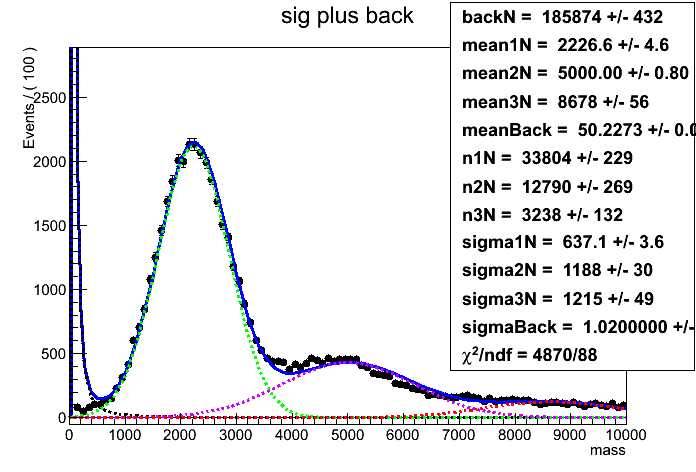
\includegraphics[width=0.45\textwidth]{zdcFit45Neg} &
            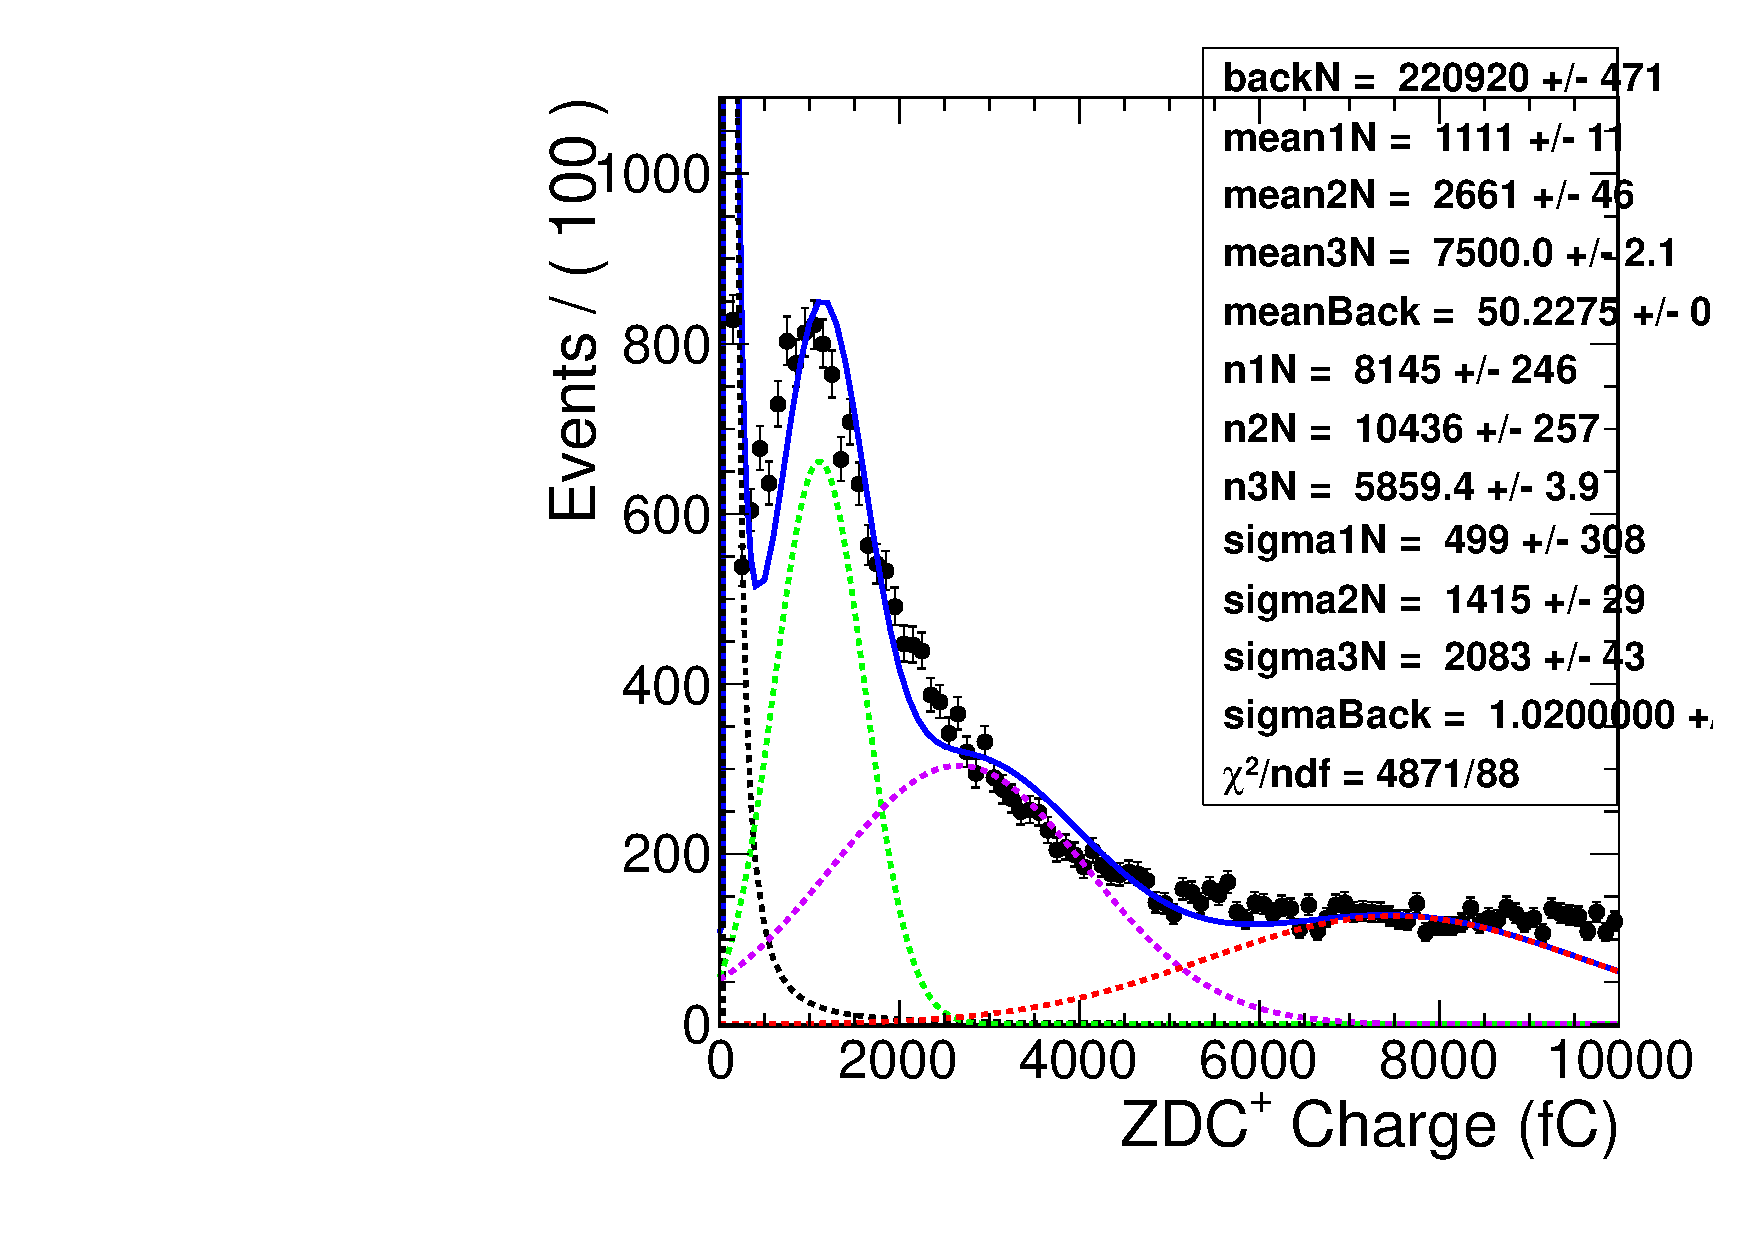
\includegraphics[width=0.45\textwidth]{zdcFit45Pos}
          \end{array} 
        $
        \caption{Fit to the signal spectra for ZDC$^{-}$ (left) and ZDC$^{+}$ 
          (right)}
        \label{fig:zdcM2Fit}
      \end{figure}
      The threshold for a neutron in the ZDC was taken from the fits in 
        Fig.~\ref{fig:zdcM2Fit}.
      Any signal greater 2$\sigma$ below the mean of the one neutron peak was 
        considered signal.
      Any signal greater than 2$\sigma$ above was considered multiple 
        neutrons.
      The single neutron break up modes were separated from the multiple 
        neutron modes by use of these definitions.

      Several of the break-up mode calculations that have been done involve
        single sided configurations where neutrons are present on one side
        of the interaction point and not the other.
      These modes can be hard to identify because the single neutron peak in 
        ZDC$^{+}$ overlaps with the noise peak at zero.
      To identify events where the ZDCs only measured noise, the noise
        spectrum were measured directly.
      Placing an additional criteria based on the ZDCs noise distributions for
        when the ZDCs are devoid of signal provides assurance that the events 
        tagged as single sided events are truly single sided.

      
      The noise distributions for the EM sections and the HAD sections were
        measured separately from out of time time slices.
      In Fig.~\ref{fig:zdcPulseShape} higher than average signal can be seen
        in the 0th time slice, which precedes the main signal time slice 
        time slice 4 by 200 ns. 
      This is due to events where activity was present in the ZDC for 
        two consecutive collisions.
      Time slices 1 and 2, however, occurred between collisions.
      These time slices, which occur out of time, were used to measure the 
        noise spectrum.
      \begin{figure}[!Hhbt]
        \centering
        $ \begin{array}{cc}
          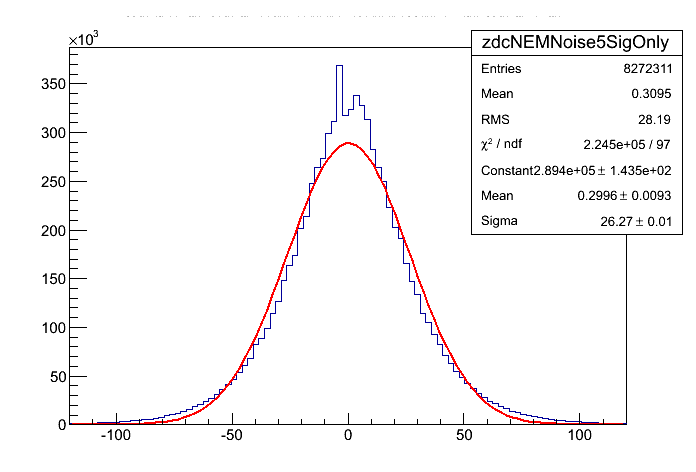
\includegraphics[width=.45\textwidth]{zdcNegEMNoiseFromZBNoCor} & 
          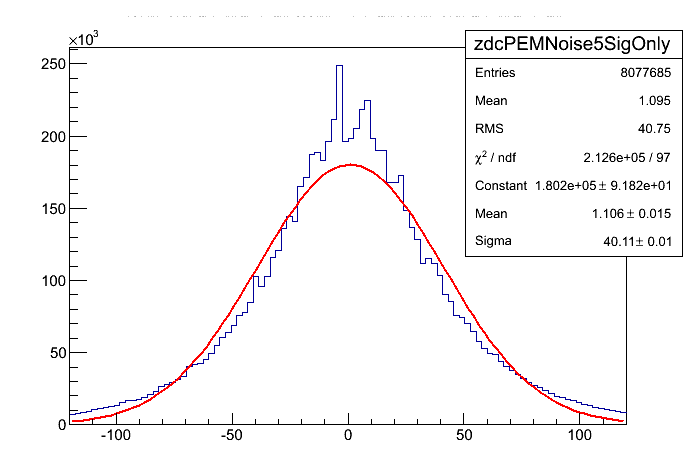
\includegraphics[width=.45\textwidth]{zdcPosEMNoiseFromZBNoCor} \\
          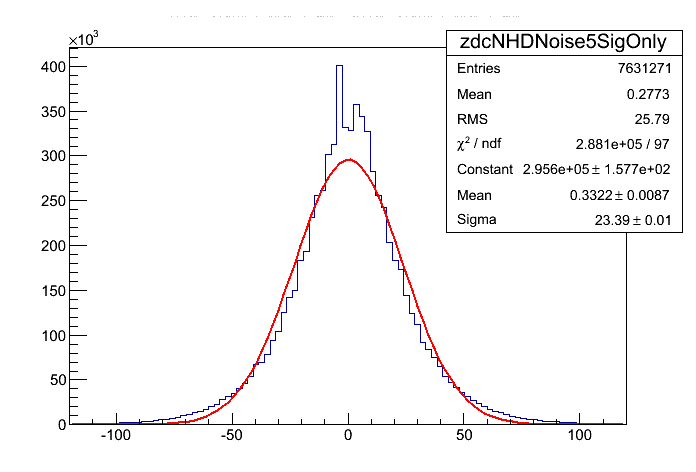
\includegraphics[width=.45\textwidth]{zdcNegHDNoiseFromZB} &
          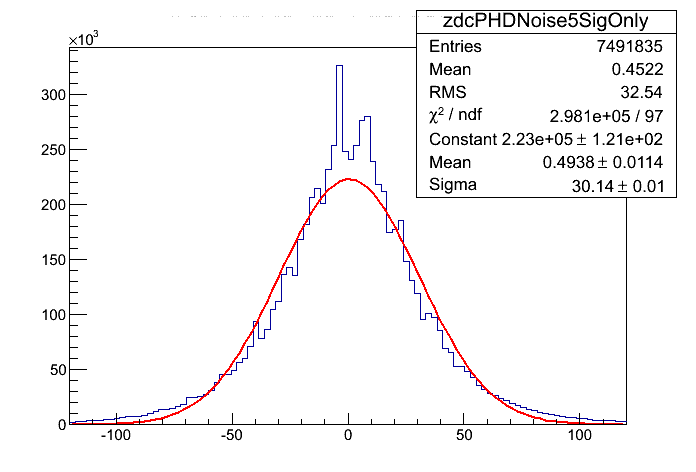
\includegraphics[width=.45\textwidth]{zdcPosHDNoiseFromZB}
        \end{array} $
        \caption{ZDC noise spectra from ZDC$^{-}$ EM section (upper left), 
          ZDC$^{+}$ EM section (upper right), ZDC$^{-}$ HAD section (lower left), 
          and ZDC$^{+}$ HAD section (lower right) from out of time time slices.}
        \label{fig:zdcNoiseSpectra}
      \end{figure}

      As with the signal measurements, the low frequency noise pedestal is 
        subtracted event by event by subtracting time slice 2 from time slice
        1 leaving only the high frequency noise.
      The noise distributions do not depend on the amount of quartz fibers, but
        because the signal does, the noise distributions for EM and HAD sections
        are measured separately.
      \DIFdelbegin \DIFdel{Fig}\DIFdelend \DIFaddbegin \DIFadd{Figure}\DIFaddend ~\ref{fig:zdcNoiseSpectra} shows the noise spectrum for each of the 
        EM and HAD sections for the two ZDCs.
      If the HAD or EM signals measured from time slices which match the 
        timing for a collision, time slices 4 and 5, are less than 2$\sigma$ 
        above the mean of the noise distribution or lower, these sections are 
        considered consistent with noise.
      A ZDC is considered consistent with noise if both the HAD section and EM 
        section from that ZDC have signal measurements consistent with noise.

  \section{\label{sec:sigEx} Signal extraction}
    After all event selection cuts, the remaining events contain a combination 
      of coherent \JPsi{}, incoherent \JPsi{}, and dimuons from the 
      photon-photon process.
    Each process must be separated from the final mix.
    To achieve this, the invariant mass and \pt{} distributions are used 
      to distinguish between the three processes. 
    The photon-photon process is extended in invariant mass whereas the 
      \JPsi{} is peak strongly near 3.1 GeV.
    In dimuon transverse momentum distribution of the photon-photon and 
      coherent process have similar distributions, both peaked shapely below 
        0.1 GeV, whereas the incoherent process is more broadly distributed 
        across an interval extending to nearly 1 GeV.
    The mass distribution was fit to separate the photon-photon process from
      the \JPsi{} process.
    The \pt{} distribution was used to separate the incoherent process from 
      the photon-photon process, and the coherent process. 
    In this way, a separate yield was extracted for all three processes. 

    The invariant mass distribution for opposite sign dimuons is shown in 
      Fig.~\ref{fig:massFit}. 
    A \JPsi{} signal is clearly visible together with tails at higher and
      lower mass due to the photon-photon process.
    A fit to the invariant mass distribution was \DIFdelbegin \DIFdel{done }\DIFdelend \DIFaddbegin \DIFadd{performed }\DIFaddend using a Gaussian
      to account for the \JPsi{} signal and a \DIFdelbegin \DIFdel{first order }\DIFdelend \DIFaddbegin \DIFadd{first-order }\DIFaddend polynomial function 
      for the photon-photon process.
    The extracted number of \JPsi{} candidates from this fit includes all 
      \JPsi{}s in the mass window that passed the analysis cuts, i.e. both
      coherent and incoherent process contribute to yield from the mass
      fit.
    The \pt{} distribution is needed to separate the two different 
      contributions to the \JPsi{} peak. 

    \begin{figure}[!Hhtb]
      \centering
      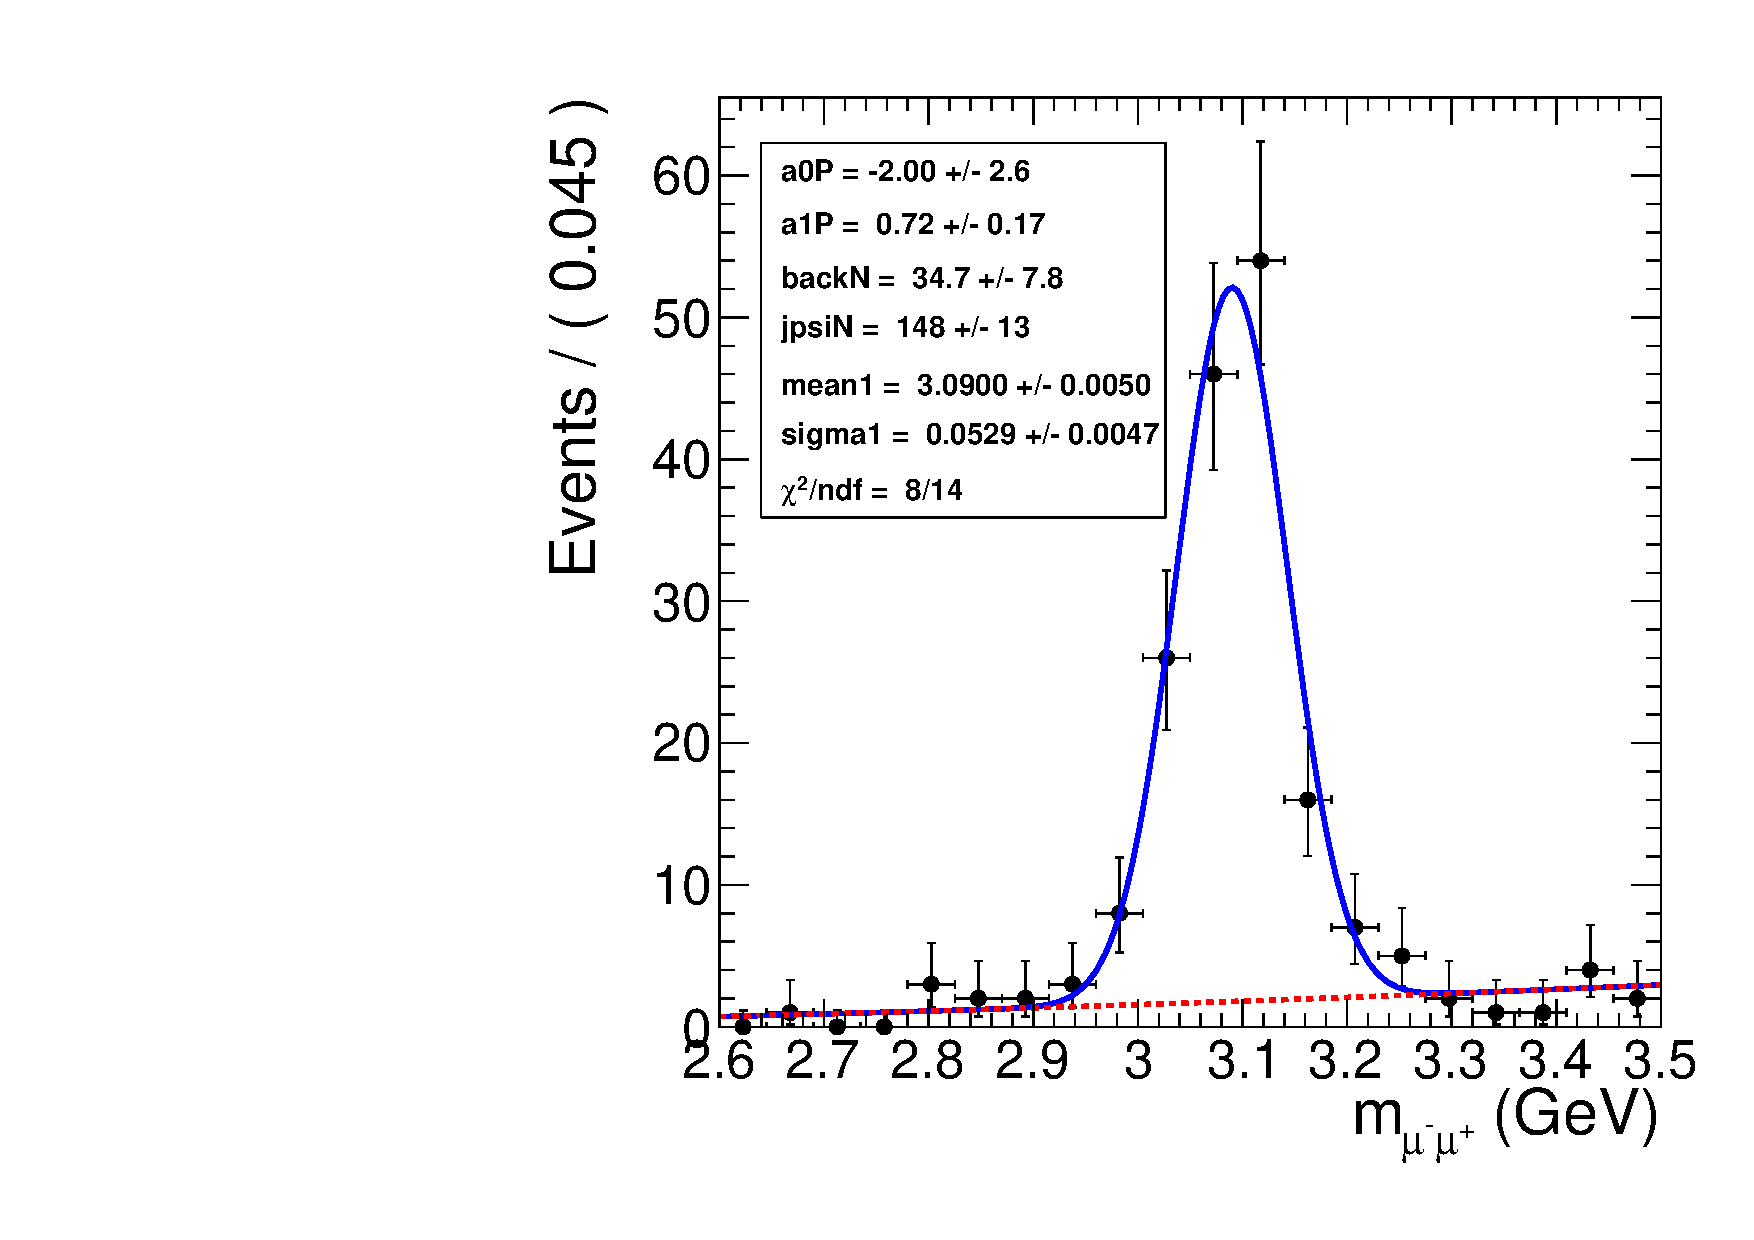
\includegraphics[width=.6\textwidth]{massFitSimple}
      \caption{Mass fit to \JPsi{} using Gaussian for the 
        signal and a \DIFdelbeginFL \DIFdelFL{first order }\DIFdelendFL \DIFaddbeginFL \DIFaddFL{first-order }\DIFaddendFL polynomial for the photon-photon continuum\DIFaddbeginFL \DIFaddFL{.}\DIFaddendFL }
      \label{fig:massFit}
    \end{figure}

    Figure~\ref{fig:ptTemps} shows the \pt{} spectrum of the events plotted 
      in Fig.~\ref{fig:massFit}.  
    There is a clear coherent peak at \pt{} = 60 MeV followed by broad 
      distribution that peaks near \pt{} = 450 MeV. 
    To extract the contribution of coherent, incoherent and gamma-gamma 
      processes in the data the spectrum in  Fig.~\ref{fig:ptTemps} was fit to 
      the sum of three MC templates corresponding to the final output of the MC
      simulations for these three processes.       
    The clear overlap of the coherent and photon-photon process, and the 
      clear separation of these two lower \pt{} processes from the incoherent
      process is apparent.
    The shape of the \pt{} distribution for the coherent, incoherent, and 
      photon-photon process are taken from the final output of MC after
      applying all analysis cuts. 
    In Fig.\ref{fig:ptTemps}, the yield parameters that were fit were left
      unconstrained for all three process.

    \begin{figure}[!Hhbt]
      \centering
      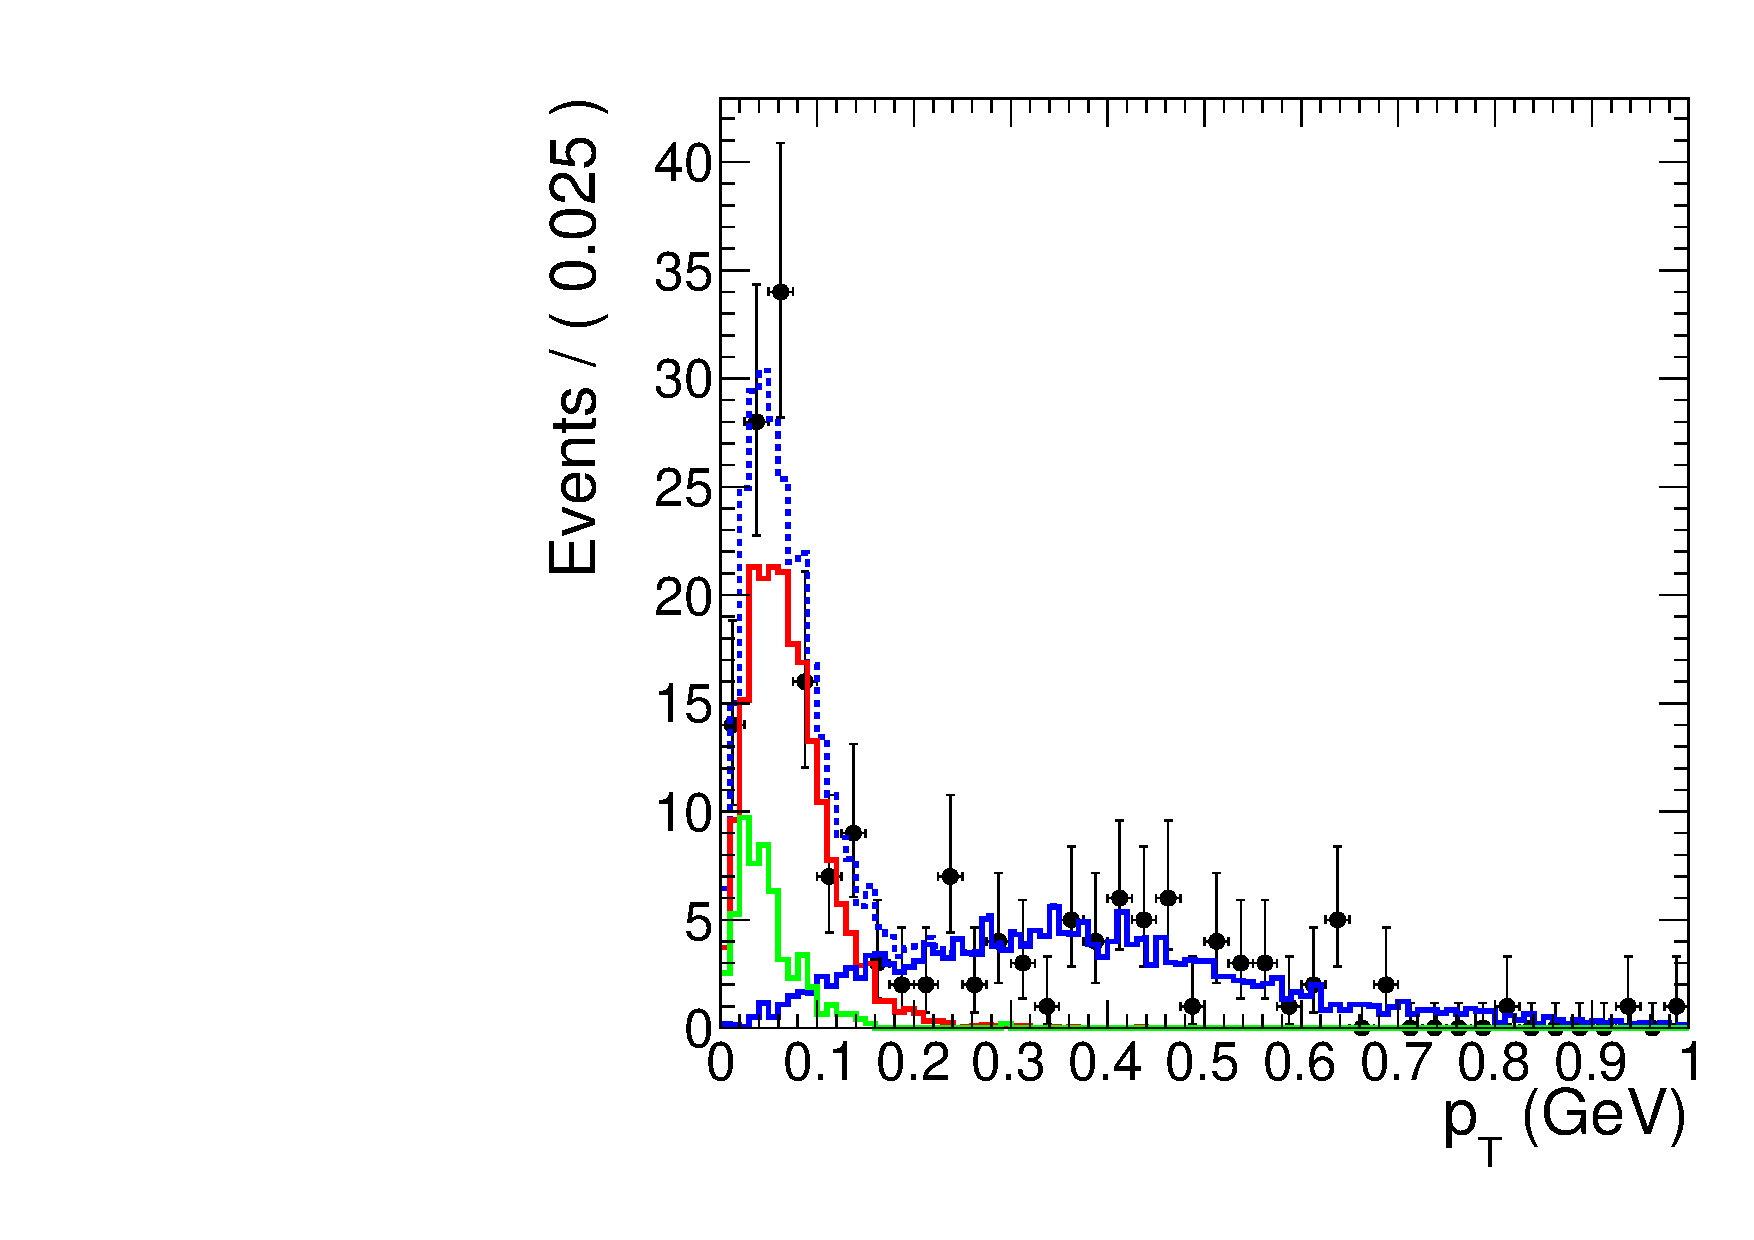
\includegraphics[width=.6\textwidth]{ptOnly}
      \caption{ Fit to MC \pt{} templates. }
      \label{fig:ptTemps}
    \end{figure}

    The shape of the photon-photon and coherent \JPsi{} process are very 
      similar in transverse momentum.
    Accordingly, the contribution from the photon-photon process and the 
      coherent process are difficult to separate from the \pt{} distribution.
    The confidence contours in Fig.~\ref{fig:ptOnlyCor} from the template fit
      in Fig.~\ref{fig:ptTemps} demonstrate the strong anti-correlation 
      between the coherent yield parameter, $nCo$, and the yield parameter 
      for the photon-photon process, $nGamma$.
    Because of the anti-correlation, the statistical uncertainty on $nCo$ and 
      $nGamma$ from the fit are larger than $\sqrt{nCo}$ and $\sqrt{nGamma}$
      expected from Poisson statistics. 
    The information from the invariant mass and \pt{} distributions were
      combined to break this correlation. 
    Through this combination, the contribution to the final yield from 
      the three process was measured.

    \begin{figure}[!Hhbt]
      \centering
      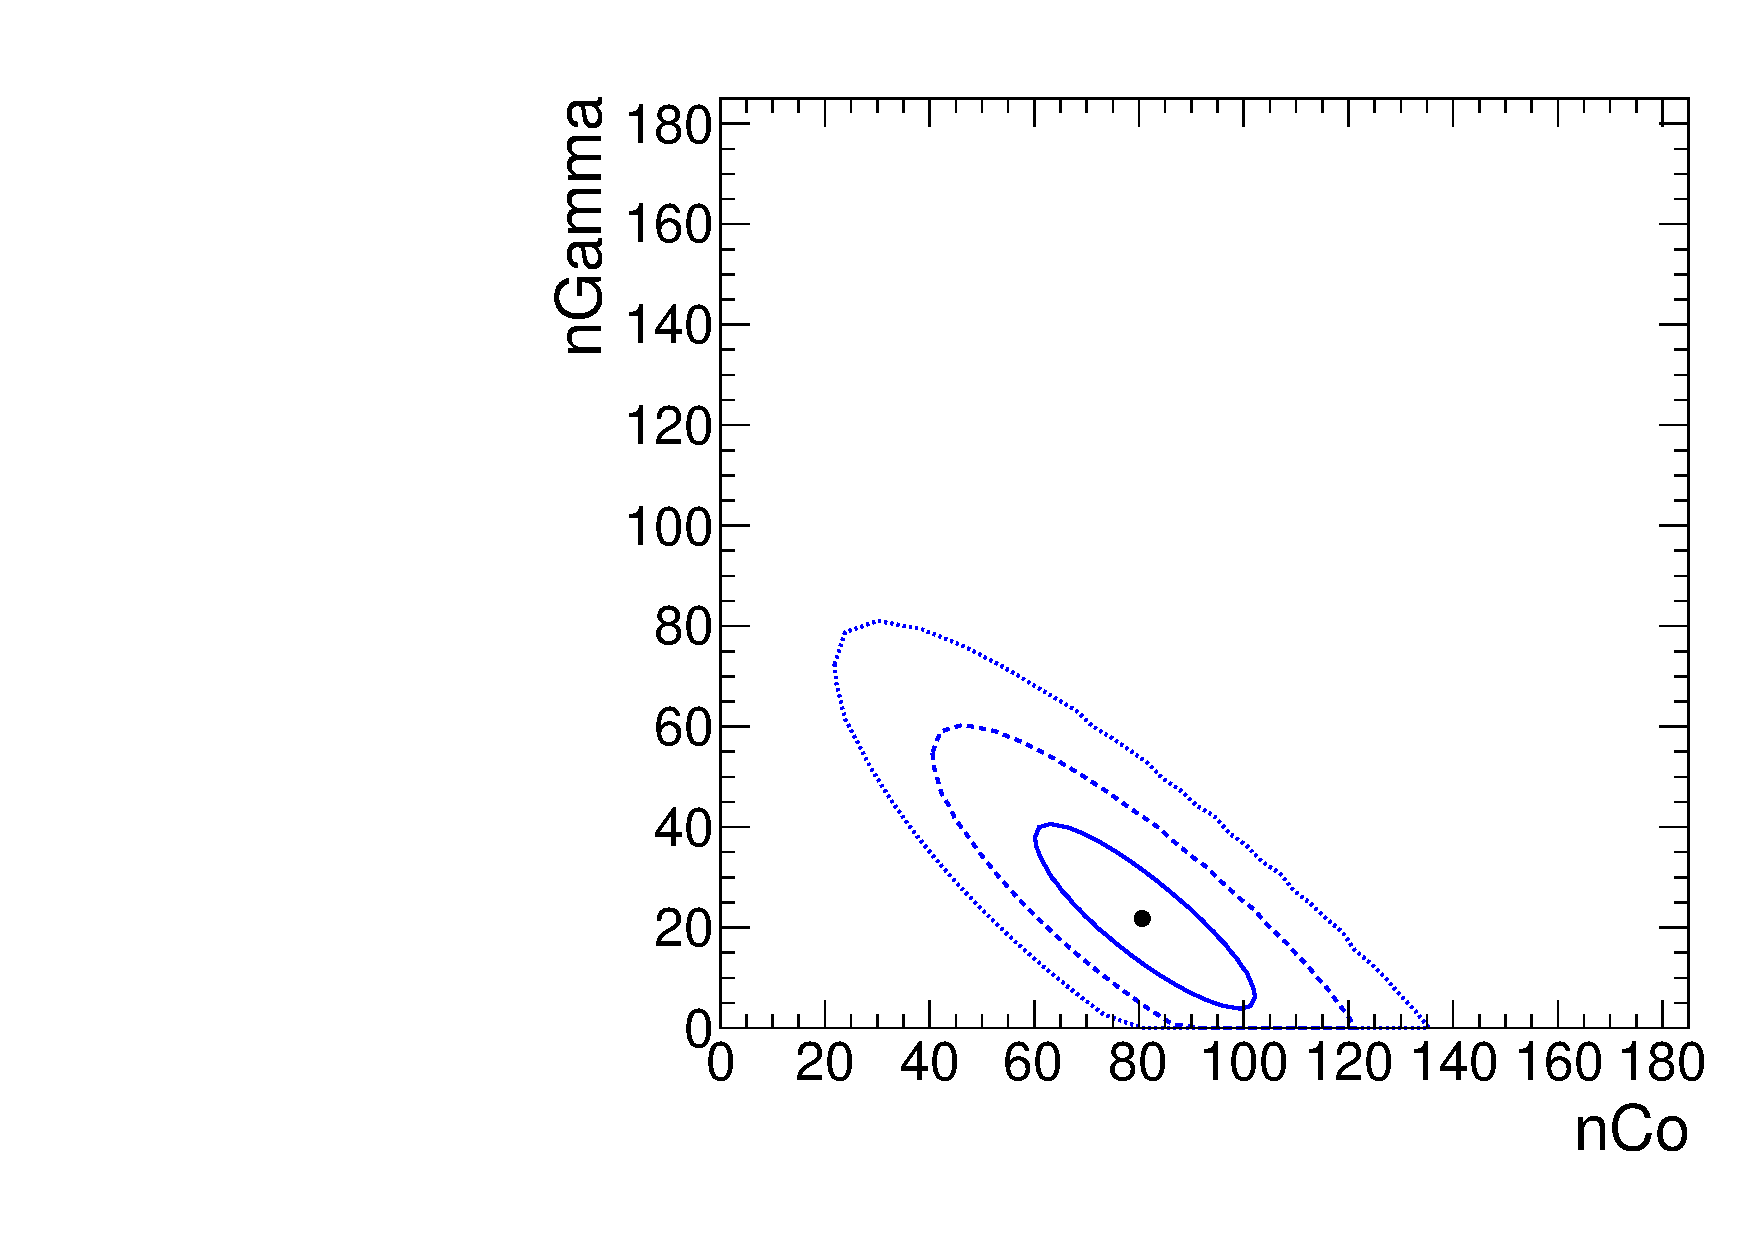
\includegraphics[width=.6\textwidth]{nCoNGammaCorPtOnly}
      \caption{68\%, 95\%, and 99\% confidence contours from the \pt{} 
        template fit. }
      \label{fig:ptOnlyCor}
    \end{figure}

    A simultaneous fit to the mass spectrum and \pt{} 
      spectrum was preformed to utilize the mass fits ability to distinguish 
      the photon-photon process from the coherent and incoherent process all 
      while utilizing the \pt{} fits ability to separate the coherent and 
      photon-photon processes from the incoherent.
    Fig.~\ref{fig:simFitMassPtGauss} shows the result of the simultaneous fit.
    The simultaneous fit forces the parameter $nGamma$ to both describe the 
      photon-photon continuum present in the side bands of the \JPsi{} mass 
      peak as well the photon-photon contribution to the low-\pt{} part of 
      the \pt{} spectrum.
    In addition, the \JPsi{} yield from the mass fit is forced to equal the
      contribution from the incoherent and coherent process in the 
      fit to the \pt{} distribution. 
    In this way, the correlation between the yield parameters was broken, and 
      the contribution from the three process were made independent of each 
      other.

    \begin{figure}[!Hhbt]
      \centering
      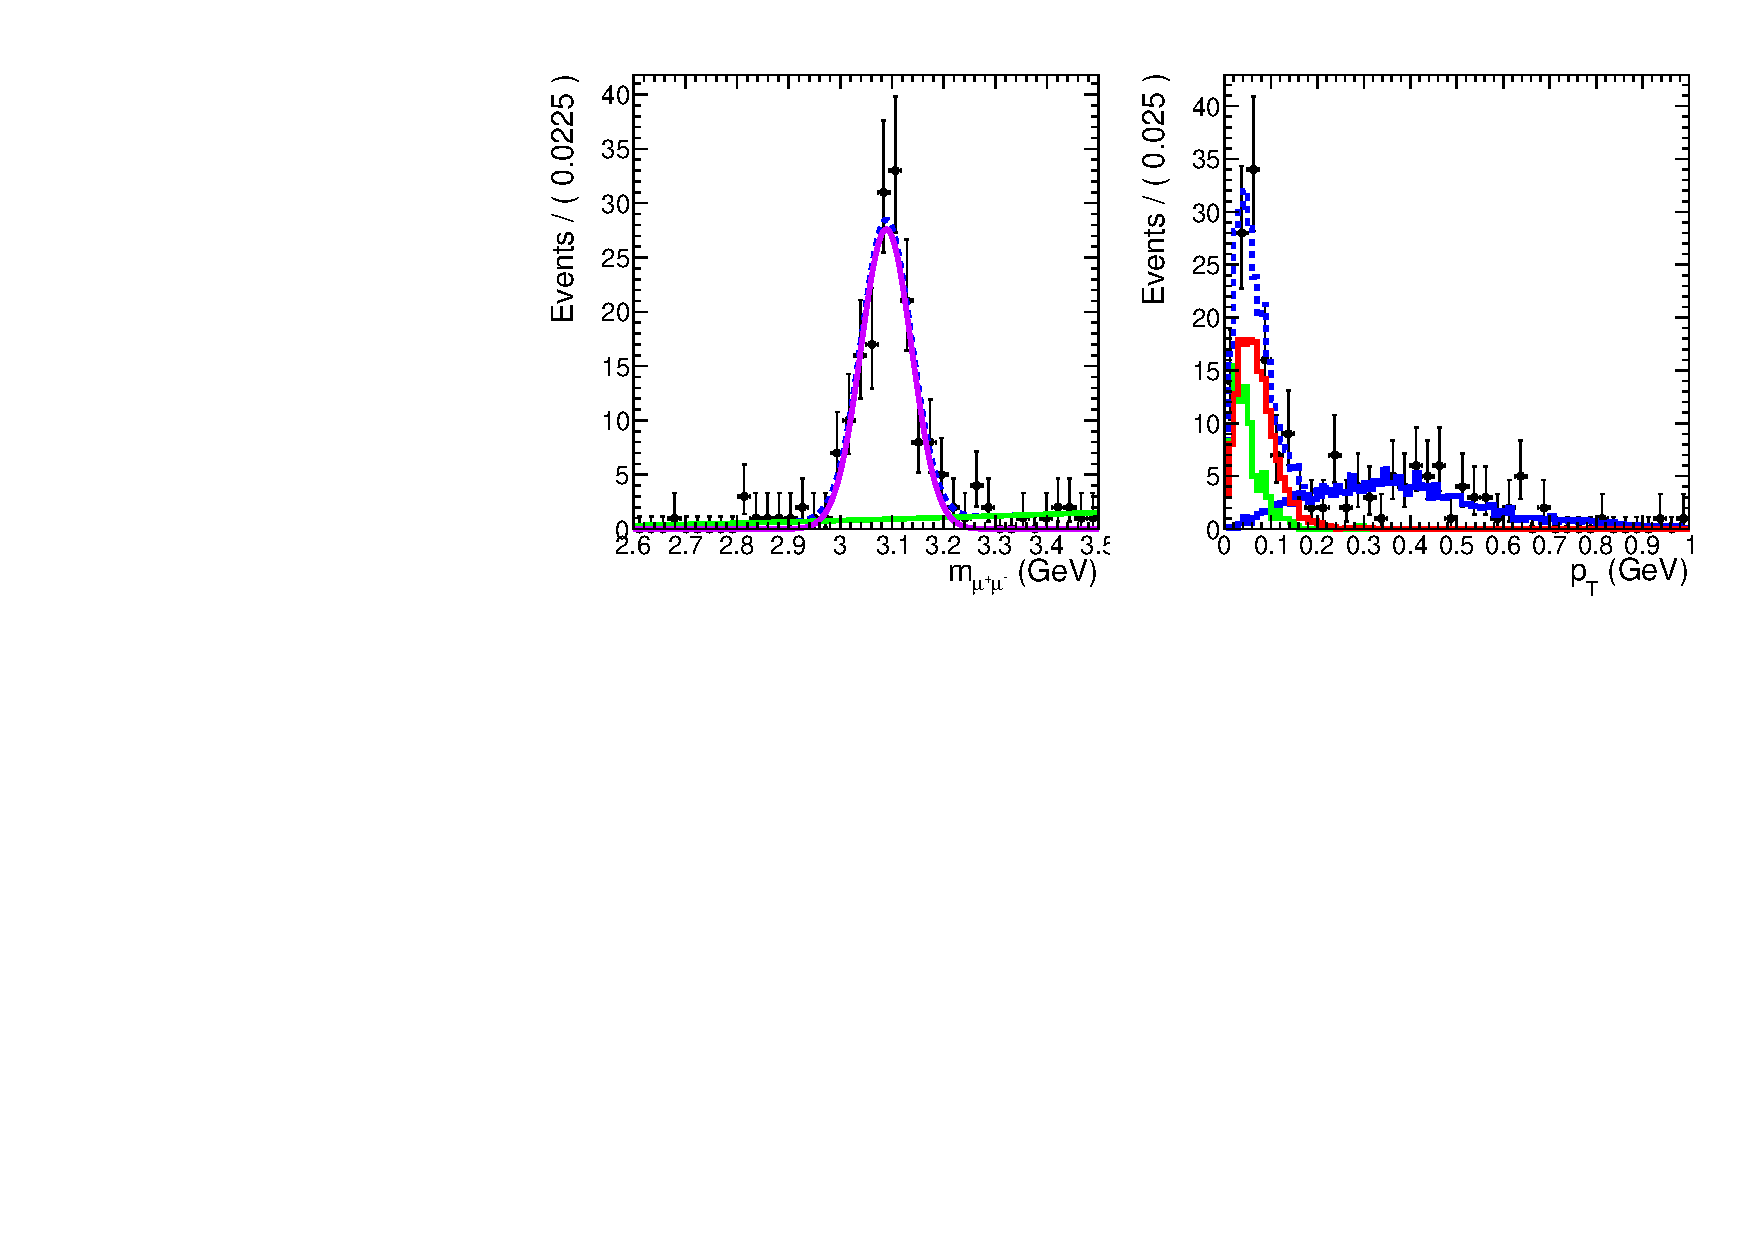
\includegraphics[width=0.9\textwidth]{ptMassSimGaussLine}
      \caption{Simultaneous fit to the mass and \pt{} spectra.}
      \label{fig:simFitMassPtGauss}
    \end{figure}

    Fig.~\ref{fig:simGaussCor} shows the confidence contours for $nCo$ and 
      $nGamma$ from the simultaneous fit in Fig.~\ref{fig:simFitMassPtGauss}.  
    The slope of the confidence contours in Fig.~\ref{fig:simGaussCor} 
      is noticeably than in Fig.~\ref{fig:ptOnlyCor}.
    The contours for the simultaneous fit are also reduced compared to 
      Fig.~\ref{fig:ptOnlyCor} with widths in $nCo$ and $nGamma$ similar to 
      those expected from Poison statistics. 
    From the simultaneous fit, reasonable statistical errors were obtained 
      along with the yields for the three processes. 

    \begin{figure}[!Hhbt]
      \centering
      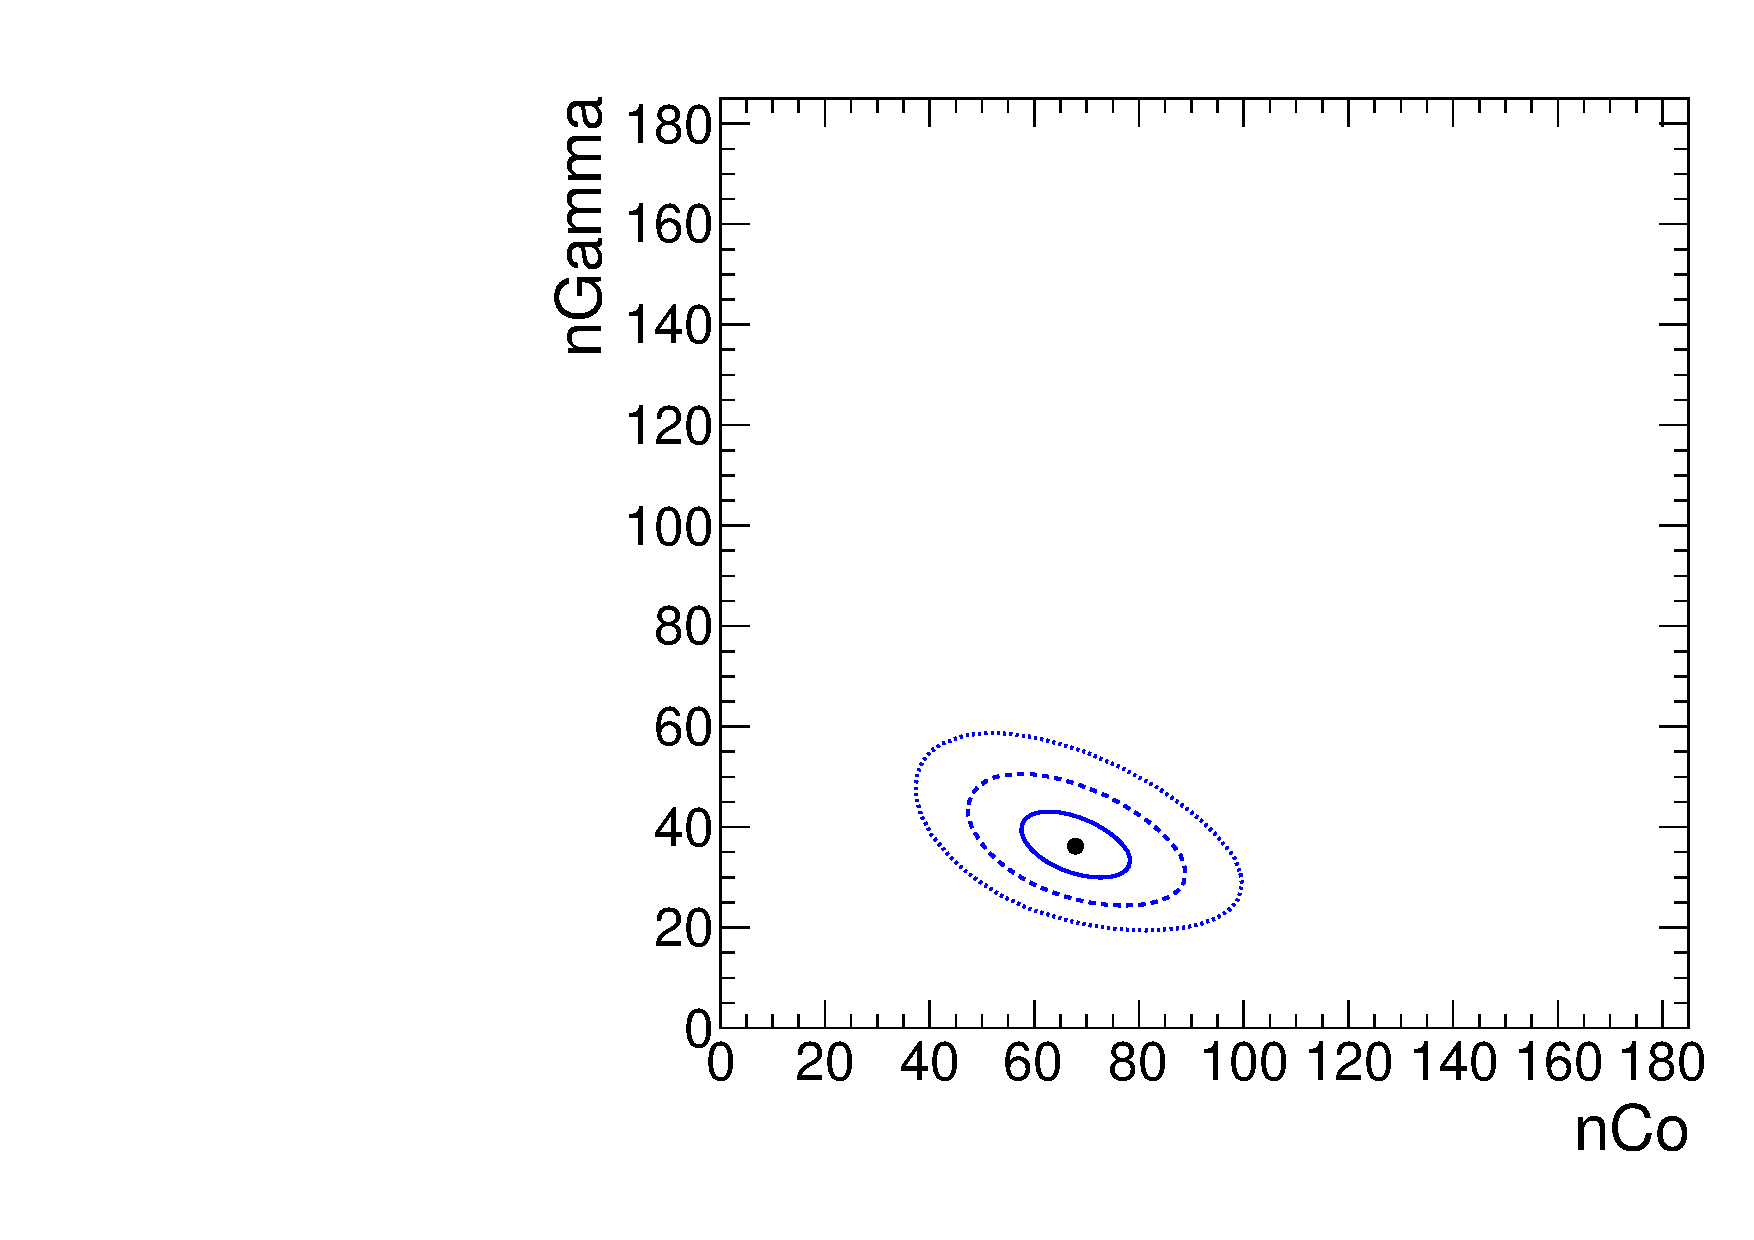
\includegraphics[width=0.6\textwidth]{nCoNGammaCorPtMass}
      \caption{68\%, 95\%, and 99\% confidence contours from the 
        simultaneous fit. }
      \label{fig:simGaussCor}
    \end{figure}

  \section{\label{sec:effDet} Efficiency determination}
    Each step of the triggering, event selection, and analysis has an associated
      efficiency that must be accounted for in the  measurement of the \JPsi{} 
      cross section.  
    The ZDC trigger efficiency, the muon trigger efficiency, and the muon 
      reconstruction efficiency are the two most significant contributors to 
      the total efficiency measurement. 
    The efficiency of the pixel track requirement, and the veto on activity in 
      the BSCs from the trigger are also estimated but found to be consistent 
      with fully efficient. 
    The following section explains how each of these efficiencies were measured
      with a special emphasis on the ZDC trigger efficiency and the muon 
      trigger and reconstruction efficiencies. 

    \subsection{Muon efficiencies}
      The muon efficiencies were measured using a combination of MC and data 
        based methods.
      The MC based measurement accounts for the detector acceptance and the 
        efficiency of the muon quality cuts discussed in 
        Section~\ref{sec:DataSetEvSel}.
      The trigger efficiencies were measured in data using the tag and probe 
      method \cite{cmsTnP}, which is discussed below. 

      CMS has a limited acceptance for \JPsi{}s, particularly in the case of 
        \JPsi{}s with low momentum like those produced in UPC events. 
      To measure the acceptance of CMS for \JPsi{}s, reconstructed dimuon 
        candidates were considered detectable if both reconstructed muon 
        daughters fell into a detectability region in \pt{} and $\eta$.
      The muon detectability region was defined using the coherent \JPsi{} 
        events obtained from STARlight.
      The efficiency for reconstructing single muons $\varepsilon^{\mu}_{reco}$ 
        is defined by $\varepsilon^{\mu}_{reco} = \frac{N^{\mu}_{reco}}{N^{\mu}_{gen}}$, 
        where $N^{\mu}_{reco}$ is the number reconstructed muons obtained 
        after the full CMS detector simulation and that passed the standard
        muon quality cuts, and $N^{\mu}_{gen}$ is the number of generated 
        muons from STARlight.
      \begin{figure}[!Hhtb]
        \centering
          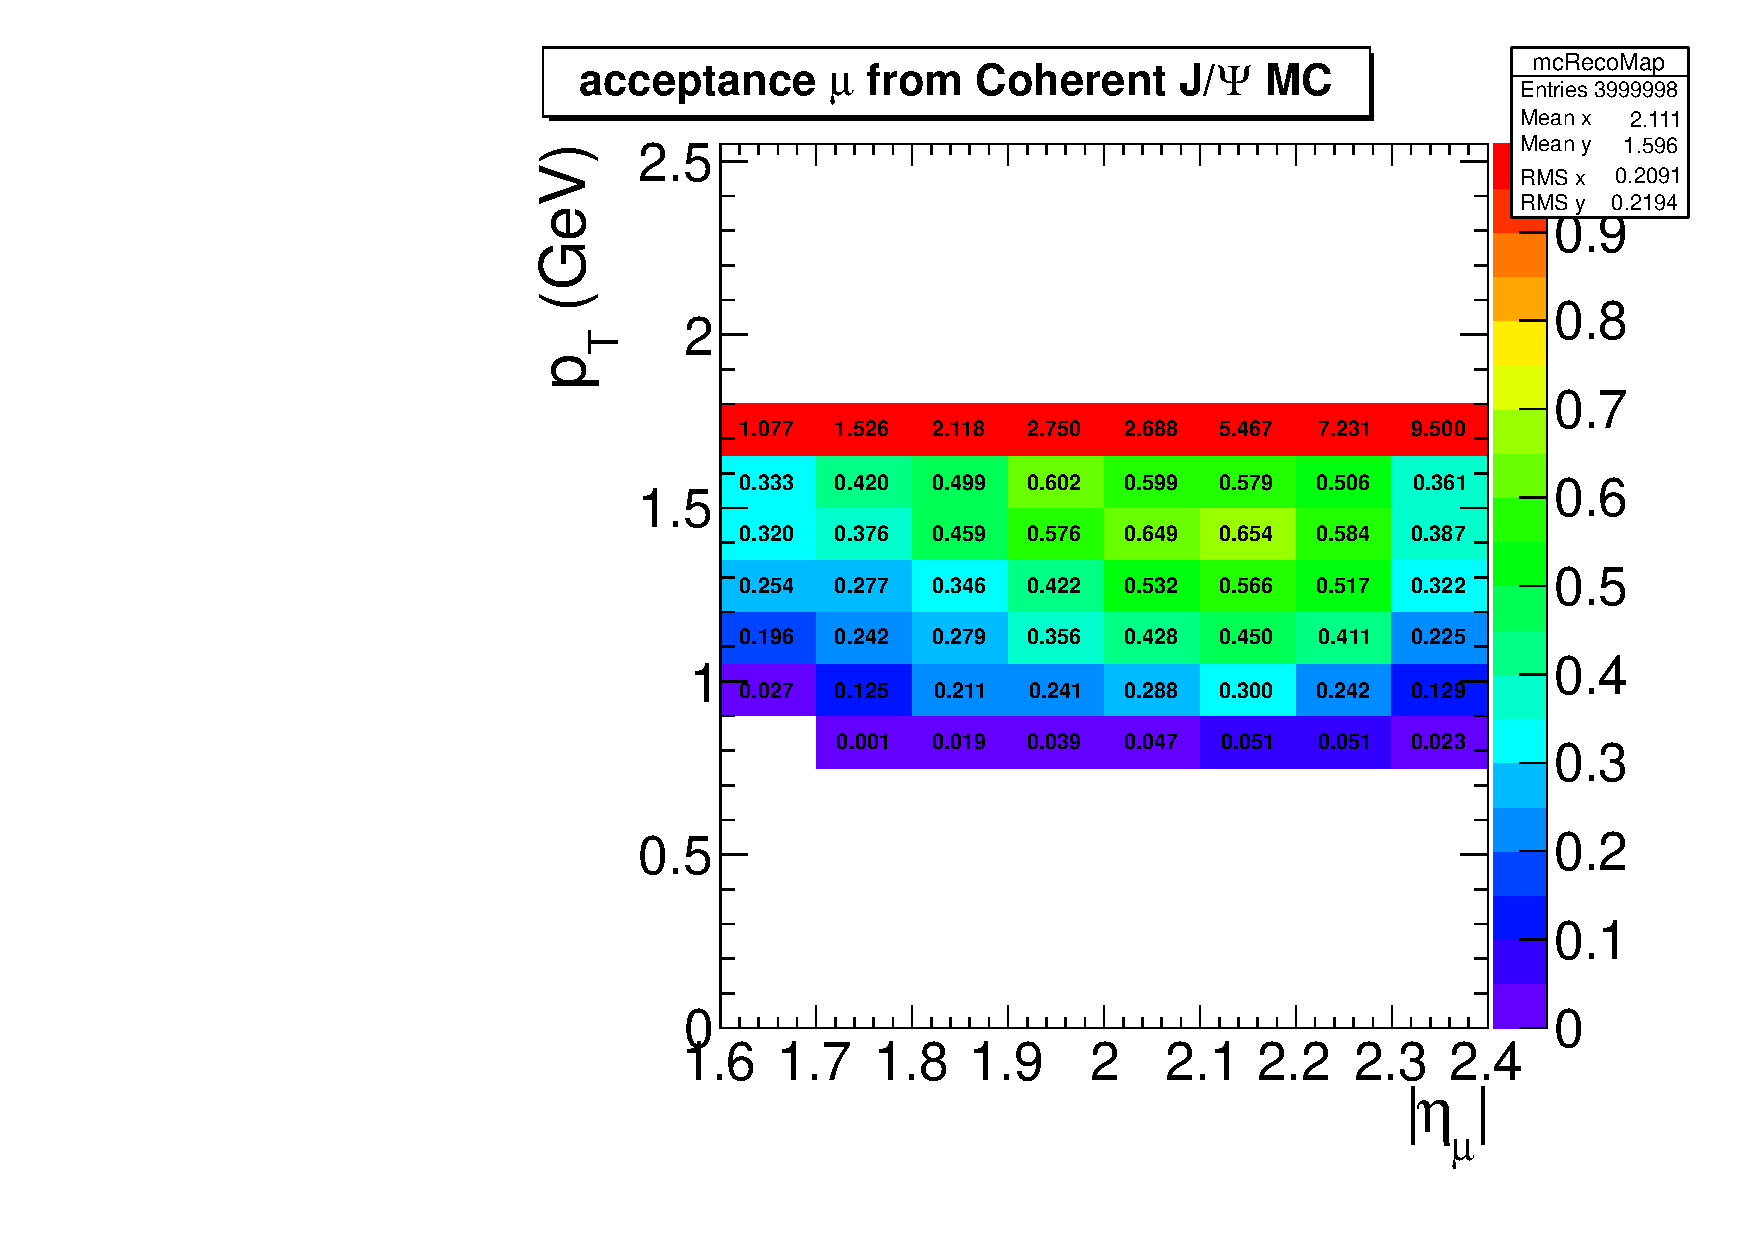
\includegraphics[width=.6\textwidth]{mcEffMaps/accMuJpCo} 
        \caption{ Muon daughter detectability from coherent \JPsi{}}
        \label{fig:muonDaughterDet}
      \end{figure}
      Fig.~\ref{fig:muonDaughterDet} shows the efficiency for reconstructing
        single muons from coherent \JPsi{} events.
      To avoid the edges of the detectors acceptance, all reconstructed muons 
        that fall into a (\pt{},$|\eta|$) bin that has an efficiency less 
        than 20\% were rejected.
      This condition defines the detectability region.
      The acceptance for reconstructing dimuons was calculated from MC
        using the following formula:
      \begin{equation}
        A=\frac{N_{det}(|y|,p_{T})}{N_{gen}(|y|,p_{T})},
        \label{eq:jpsiAccEq}
      \end{equation}
        where $N_{det}$ is the number of reconstructed dimuons where both 
        daughters fall into the detectability region, and $N_{gen}$ is the
        number of generated dimuons. 
      From Eq.~\ref{eq:jpsiAccEq}, the acceptance for \JPsi{} was calculated
        as a function of $|y|$, and \pt{} (see Fig.~\ref{fig:jpsiAcceptance}).
        \begin{figure*}[!Hhtb]
          \centering
          $ \begin{array}{cc}
            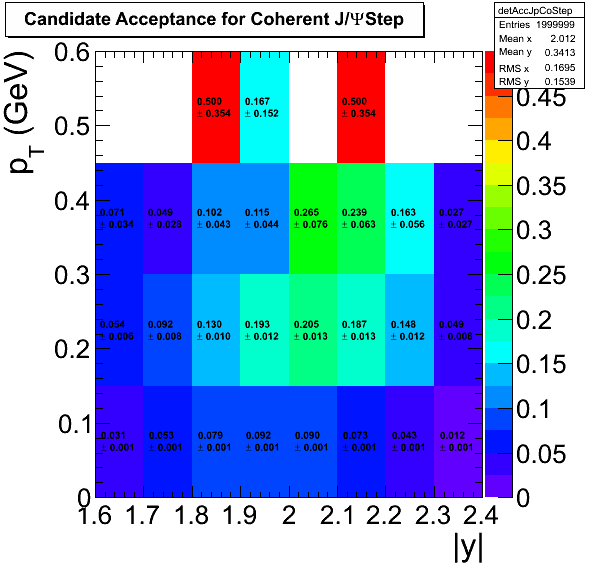
\includegraphics[width=.45\textwidth]{mcEffMaps/detAccJpCoStep} &
            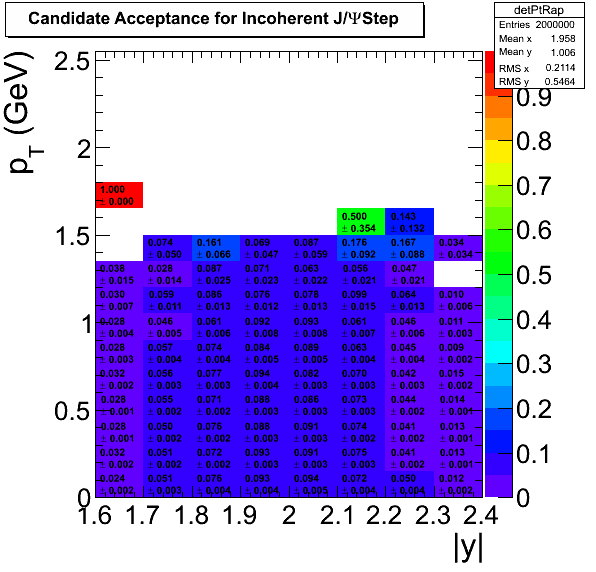
\includegraphics[width=.45\textwidth]{mcEffMaps/detAccJpInCoStep} \\
            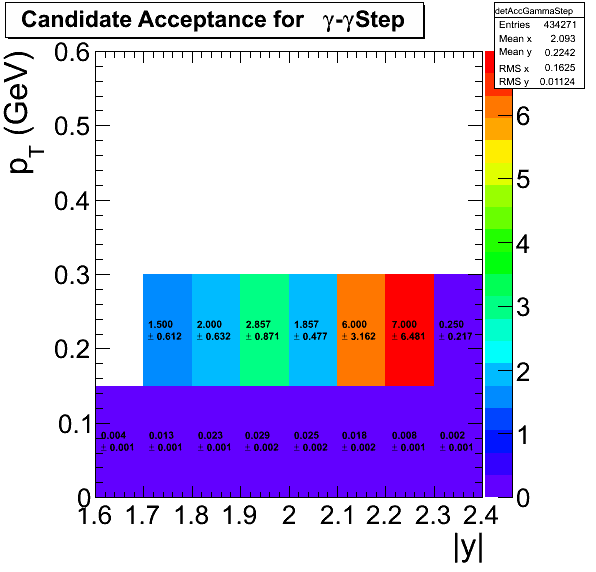
\includegraphics[width=.45\textwidth]{mcEffMaps/detAccGammaStep}
          \end{array} $
          \caption{Dimuon acceptance from coherent \JPsi{} (top left), incoherent 
            J$\psi$ (top right), and photon-photon interactions (lower).}
          \label{fig:jpsiAcceptance}
        \end{figure*}

      The "tag and probe method" is a data driven approach used to measure the 
        trigger efficiency of the muon daughters from \JPsi{} decays.
      In this method there are three categories of daughter muons. 
      \textit{Tag muons} are high quality muons.
      \textit{Passing probes} are reconstructed muons that match the muon 
        trigger, while \textit{failing probes} do not. 
      Each dimuon will have one daughter classified as a tag and the other
        as a probe.
      From here three invariant mass histograms are studied. 
      One histogram is created from all pairs. 
      The second comes from pairs where the probe is a passing probe.  
      The last histogram comes from pairs where the probe fails to fulfill
        the trigger, \DIFdelbegin \textit{\DIFdel{i.e.}} %DIFAUXCMD
\DIFdel{the probe }\DIFdelend \DIFaddbegin \DIFadd{it }\DIFaddend is a failing probe. 
      By matching the tag to the trigger, the probe is unbiased by the trigger 
        and the  efficiency can be measured by fitting the three mass 
        histograms. 

      Because the trigger efficiency depends on the \pt{} and $|\eta|$ of the 
        muon, one set of three histograms for each (\pt{},$|\eta|$) bin of the
        probe is created.
      To extract the single muon trigger efficiency $\varepsilon^{\mu}_{trig}$, 
        each set of invariant mass histograms were simultaneously fit. 
      The signal was \DIFdelbegin \DIFdel{fitted }\DIFdelend \DIFaddbegin \DIFadd{fit }\DIFaddend using a Crystal Ball function, and the background 
        was \DIFdelbegin \DIFdel{fitted }\DIFdelend \DIFaddbegin \DIFadd{fit }\DIFaddend to an exponential.
      The Crystal Ball parameters were simultaneously \DIFdelbegin \DIFdel{fitted }\DIFdelend \DIFaddbegin \DIFadd{fit }\DIFaddend to all three 
        histograms.
      The exponential function was \DIFdelbegin \DIFdel{fitted }\DIFdelend \DIFaddbegin \DIFadd{fit }\DIFaddend to the failing and passing probe 
        histograms separately.
      Because the background shapes are in principle different for the two 
        samples, the efficiency is driven by this difference. 

      Fig.~\ref{fig:tnpFitPlot} shows the fit of the three sets of pairs. 
      \begin{figure}[!Hh]
        \centering
        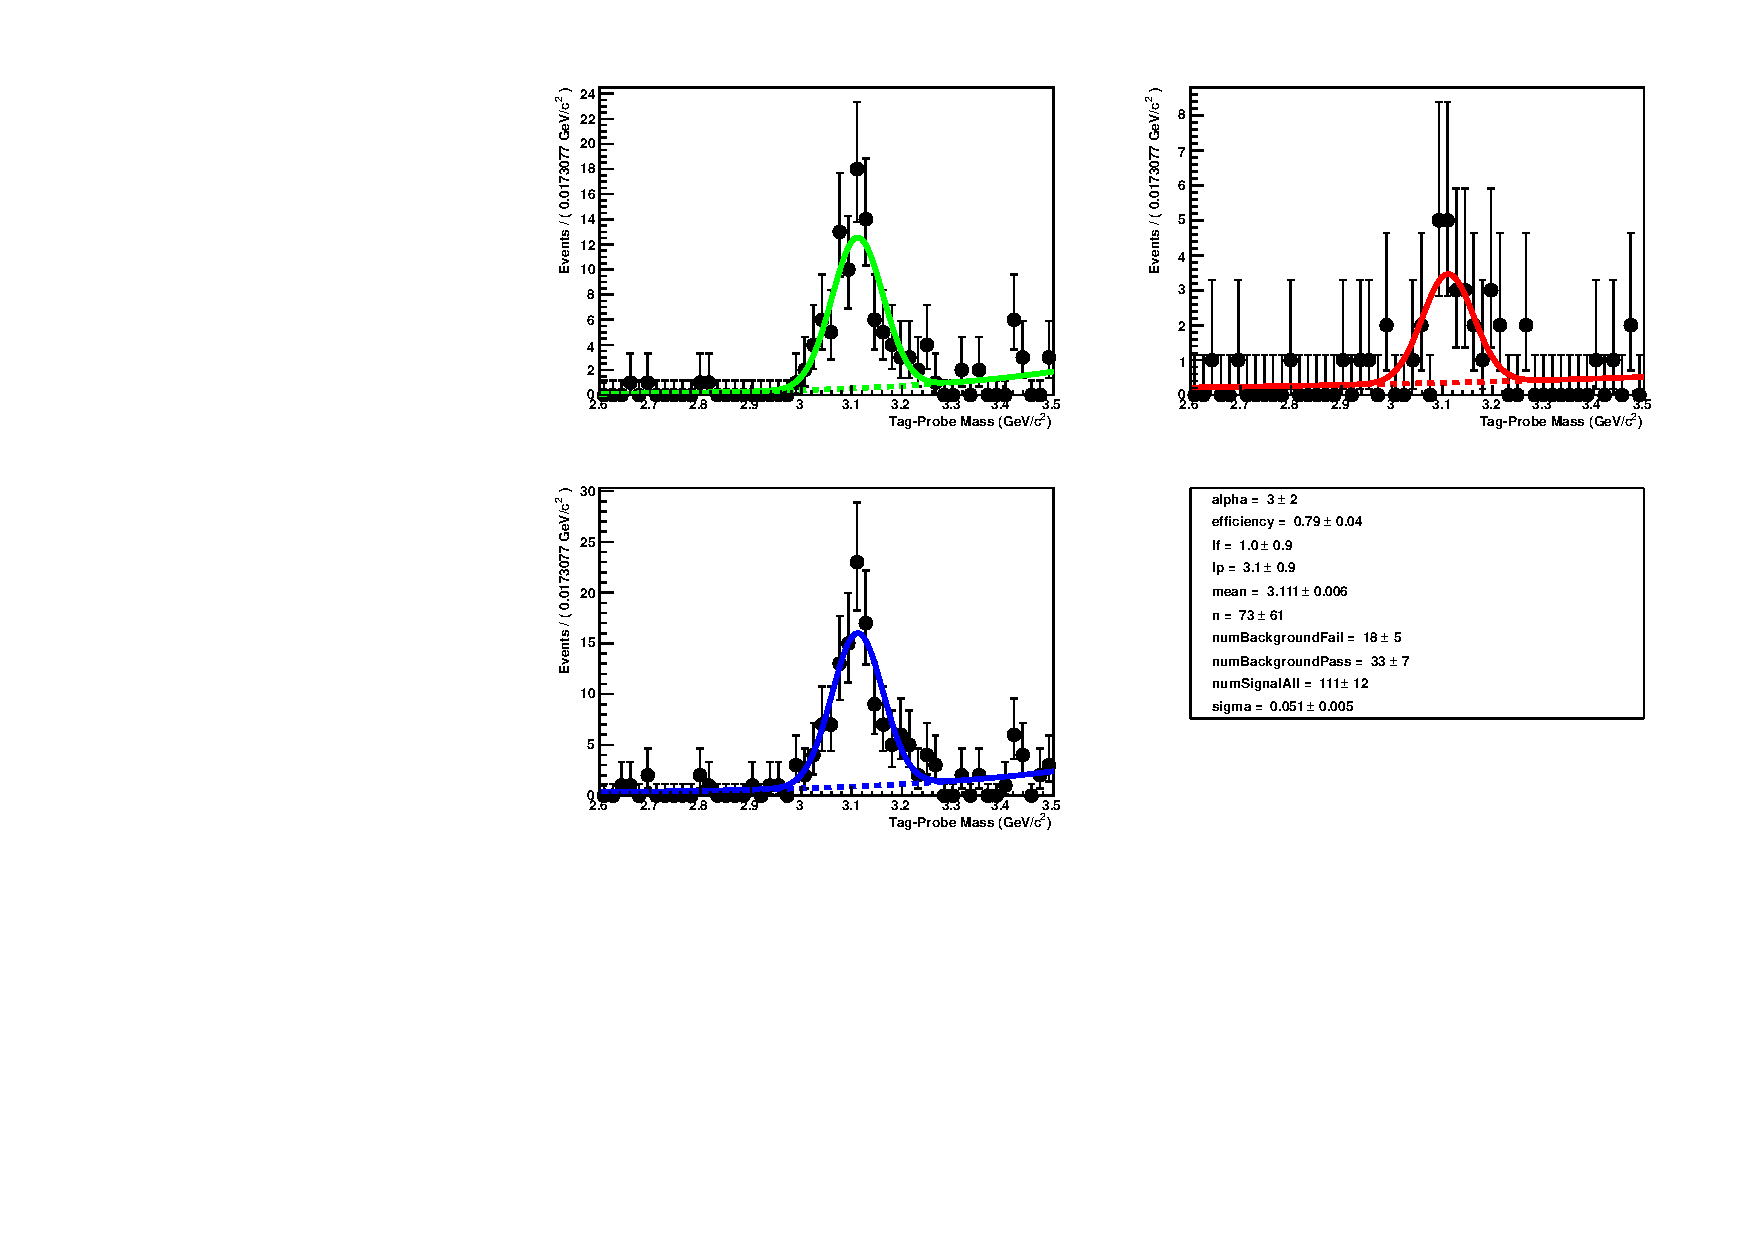
\includegraphics[width=.6\textwidth]{tNp/tnpFits}
        \caption{Fits to tag and probe pairs in the \JPsi{} mass region for
        pairs with a probe 2 < |$\eta$| < 2.2 and 1.55 < \pt{} < 1.8 GeV.}
        \label{fig:tnpFitPlot}
      \end{figure}
      This fit was done for each bin of the probes \pt{} and $\eta$.
      The efficiency from the fits in each bin are shown in Fig.~\ref{fig:tnpTrigMap}.
      \begin{figure}[!Hhbt]
        \centering
        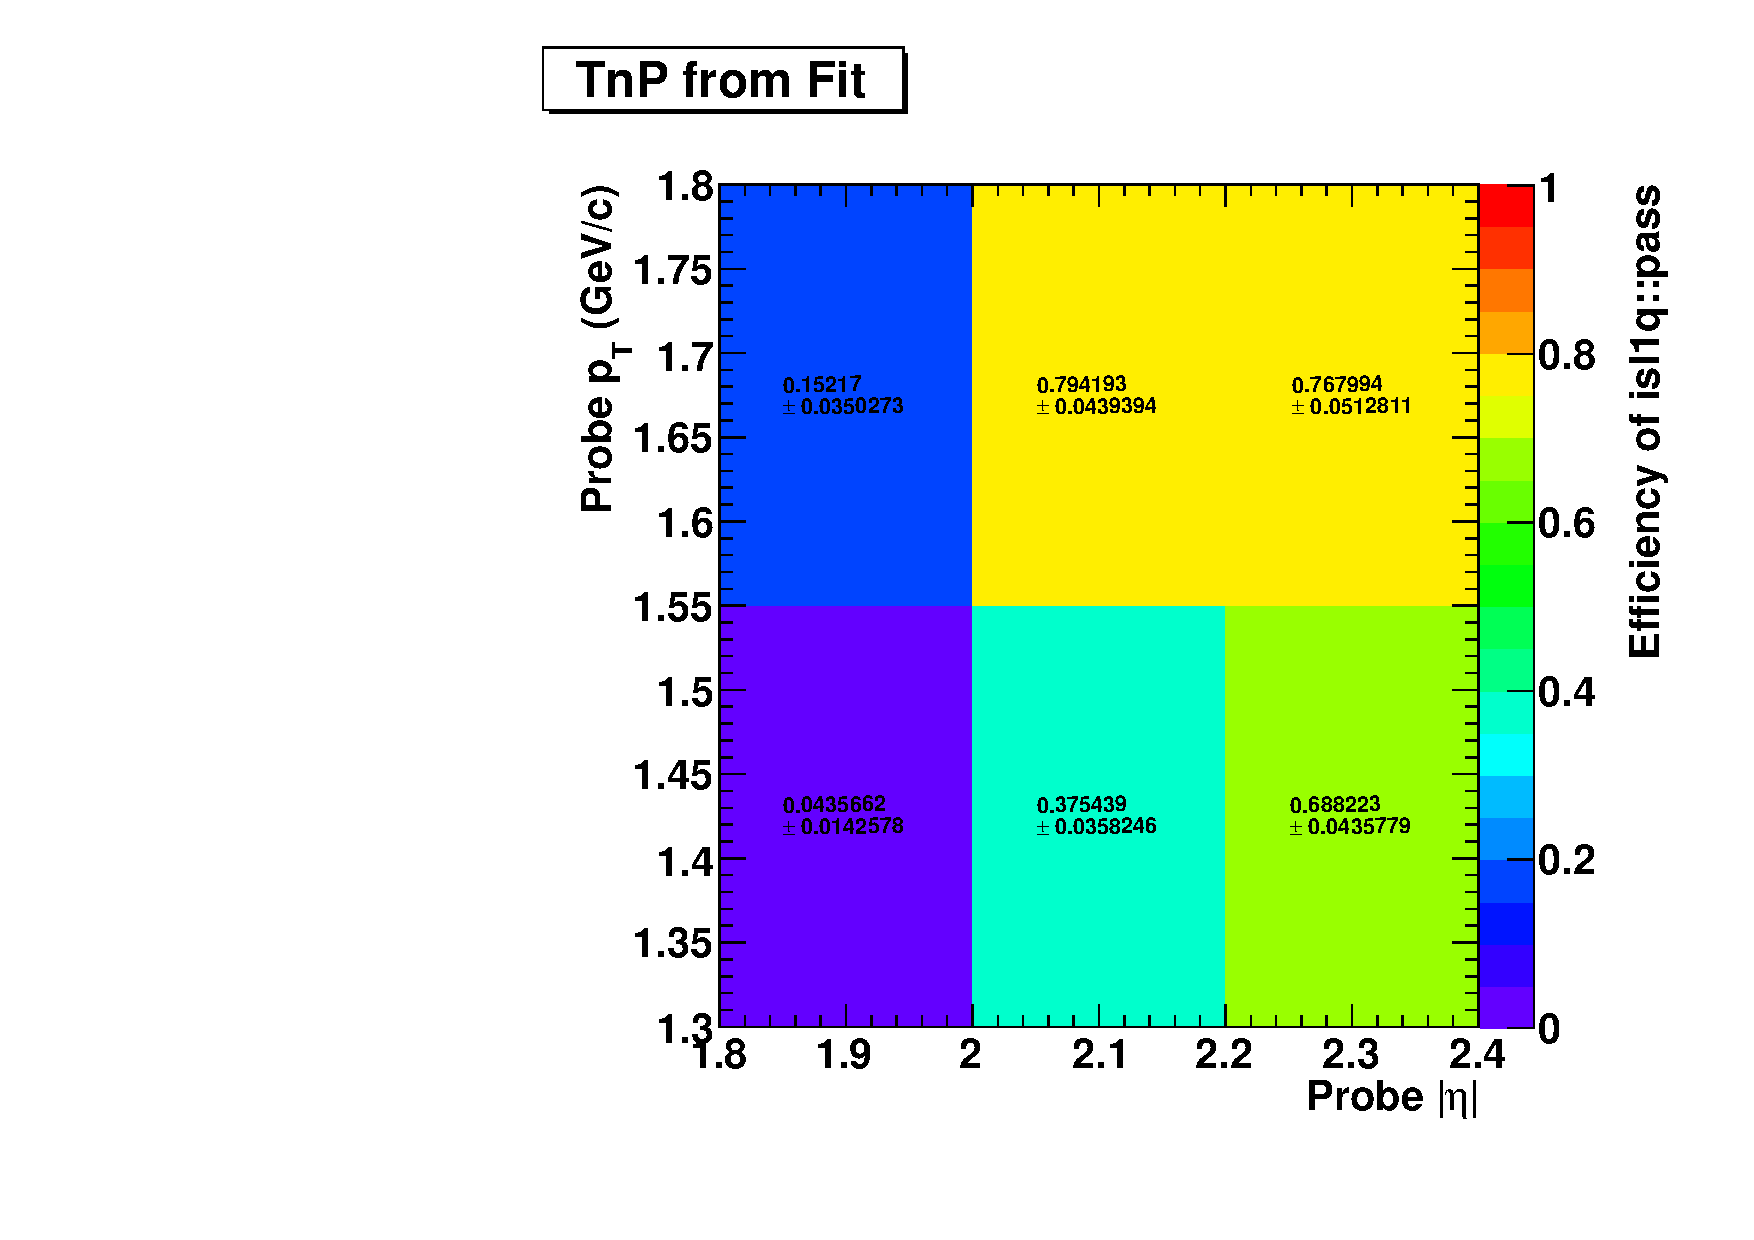
\includegraphics[width=.6\textwidth]{tNp/tnpFromFit}
        \caption{Muon trigger efficiencies in \pt{} and $\eta$ bins from 
          the tag and probe method.}
        \label{fig:tnpTrigMap}
      \end{figure}

      The dimuon trigger efficiency $\varepsilon^{dimuon}_{trigger}$ was 
        calculated from the single muon efficiencies using the following
        equation:
      \begin{equation}
        \label{eq:dimuTrigEff}
        \varepsilon^{dimuon}_{trigger}=1-(1-\varepsilon_{trigger}^{\mu_{1}})(1-\varepsilon_{trigger}^{\mu_{2}}),
      \end{equation}
      where $\varepsilon_{trigger}^{\mu_{1}}$ is the tag and probe efficiency
        of the first dimuon daughter, and $\varepsilon_{trigger}^{\mu_{2}}$ is
        the efficiency of the second muon daughter. 
      In Eq.~\ref{eq:dimuTrigEff} the probability of at least one daughter
        firing the trigger is calculated by subtracting one from the
        probability that neither daughter fires the trigger,
        thus giving the dimuon trigger efficiency. 

      The average dimuon trigger efficiency for each dimuon (\pt{},$|y|$) bin
        was calculated by averaging the efficiency of dimuon candidates in each
        bin. 
      \begin{figure}[!Hhbt]
        \centering
        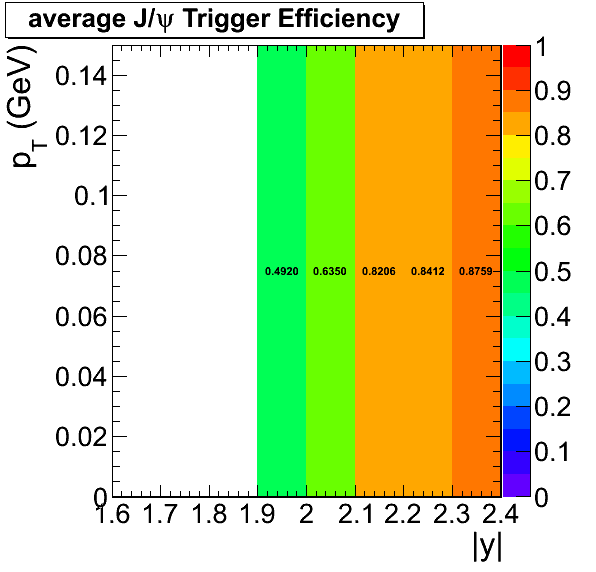
\includegraphics[width=0.6\textwidth]{averageTriggerEff}
        \caption{The trigger efficiency from tag and probe averaged over candidates
          in each (\pt{},$|y|$) bin.}
        \label{fig:avTrigEffCo}
      \end{figure}
      The dimuon trigger efficiency ranges from \DIFdelbegin \DIFdel{$\approx 50$\% to 87}\DIFdelend \DIFaddbegin \DIFadd{about 50\% to 90}\DIFaddend \%. 
      As expected the \JPsi{} trigger efficiency increase with rapidity since 
        the longitudinal momentum of the \JPsi{} is given 
        $p_Z= M_{J/\psi} \cdot sinh(y)$. 
      Thus \JPsi{} mesons at forward rapidity distribute more momentum to their
        daughter muons which therefore have a greater chance of punching 
        through into the muon chamber.  
      The average trigger efficiency was multiplied by the acceptance and 
        reconstruction efficiency from the MC to produce a total factor for 
        both efficiency and acceptance. 
      \begin{figure}[!Hhtb]
        \centering
        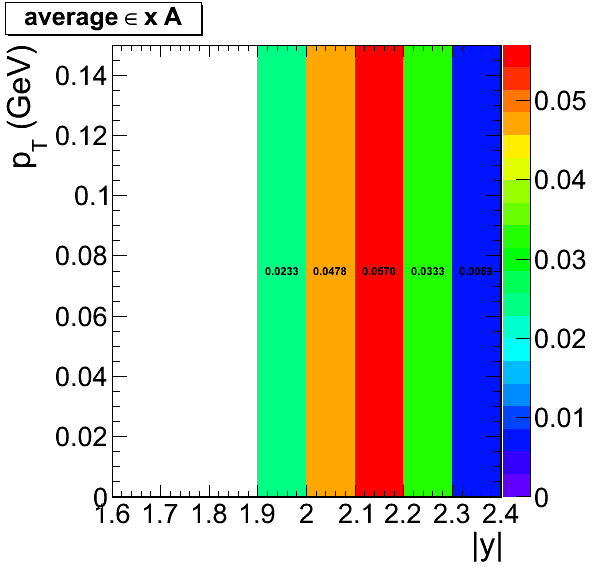
\includegraphics[width=0.6\textwidth]{averageExA}
        \caption{The acceptance times averaged trigger efficiency from tag and 
          probe.}
        \label{fig:avAccEff}
      \end{figure}

      The total combined efficiency and acceptance factor coherent \JPsi{} 
        between $2.0 \le |y| \le 2.2$ was found to be $\approx 5$\%.
      The acceptance factor of roughly 7\% from the MC was found to be the main
        contributor to the total efficiency. 
      The interplay of the polarization of the \JPsi{} and the material in 
        detector drive down the efficiency by creating an effective momentum 
        threshold for detection (see Section~\ref{sec:mcSim}).
      The reconstruction efficiency of the daughters range between 
        20\%-60\% for muons in the defined detectability range. 
      The trigger efficiency for the detectable muons ranges from 30\%-80\% 
        depending on \pt{}. 

    \subsection{ZDC trigger efficiency}
      As discussed in Section~\ref{sec:breakUpDet}, the trigger labeled 
        "L1ZDCOr and Pixel Track" in Table~\ref{tab:hltTriggers2011} was used 
        to measure the ZDC trigger efficiency. 
      This trigger required either a ZDC$^{+}$ or ZDC$^{-}$ trigger, together with at 
        least one pixel track. 
      The veto on the BSC minimum bias trigger, as in the physics triggers, was
        applied offline.
      The BSC veto excludes events where BSCs from both sides of the 
        interaction point are above threshold. 
      This trigger was used in order to collect the most inclusive possible 
        sample without using the minimum bias triggers designed to collect 
        hadronic interactions.

      This ZDC triggered sample suffers from a trigger bias. 
      For example, a sample triggered by ZDC$^{+}$ would always produce a 
        ZDC$^{+}$ trigger efficiency of one. 
      To avoid this, a similar technique to tag and probe was used.
      Each event is either tagged as triggered by ZDC$^{+}$ or triggered 
        by the ZDC$^{-}$. 
      The ZDC$^{+}$ trigger efficiency is measured from the ZDC$^{-}$ tagged 
        sample, and vice versa.

      To estimate the efficiency, the number of events with energy in 
        ZDC$^{+}$ greater than the single neutron threshold, N$_{events}$, 
        was measured.
      From this set of events, the number of events that also fire the 
        ZDC$^{+}$, N$_{trig}$, was measured.
      The ratio between the number of single neutron events that fired the 
        trigger and all single neutron events was taken as the estimate of 
        trigger efficiency. 
      The same procedure was applied for each side of the ZDC.
      The trigger efficiency was found to be 98\% for ZDC$^{-}$
        and 94\% for ZDC$^{+}$.

      \begin{table}
        \centering
        \begin{tabular}{|c|c|c|c|c|}
           \hline ZDC Side & N$_{events}$ & N$_{trig}$ & $\varepsilon_{ZDC}$ \\ \hline
           ZDC$^{+}$ & 73028  & 71706  & 0.9819  $\pm$ 0.005  \\ \hline
           ZDC$^{-}$ & 76132  & 71859  & 0.9439  $\pm$ 0.005  \\ \hline
        \end{tabular}
        \caption{ZDC trigger efficiencies for ZDC reconstruction method 1 and 
          2}
        \label{tab:zdcEfficiency}
      \end{table}

  \section{\label{sec:sysCheck}Systematic \DIFdelbegin \DIFdel{checks}\DIFdelend \DIFaddbegin \DIFadd{uncertainties}\DIFaddend }

    Table~\ref{tab:sumsyst} shows the systematic errors that were estimated.
    The method used to separate the coherent from the photon-photon process 
     is the most dominant error.
    The ZDC reconstruction method used to estimate the neutron thresholds 
      is the next most dominant, followed by the method used to estimate
      the HF noise threshold. 
    \DIFdelbegin %DIFDELCMD < 

%DIFDELCMD <     %%%
\DIFdelend \begin{table}[!Hhtb]
      \begin{center}
        \begin{tabular}{|c|c|c|}
          \hline
          systematic & uncertainty in \%  \\ \hline
          Template fit \DIFdelbeginFL \DIFdelFL{normalized }\DIFdelendFL \DIFaddbeginFL \DIFaddFL{normalization }\DIFaddendFL & +9.5\% -12\%    \\ \hline
          ZDC trigger efficiency & 2.2\%    \\ \hline
          ZDC reconstruction  & 2.9\%  \\ \hline
          HF noise threshold & +1.3\% -3.4\%    \\ \hline 
          MC acceptance & 1.1\%    \\ \hline
          \hline \hline
          Total systematic & 8.1\%    \\ \hline
        \end{tabular}
        \caption{Summary of systematic uncertainties}
        \label{tab:sumsyst}
      \end{center}
    \end{table}

    \subsection{HF noise threshold}
      The way in which the HF noise distribution is measured effects the event 
        selection and therefore the final candidate \DIFdelbegin \DIFdel{yeild}\DIFdelend \DIFaddbegin \DIFadd{yield}\DIFaddend .
      This cut plays a significant role in rejecting hadronic events.
      In Table~\ref{tab:evSelCutNumbers} the importance of cutting on HF noise
        is evident. 
      The HF noise cut rejects nearly 1/5 of the remaining events. 
      The systematic uncertainties on the HF noise requirement is important for
        this reason.

      The most fine grained data from the HF detectors are called RecHits. 
      There is one RecHit per phototube on HF. 
      The RecHit signal is calibrated in GeV, and no noise subtraction is done. 
      The CaloTowers are formed from geometrical groups of RecHits. 
      They are the first stage of the CMS jet trigger and perform some noise 
        suppression.

      The default HF noise cut required that the maximum RecHit energy
        from both HF+ and HF- be less than 3.85 GeV. 
      This cut was designed to accept 99\% of the noise events, 
        see Fig.~\ref{fig:hfNoiseDist}. 
      The stability of this cut was tested by
      \begin{enumerate}
        \item Summing CaloTowers instead of RecHits
        \item Making separate cuts on HF- and HF+
        \item Tightening the threshold so that only 98\% or 97\% noise events 
          passed the cut.
      \end{enumerate}

      Table~\ref{tab:hfNoiseThreshAsym} shows the noise thresholds for RecHits 
        and CaloTowers for both the combined HF+ and HF- calorimeters and the 
        individual calorimeters when 99\% of noise events are accepted.
      Table~\ref{tab:hfAdjThreshYields} compares the threshold for the cases 
        when 99\%, 98\% and 97\% of noise events are accepted.
      The number of J$/\psi$ events remaining after these cuts is shown in 
        EXPANDED TABLE. 
      The efficiency corrected numbers are also shown. 
      The fractional systematic error is then estimated by finding the maximum 
        and minimum deviation from the default method. 
      The systematic uncertainty from this method is calculated to be +1.3\% 
        -3.4\%.

      \begin{table}[!Hhbt]
        \centering
        \begin{tabular}{|c|c|c|c|}
          \hline
          Object type & HF (GeV) & HF$^{-}$ (GeV) & HF$^{+}$ (GeV) \\ \hline
          RecHits & 3.85 & 3.25 & 3.45 \\ \hline
          CaloTowers & 4.25 & 3.25 & 3.75 \\ \hline
        \end{tabular}
        \caption{HF noise theresholds for various noise measurement methods.}
        \label{tab:hfNoiseThreshAsym}
      \end{table}

      \begin{table}[!Hhbt]
        \centering
        \begin{tabular}{|c|c|c|}
          \hline
          Object type & Combinded HF threshold & Two-sided thresholds \\ \hline
          RecHits & 298 & 290 \\ \hline
          CaloTowers & 302 & 288 \\ \hline
        \end{tabular}
        \caption{Candidate yields below 1.05 GeV \pt{} for various HF noise
          cuts.}
        \label{tab:hfCutYieldEffects}
      \end{table}

      \begin{table}[!Hhbt]
        \begin{center}
          \caption{Values of the energy cuts for the HF calorimeter for RecHit and CaloTower in GeV.}
          \label{tab:hfAdjustedThresholds}
          \begin{tabular}{|c|c|c|} \hline
            \% &  $E_{RecHit}$ GeV & $E_{CaloTower}$ GeV\\ 
            \hline
            99 & 3.85& 4.25 \\ \hline
            98 & 3.25& 3.75 \\ \hline
            97 & 2.95& 3.25 \\  \hline
           \end{tabular}
         \end{center}
      \end{table}

      \begin{table}[!Hhbt]
        \begin{center}
          \caption{Number of dimuon candidates with  p$_{T} <$1.05 when changing HF calorimeter cuts for RecHit and CaloTower.}
          \label{tab:hfAdjThreshYields}
          \begin{tabular}{|c|c|c|} \hline
            \% &  RecHit cut & CaloTower cut\\ \hline
            99 &   298 & 302 \\ \hline
            98 &  287  & 294 \\ \hline
            97 & 284 & 280 \\ \hline
          \end{tabular}
        \end{center}
      \end{table}

    \subsection{Template fit normalization}
      \begin{figure}[!Hhtb]
        \centering
        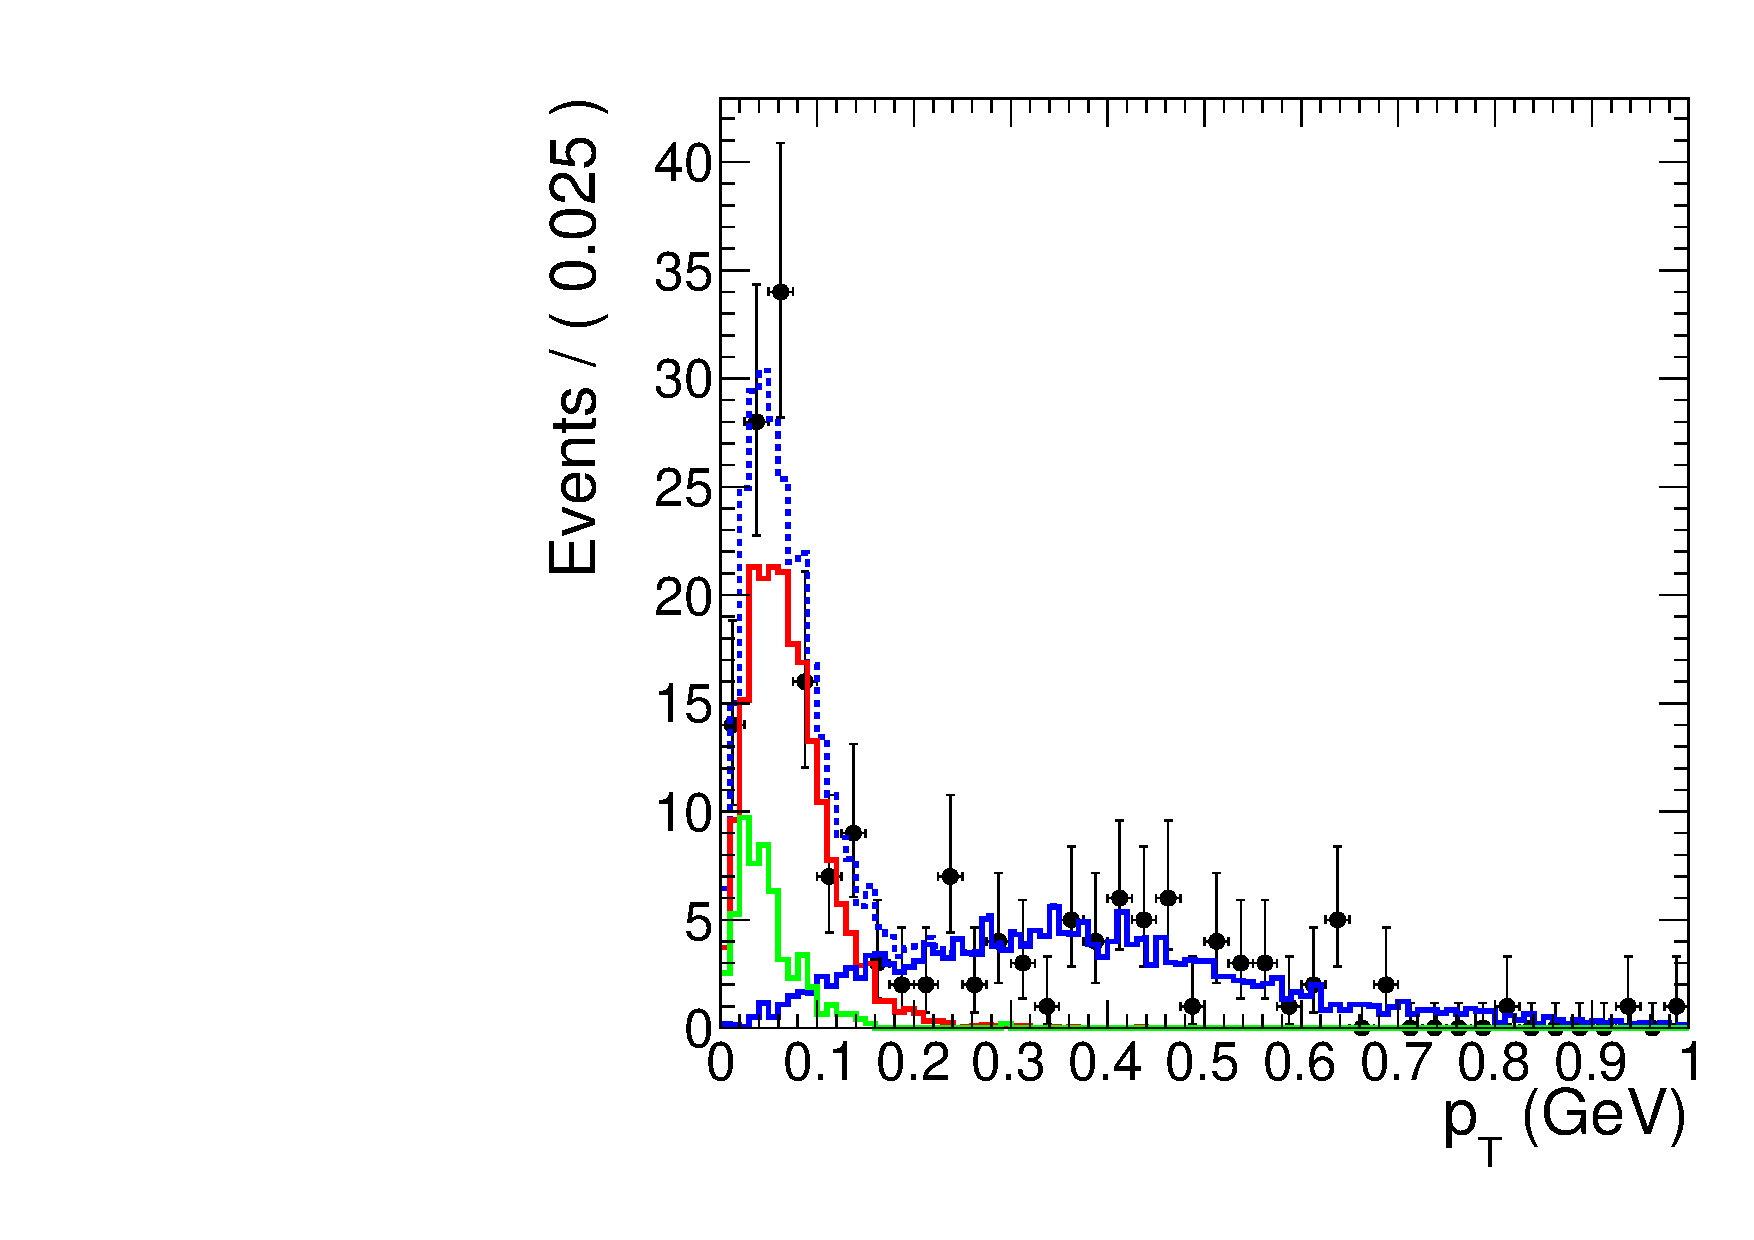
\includegraphics[width=.6\textwidth]{ptOnly}
        \caption{Coherent, incoherent, and photon-photon process \pt{} template fit to data.}
        \label{fig:ptTempFit}
      \end{figure}

      The \pt{} template fit depends on the functions chosen for the fit
        to the mass distribution.
      As described in Section~\ref{sec:sigEx}, the similarity of the of the 
        \pt{} distribution for the coherent and photon-photon process make
        the contributions from the two process difficult to separate from the 
        \pt{} distribution alone.
      The mass distribution was used to distinguish between these two processes.
      In turn, the \pt{} becomes dependent on the mass fit. 

      The systematic uncertainty due to the choose of functions used to fit
        the mass distribution was estimated by varying the signal and 
        background functions.
      The contribution to the background from the mass fit was used to fix the
        contribution from the photon-photon process in the \pt{} template
        fit.
      Two functions were used to describe the signal, a Gaussian, and a Crystal
        ball function. 
      The background was fit to a linear function, a 2nd order polynomial, and
        a 2nd order Cheby-Chev polynomial. 
      The resulting variation on the coherent contribution was used to as an
        estimate of this systematic effect. 

      \begin{figure}[!Hhbt]
        \centering
        $ \begin{array}{ccc}
          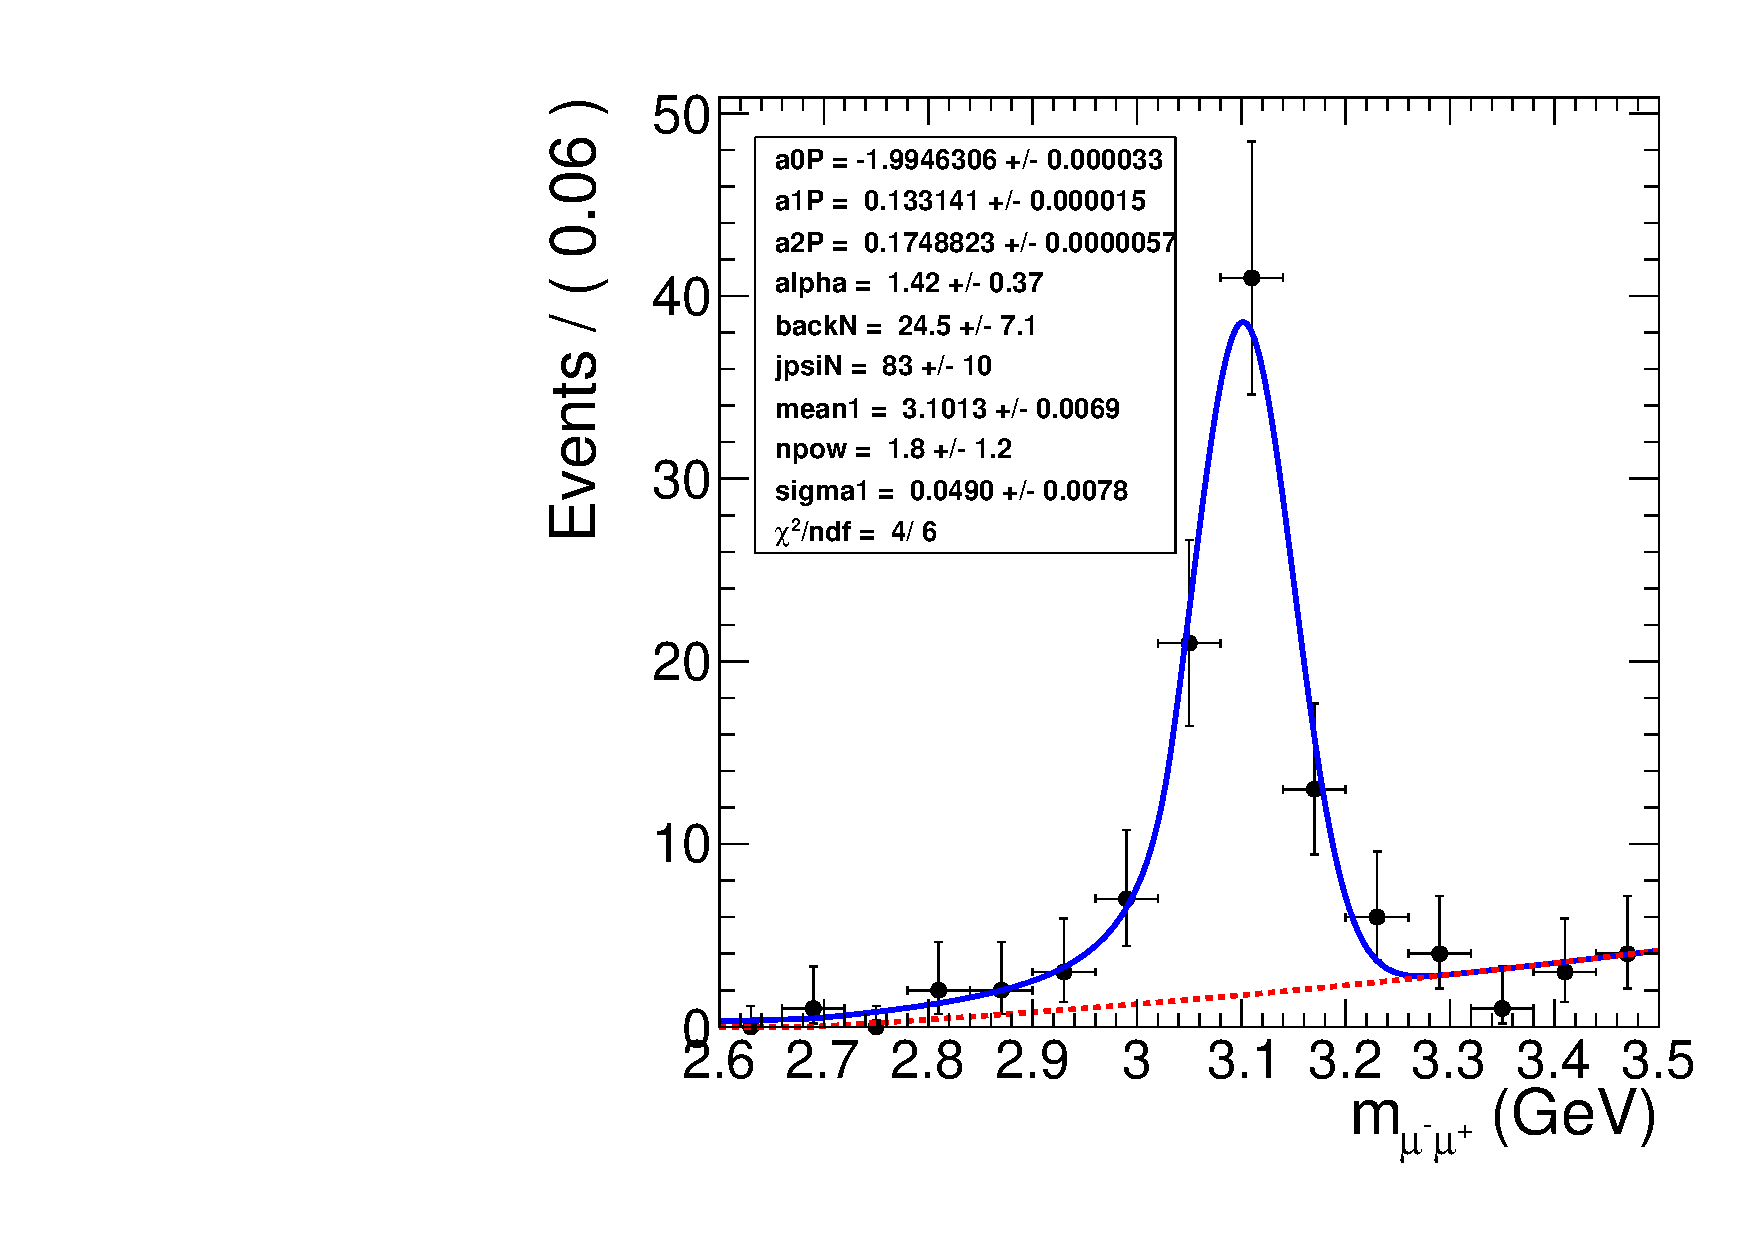
\includegraphics[width=.3\textwidth]{cbPolyBkgEst} &
          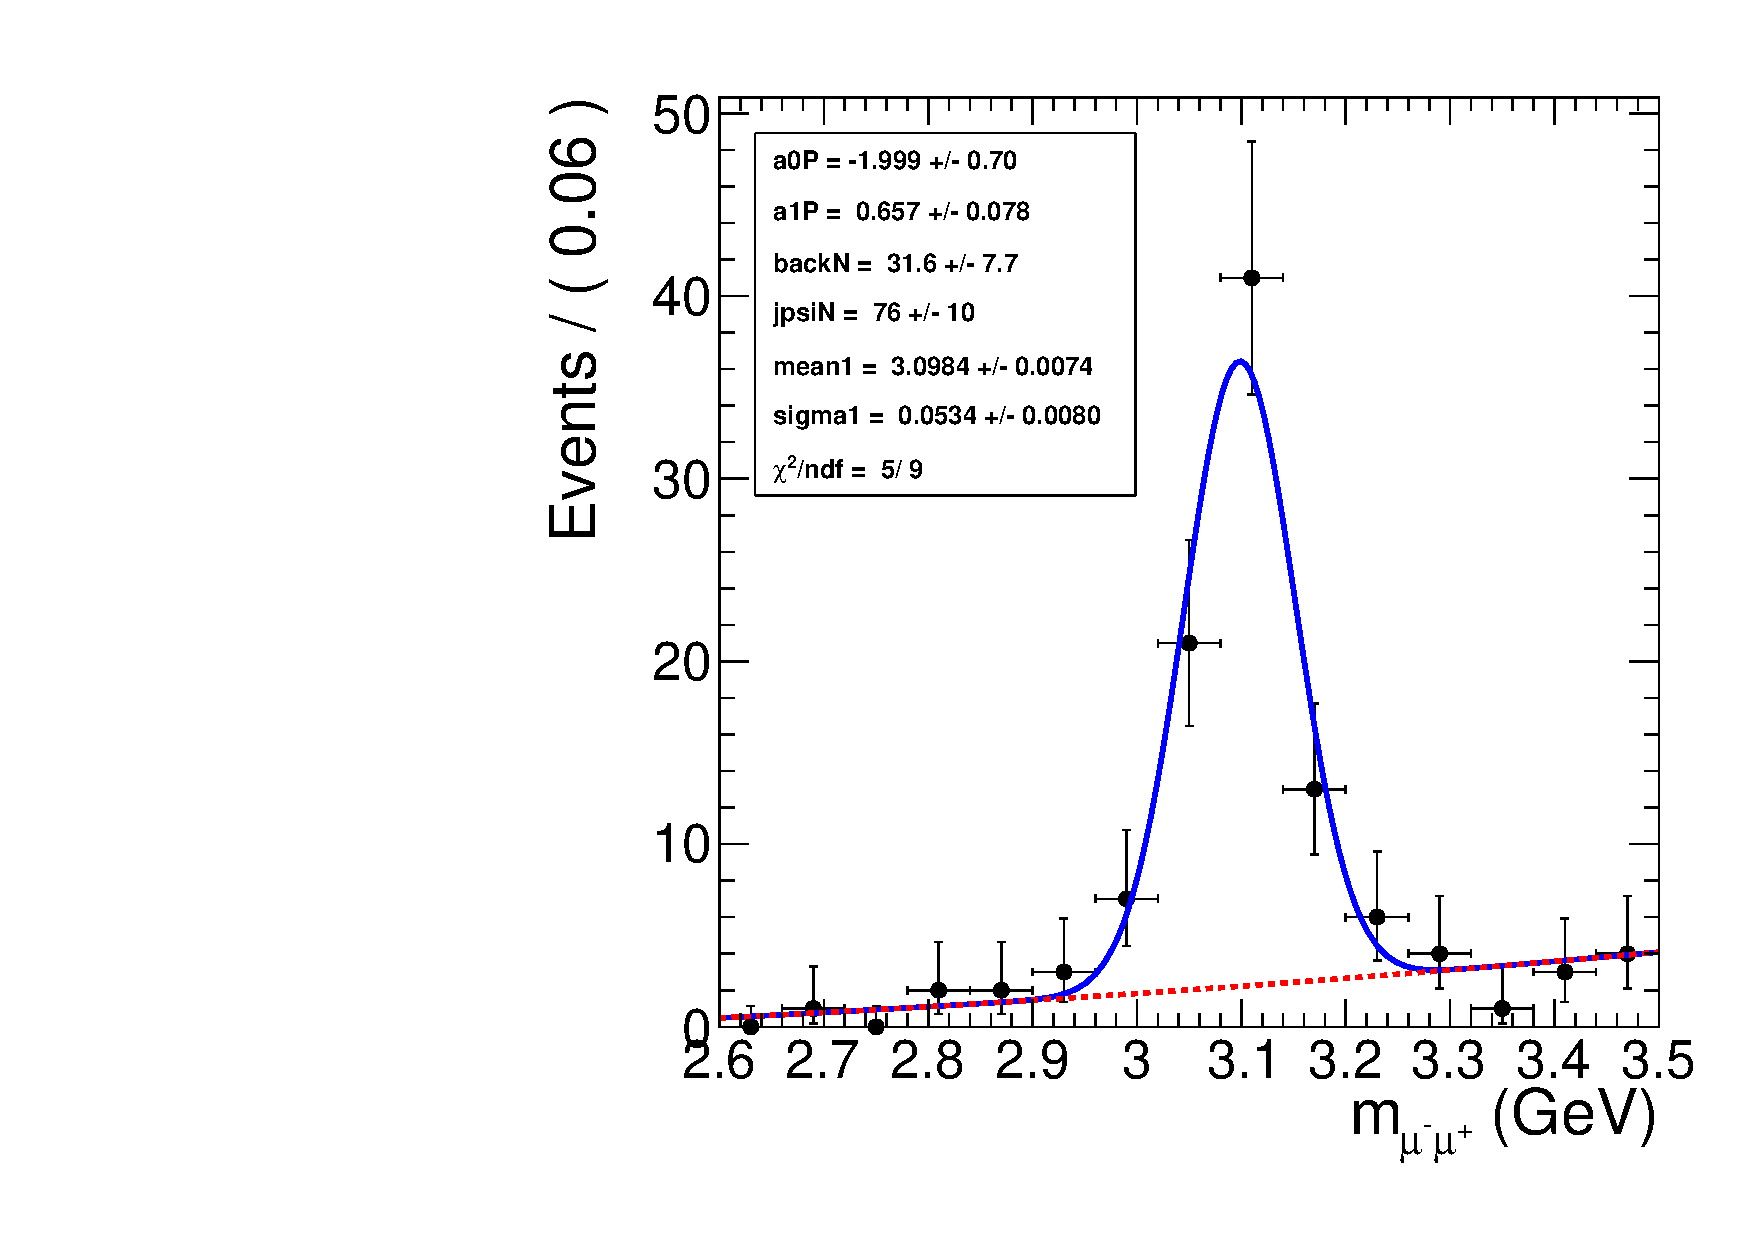
\includegraphics[width=.3\textwidth]{gausLinBkgEst} &
          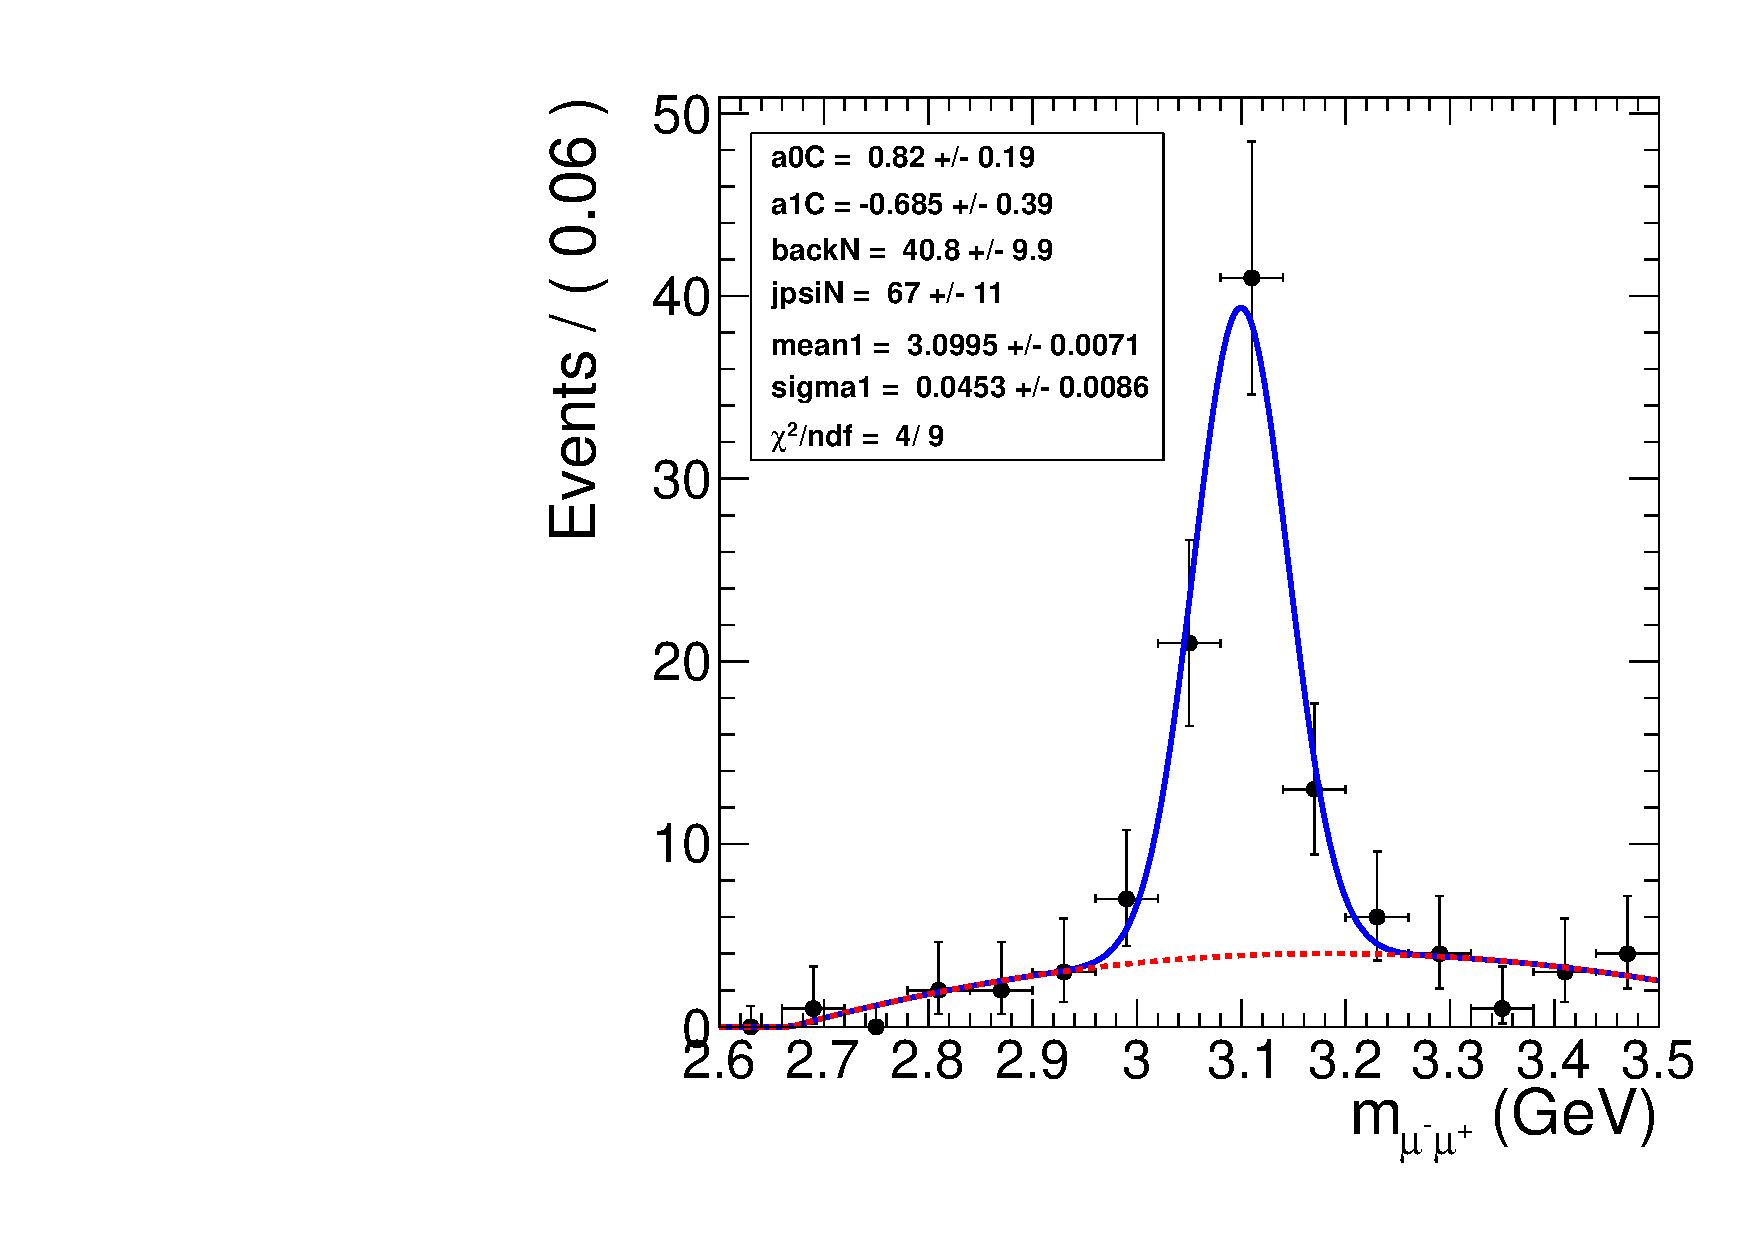
\includegraphics[width=.3\textwidth]{gausCCBkgEst} \\
          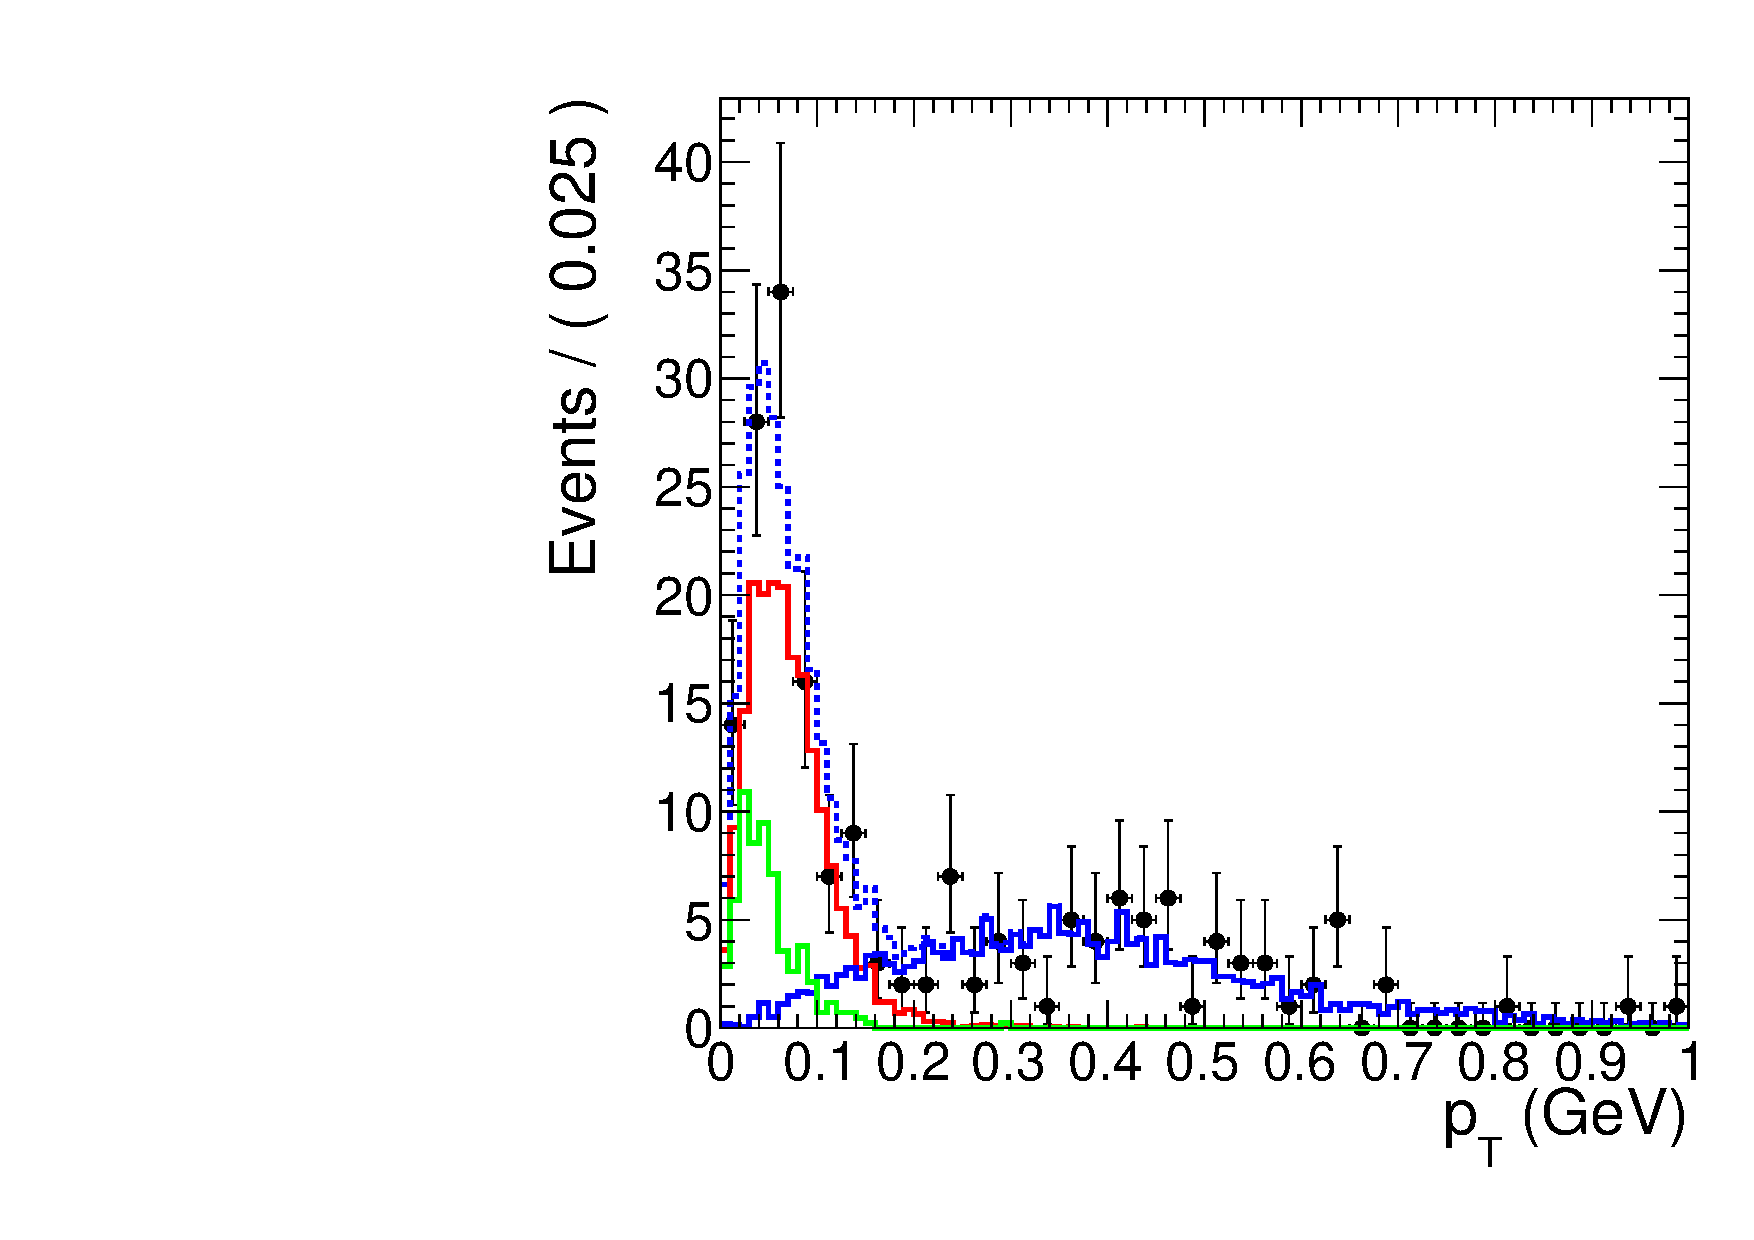
\includegraphics[width=.3\textwidth]{cbPoly} &
          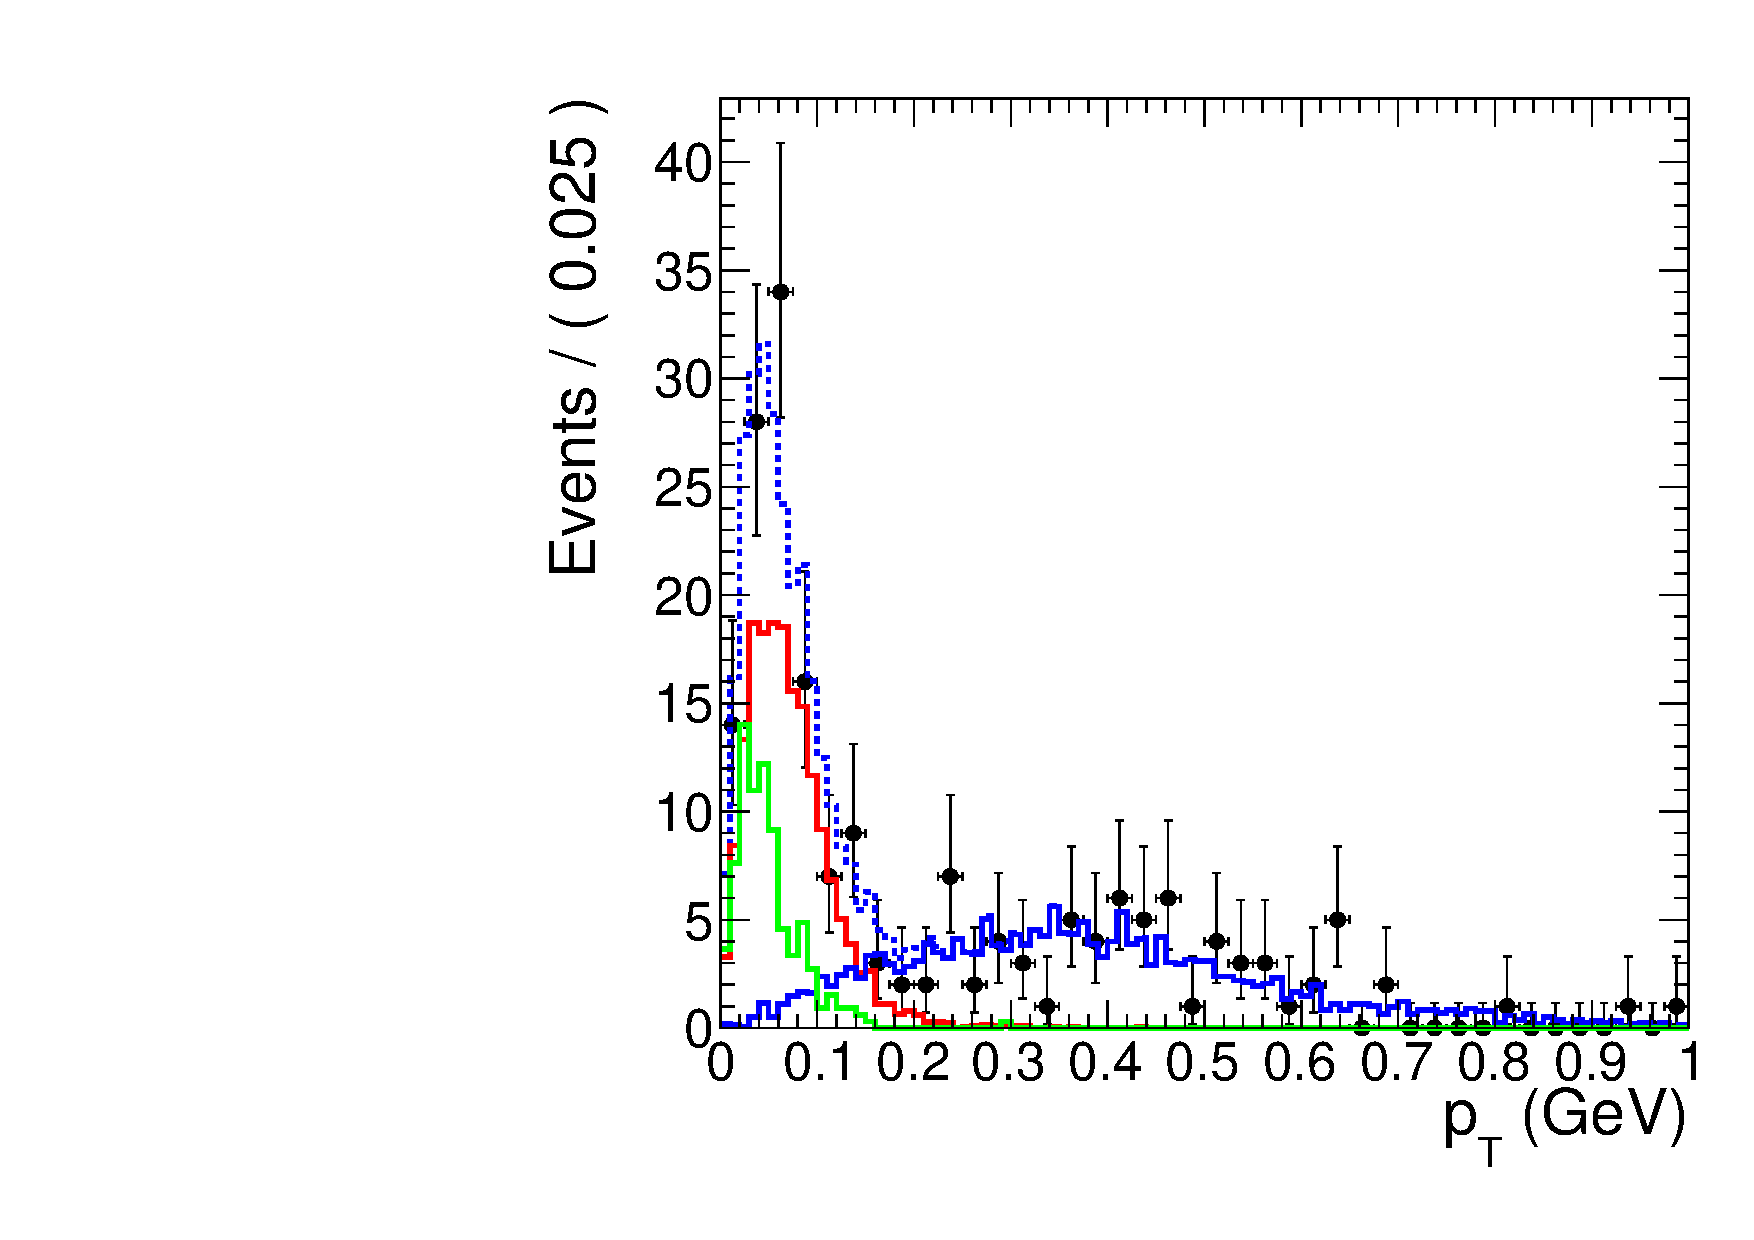
\includegraphics[width=.3\textwidth]{gausLin} &
          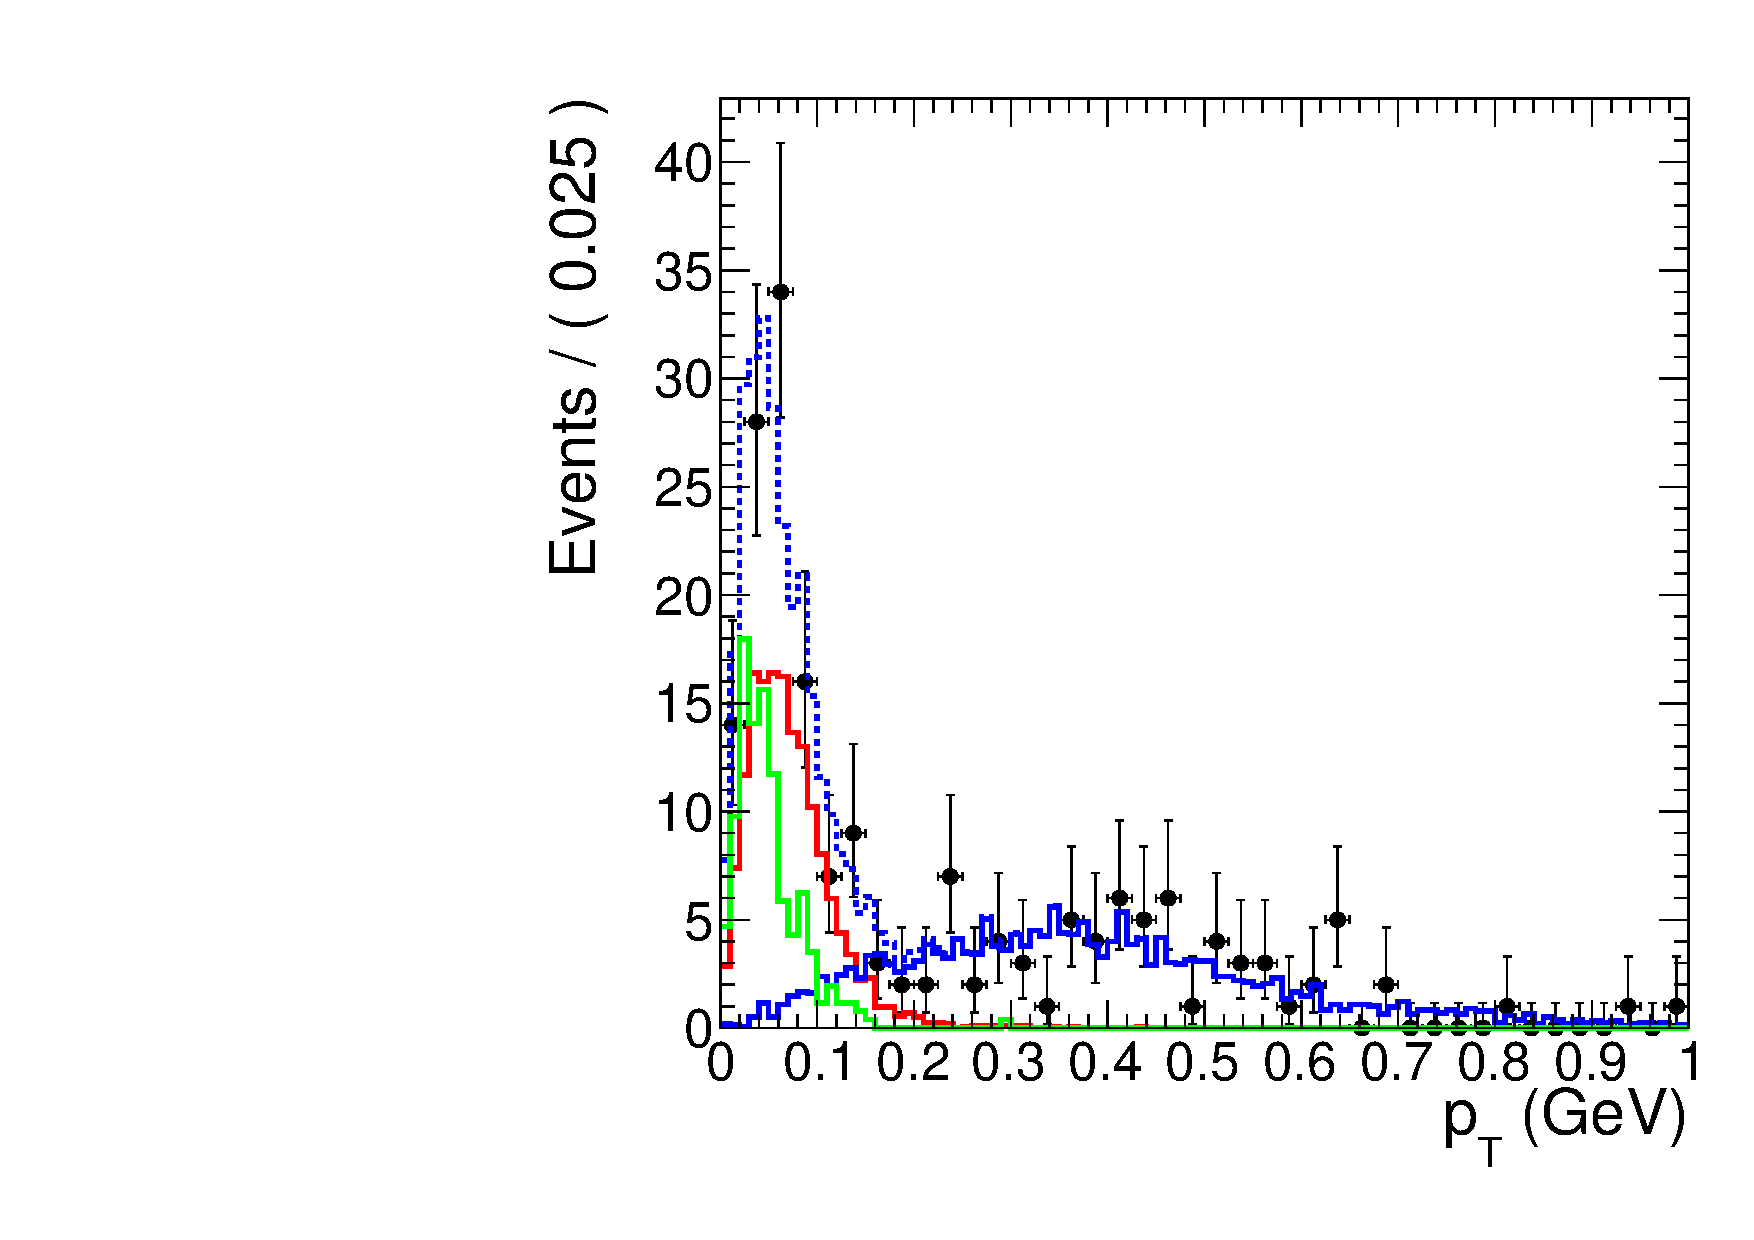
\includegraphics[width=.3\textwidth]{gausCC}
        \end{array} $
        \caption{Various mass distribution fits and the corresponding \pt{}
          template fit.}
        \label{fig:massPtFitsForSyst}
      \end{figure}

      Moving from left to right in Fig~\ref{fig:massPtFitsForSyst}, the 
        contribution from the photon process increases.
      The $\chi^{2}$ pre degree of freedom is similar between the three 
        fits indicating a similar goodness of fit.
      On this basis, neither fit is preferred. 
      The left most fit uses a Crystal Ball function to account for the 
        radiative decay of the final state daughters of the \JPsi{}.
      The low mass exponential portion however picks up background events 
        and overestimates the \JPsi{} contribution. 
      The right most plot fits the background to a 2nd order Cheby-Chev 
        polynomial.
      Because the Cheby-Chev peaks just below the \JPsi{} peak, this fit 
        overestimates the background and in turn underestimates the signal 
        contribution.
      The Gaussian fit with a linear background however does a reasonable job
        of fitting both the background and the signal. 

      From these three fits an upper and lower bound of the systematics due
        the choice of fit functions was estimated. 
      The difference between the Gaussian-Linear fit and the 
        Crystal Ball-polynomial fit was taken as an upper bound. 
      The difference between the Gaussian-Linear fit and the 
          Gaussian-Cheby-Chev fit was taken as a lower bound. 
      The overall systematic uncertainty due to the choose of mass fit 
        functions is found to be +9.5\% -12\%.

    \subsection{Mass fit}

      \begin{figure}[!Hhtb]
        \centering
        $ \begin{array}{cc}
          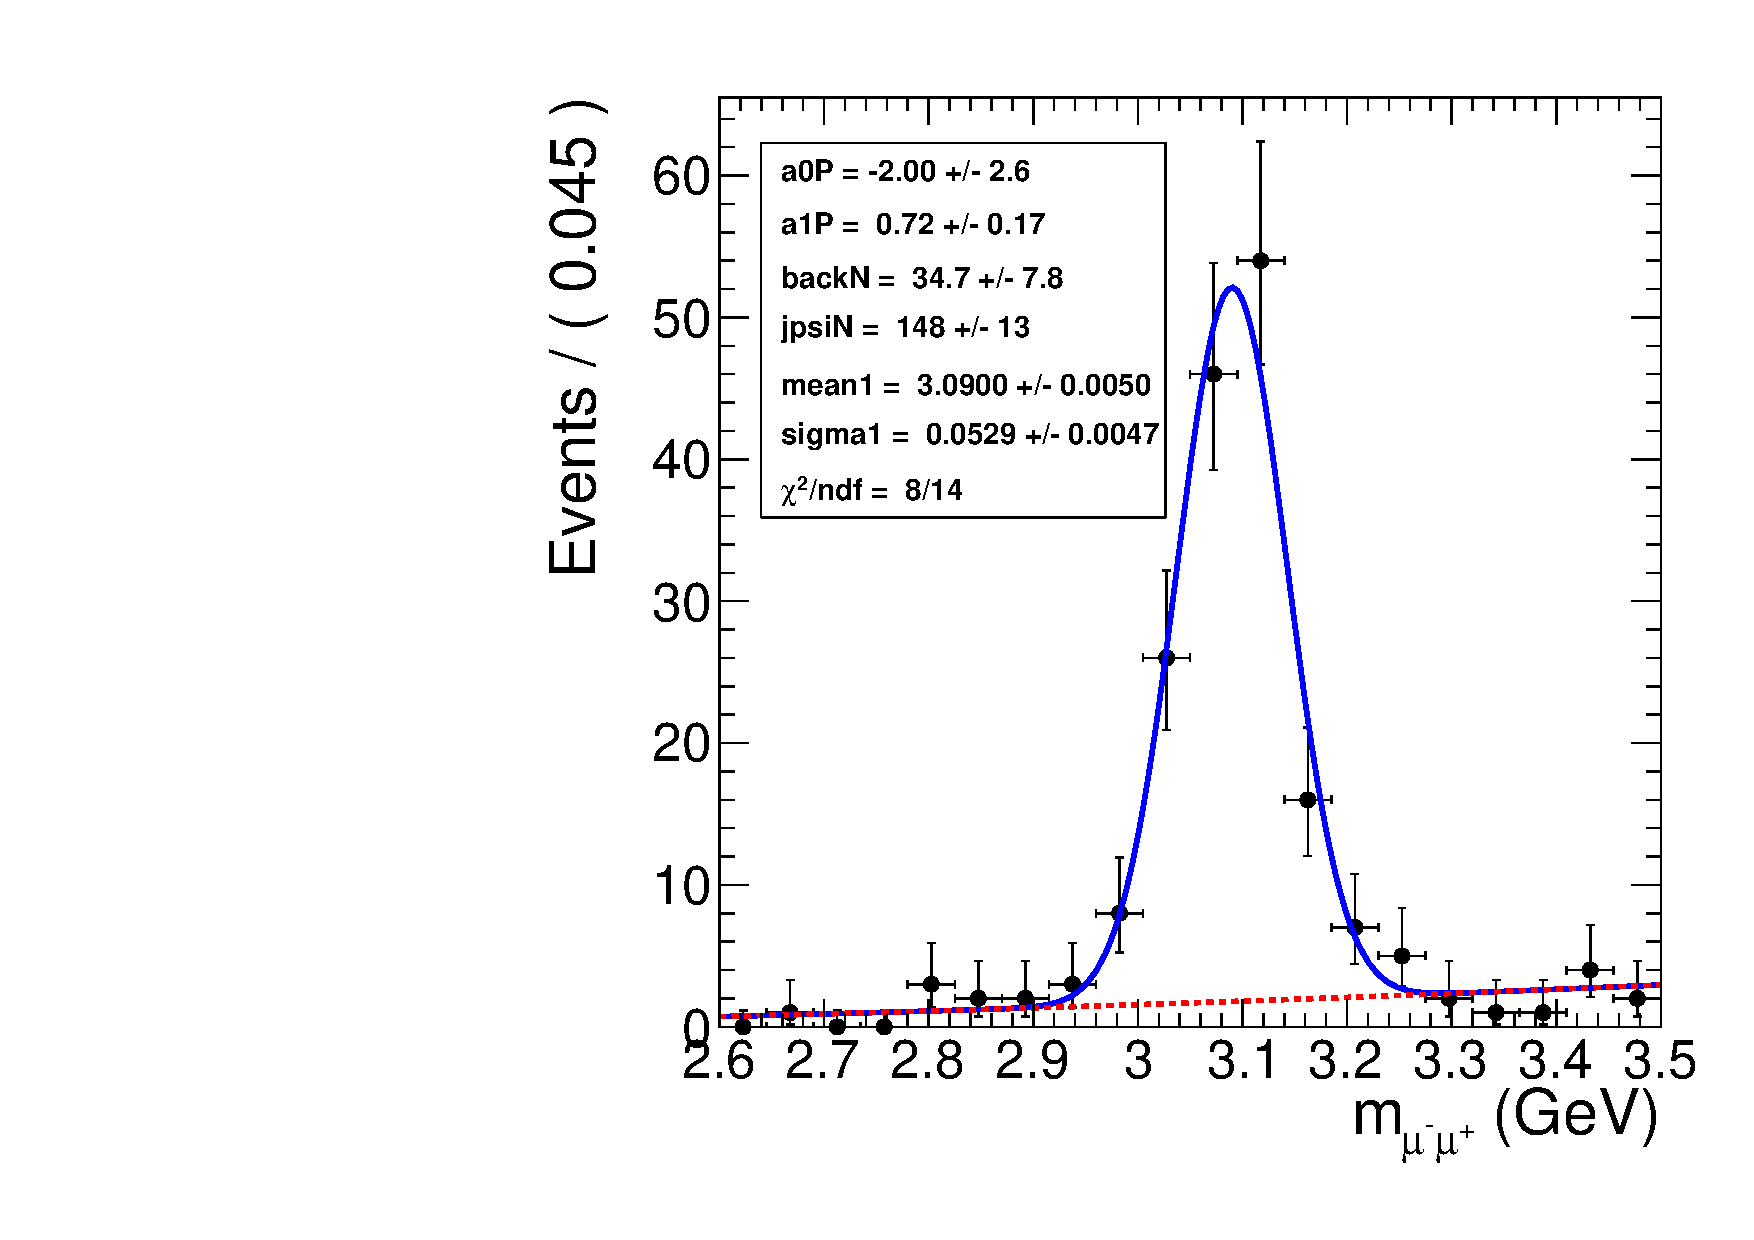
\includegraphics[width=.45\textwidth]{massFitSimple} &
          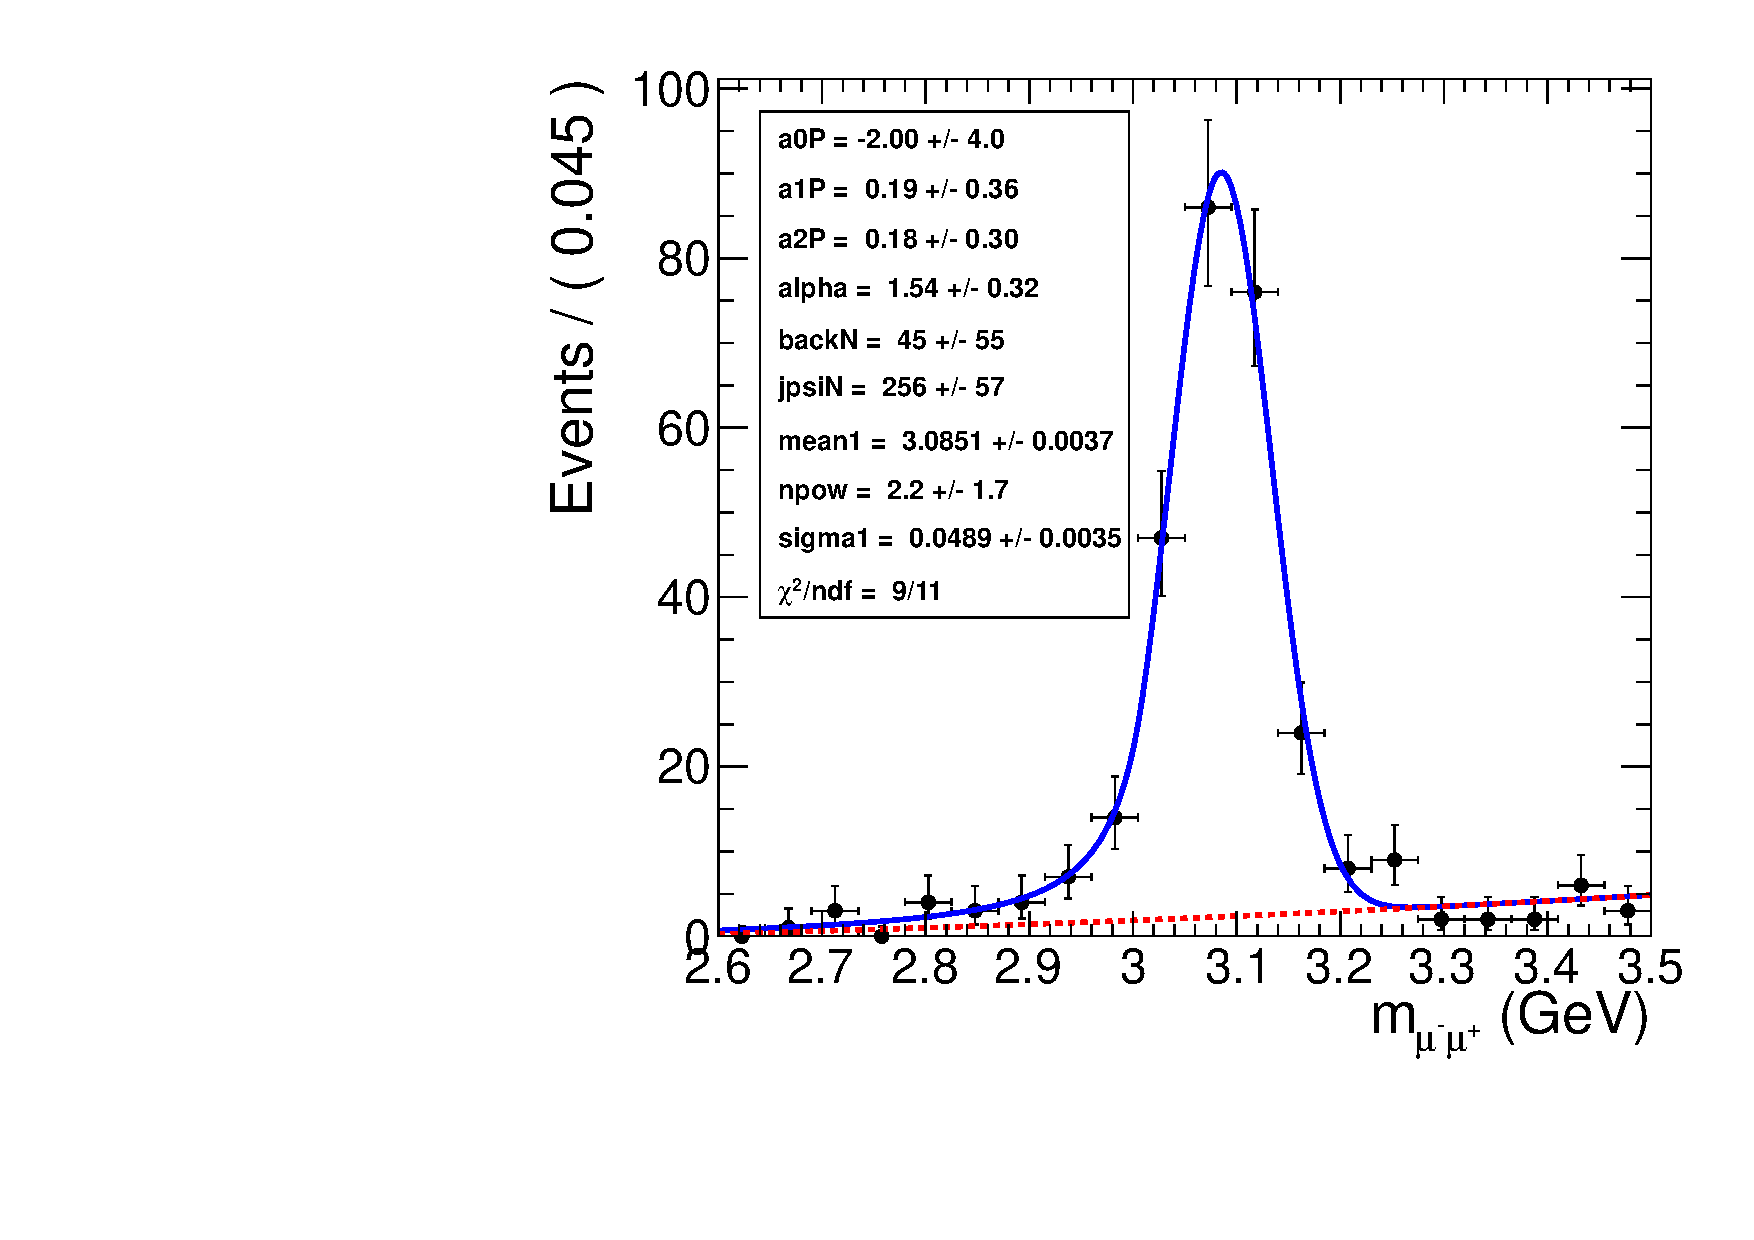
\includegraphics[width=.45\textwidth]{massFitCBPoly2}
        \end{array} $
        \caption{Mass fit to \JPsi{} using Gaussian (Left) and Crystal Ball (Right) for the 
          signal and a polynomial for the background}
        \label{fig:massFitSys}
      \end{figure}
      Fig.~\ref{fig:massFitSys} demonstrates the small dependence the raw 
        \JPsi{} yield has on the fitting function. 
      Both fit functions agree well, with reduced $\chi^{2}$ values below one.
      The Crystal ball fit give an upper estimate for the \JPsi{} yield.
      The Gaussian fit gives an lower estimate. 
      The main difference comes from the lower mass tails.
      In the Crystal ball fit the lower tail is considered to be signal due to 
        shifting of the mass spectrum to lower mass due to radiation from the 
        final state muons. 
      In the Gaussian fit the lower mass tail is considered to be background and 
        the signal is sharper.

      As check on the simultaneous \pt{} and mass fit, the mass fit is done
        using mass templates from STARlight.
      \begin{figure}[!Hhbt]
        \centering
        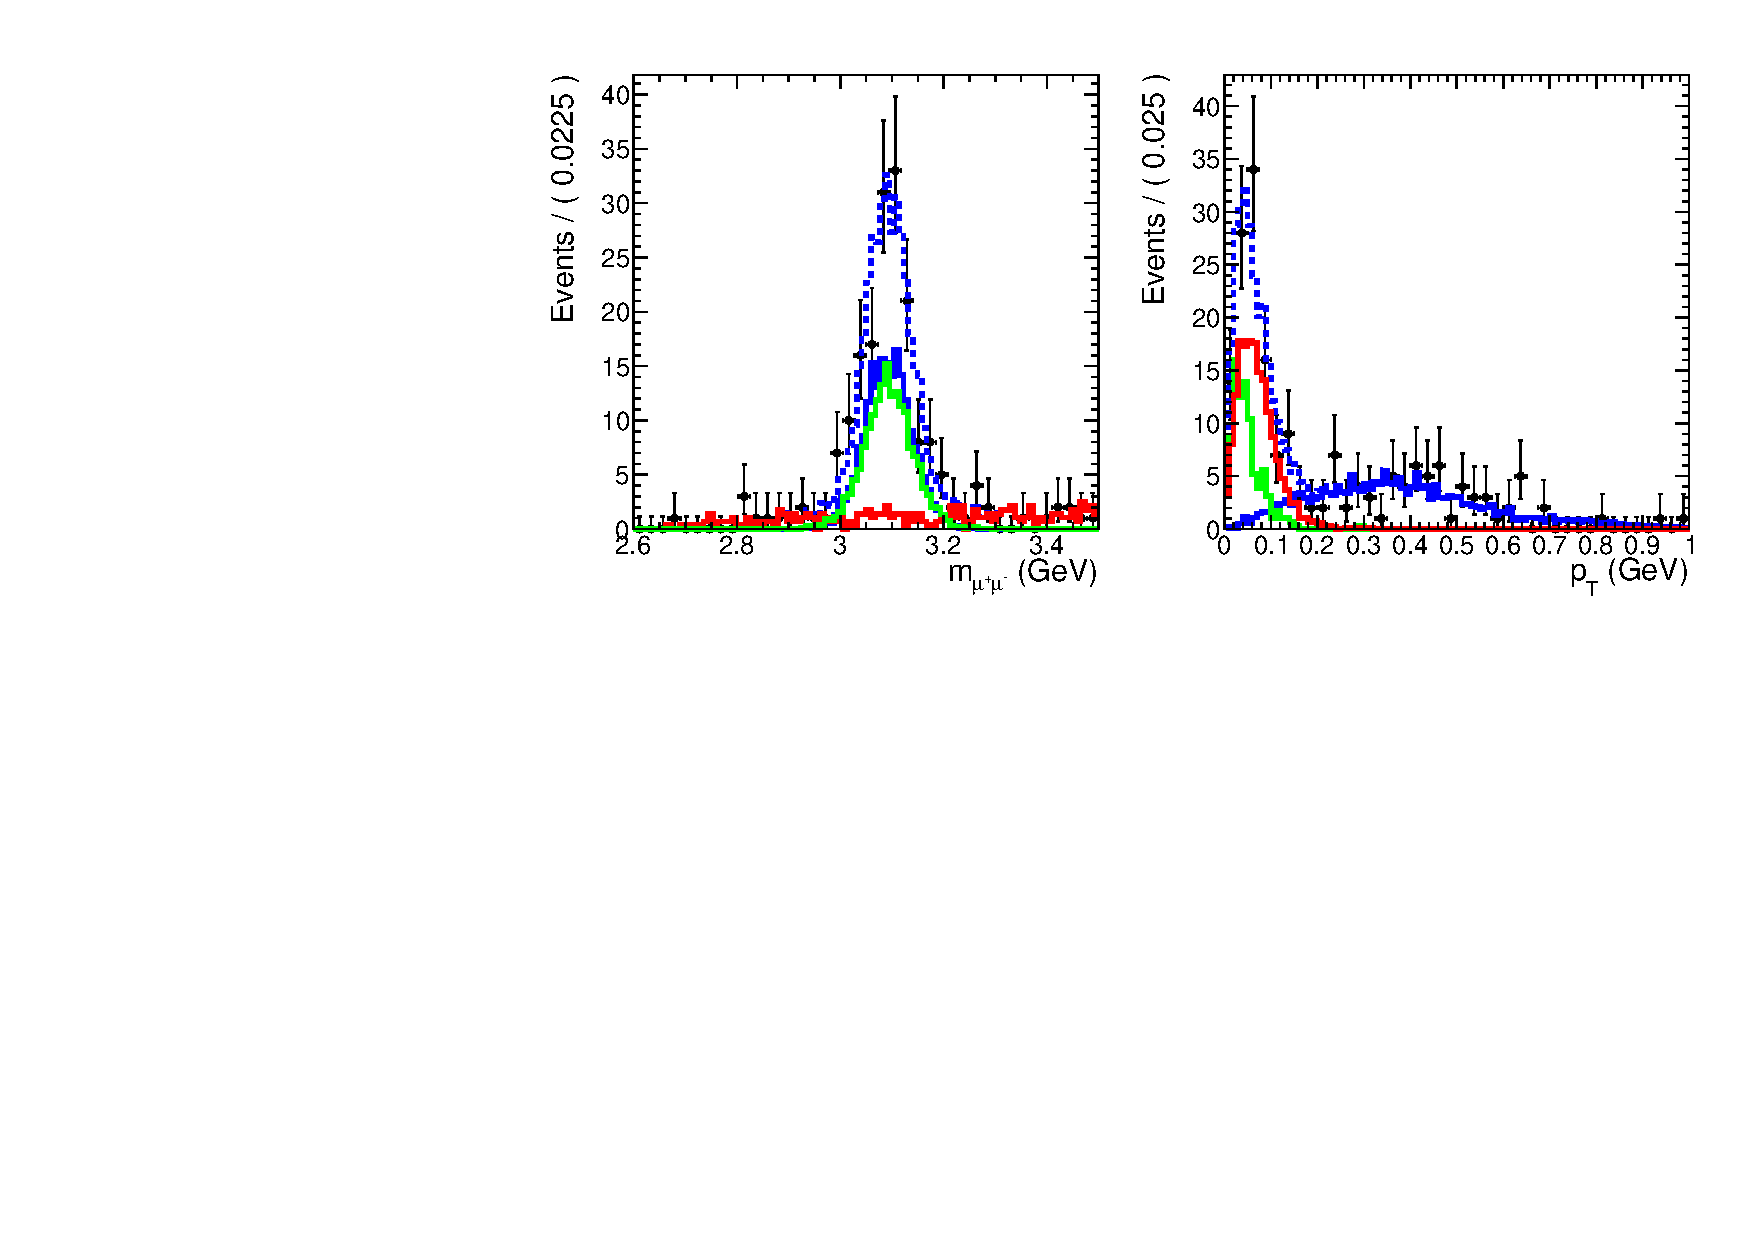
\includegraphics[width=0.6\textwidth]{ptMassSimTemp}
        \caption{Simultaneous fit to the mass and \pt{} using mass templates
          for the mass fit. }
        \label{fig:simFitTemp}
      \end{figure}

    \subsection{MC acceptance}
      The MC derived acceptance correction factors depend on the input physics
        generator. 
      The underlaying \pt{} distribution was assumed to be correctly 
        described by STARlight for the coherent cross section measurement.
      To estimate the effect of changing the underlaying \pt{} distribution 
        on the acceptance measured from the MC, the incoherent sample was used 
        to correct the coherent yield.
      By using the broader \pt{} distribution of the incoherent process, an 
        estimate of acceptance measurements dependence on the assumed shape of
        the \pt{} distribution was obtained.
      The systematic uncertainty due to the dependence of the acceptance 
        correction on the \pt{} distribution of the input physics generator
        was estimated by the difference between the correction factors from 
        the coherent and incoherent MC samples. 
      Half the difference was used as the estimate and was found to be 1.1\%.

      \begin{figure}[!Hhbt]
        \centering
        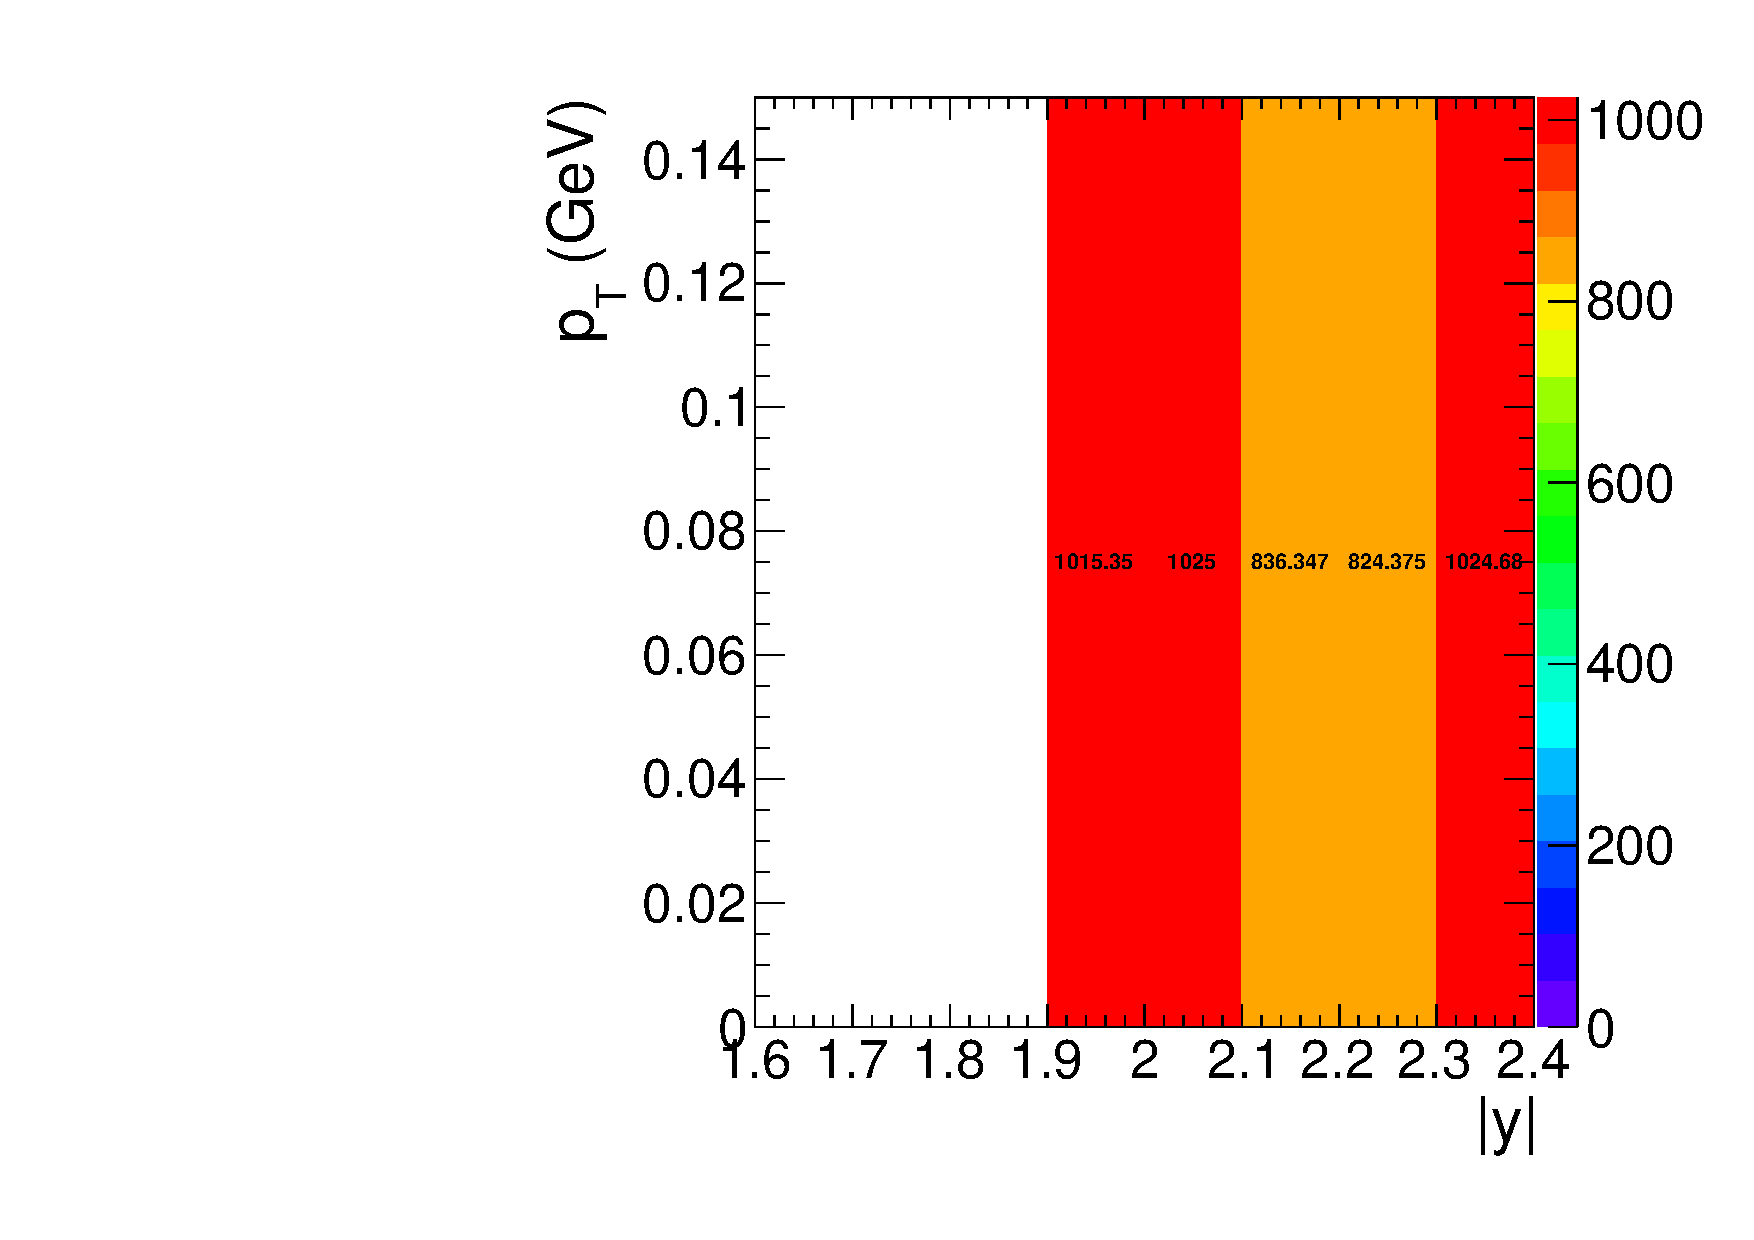
\includegraphics[width=0.6\textwidth]{coCorInCoAcc}
        \caption{Yields corrected by the MC incoherent acceptance map.}
        \label{fig:coYieldInCoCor}
      \end{figure}

      The effect of polarization was estimated by correcting by the acceptance
        for an unpolarized \JPsi{} sample.
      \begin{figure}[!Hhtb]
        \centering
        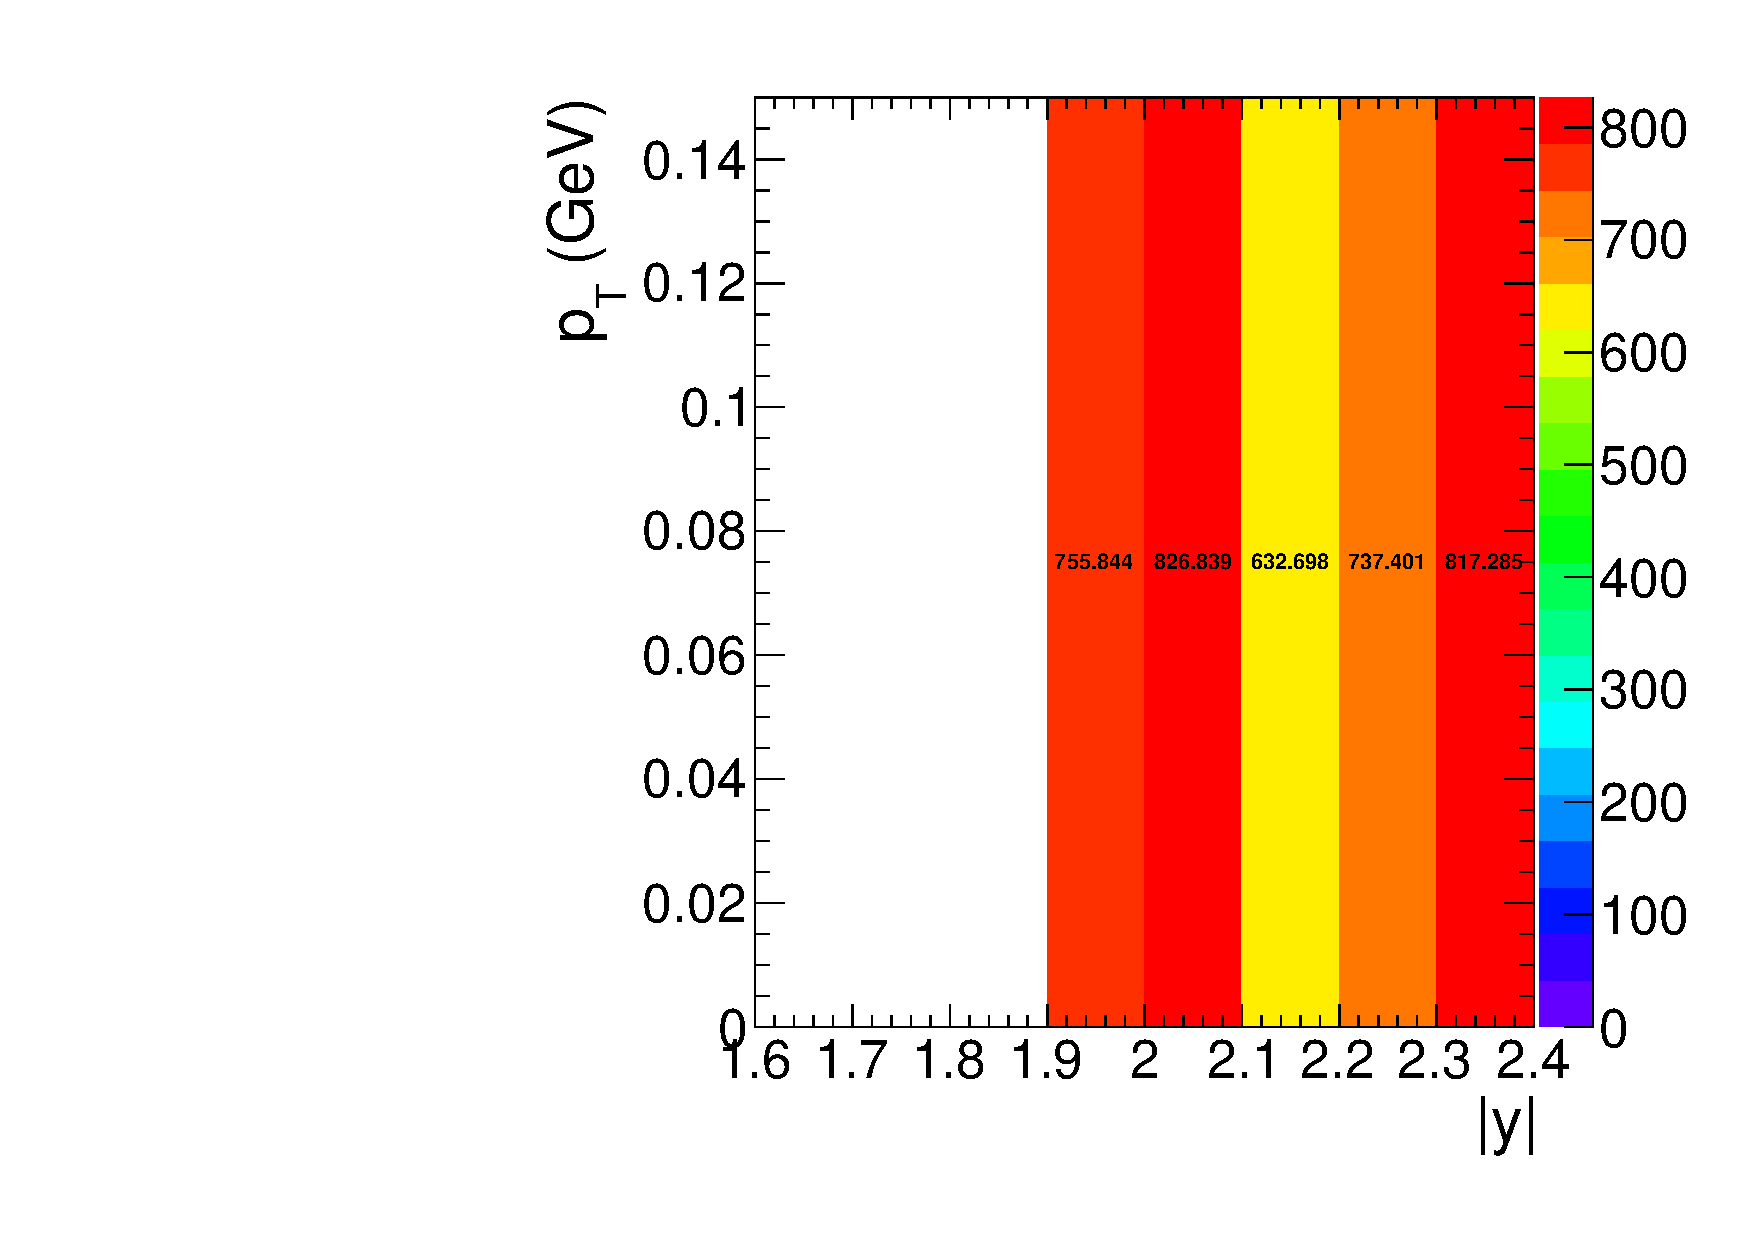
\includegraphics[width=0.6\textwidth]{coCoGaussGun}
        \caption{Yields corrected by an unpolarized \JPsi{} sample.}
        \label{fig:coYieldGaussCor}
      \end{figure}

    \subsection{ZDC reconstruction}
      An additional method for estimating the ZDC neutron thresholds was used
        to estimate the systematic errors on the threshold measurements.  
      This additional method, used in previous ZDC measurements, differs 
        in the way the signal time slices are used to calculate the signal from
        each channel.
      In the standard method, the signal is taken from the sum of time slices 
        4, 5, and 6.
      To estimate the event by event noise pedestal the sum of time slice 
        1 and 2 are used. 
      The signal for an individual ZDC channel is then calculated as the 
        sum of the signal time slices minus the sum of the noise time slices
        weighted by a factor of 3/2 to account for the differing number of 
        noise versus signal time slices.
      The advantage of the standard method is that by using multiple signal
        and noise time slices the signal and noise are effectively averaged
        reducing time slice to time slice fluctuations.
      However, by using time slices 1 and 2 for measuring the noise, the noise
        can only be measured half the time due to unmeasurable negative 
        fluctuations of the dominant low frequency component of the noise.

      As in the new method described in Section~\ref{sec:breakUpDet}, 
        the standard method combines the channels to create a signal 
        measurement from the whole of each side of the ZDC, one
        measurement for ZDC$^{+}$, and one for ZDC$^{-}$.
      The noise subtracted signal from each of the HAD channels are added 
        together.
      Then the EM section channels are summed. 
      The EM section is weighted by a factor of 0.1 as in the new method. 
      After the weighting the EM and HAD channels are added to each to create
        one measurement for ZDC$^{+}$ and another measurement for ZDC$^{-}$.

      Fig.~\ref{fig:zdcM1Fit} shows the spectra for ZDC$^{+}$ and ZDC${-}$ 
        using the standard method. 
      The same fit used for the new method is applied to standard method. 
      As in the new method, the single neutron threshold is set to 2$\sigma$
        below the mean from the fit to the one neutron peak.
      The multi-neutron threshold was set to 2$\sigma$ above the one neutron
        peak.

      \begin{figure}[!Hhtb]
        \centering
        $ \begin{array}{cc}
          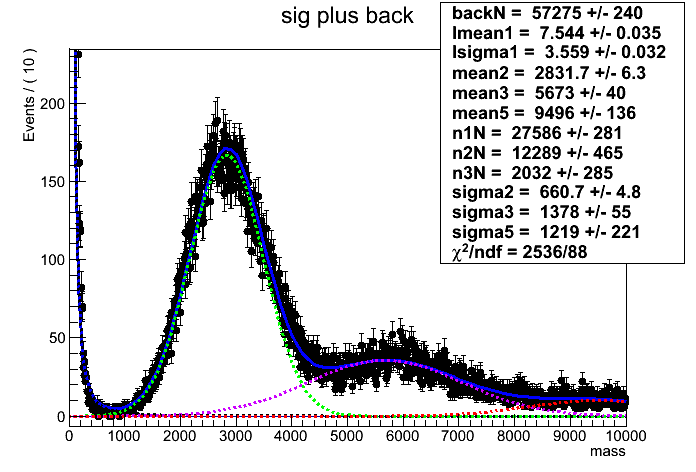
\includegraphics[width=0.45\textwidth]{zdcMinusZBFitTimeCut} &
          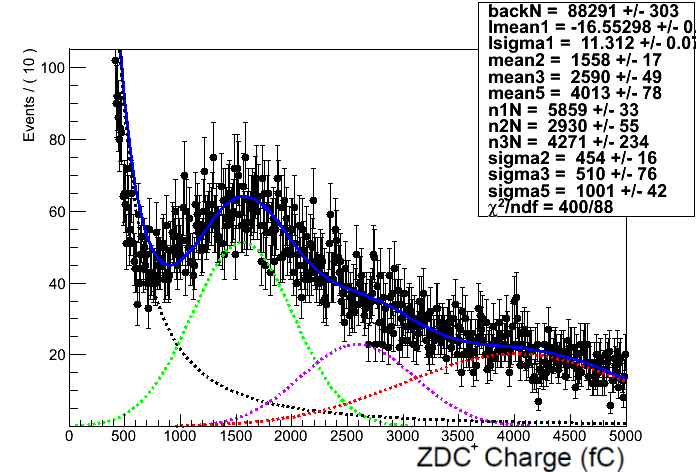
\includegraphics[width=0.45\textwidth]{zdcPlusZBFitTimeCut}
        \end{array} $
        \caption{Fit to charge spectrum from ZDC$^{-}$ (left) and ZDC$^{+}$ 
          (right) using the standard reconstruction method}
        \label{fig:zdcM1Fit}
      \end{figure}

      The systematic uncertainty due to the ZDC reconstruction method are
        estimated from the difference between the UPC \JPsi{} candidate yields.
      Both the reconstruction method and thresholds were changed to calculate 
        the effect of the reconstruction method.
      The yields for the new and standard ZDC reconstruction method in the Xn0n
        break up were found to be 298 and 315 respectively. 
      Half the difference between the two methods was used as an estimated of 
        the systematic uncertainty.
      The systematic uncertainty due to the ZDC reconstruction method was 
        found to be 2.9\%.

    \subsection{ZDC trigger efficiency}
      The ZDC trigger efficiency measurement is sensitive to the underlying 
        neutron distribution.
      The more neutrons that hit the ZDC, the higher the trigger efficiency 
        will be.
      To estimate the effect the input sample has on the efficiency, the ZDC 
        trigger efficiency was measured from five different samples.
      The Table~\ref{tab:zdcEfficiencySys} shows the results from the 
       three samples, which require reconstruction a pixel track to reduce
       the contribution from noise. 
      Both the new and standard ZDC reconstruction methods are shown for 
        comparison.
      \begin{table}
        \centering
        \begin{tabular}{|c|c|c|c|c|}
          \hline ZDC Side & Reco Method & N$_{events}$ & N$_{trig}$ & $\varepsilon_{ZDC}$ \\ \hline
           \multicolumn{5}{|c|}{(ZDC$^{+}$ or ZDC$^{-}$) and 1 pixel track} \\ \hline 
           ZDC$^{-}$ & standard & 72946  & 71688 & 0.982 $\pm$ 0.005 \\ \hline
           ZDC$^{-}$ & new & 73028  & 71706  & 0.982  $\pm$ 0.005  \\ \hline
           ZDC$^{+}$ & standard & 76137  & 71786  & 0.943  $\pm$ 0.005  \\ \hline
           ZDC$^{+}$ & new & 76132  & 71859  & 0.944  $\pm$ 0.005  \\ \hline
           \multicolumn{5}{|c|}{(ZDC$^{-}$ or ZDC$^{+}$), 1 pixel track, and L1 EG trigger } \\ \hline 
           ZDC$^{-}$ & standard & 613758  & 602123  & 0.9810 $\pm$ 0.0018 \\ \hline
           ZDC$^{-}$ & new & 614014  & 601863  & 0.9802 $\pm$ 0.0018 \\ \hline
           ZDC$^{+}$ & standard & 643905  & 602671  & 0.9360  $\pm$ 0.0017 \\ \hline
           ZDC$^{+}$ & new & 647888  & 603089  & 0.9309  $\pm$ 0.0017 \\ \hline
           \multicolumn{5}{|c|}{(ZDC$^{-}$ or ZDC$^{+}$), 1 pixel track, and L1 Muon trigger} \\ \hline 
           ZDC$^{-}$ & standard & 65466  & 63376  & 0.968 $\pm$ 0.005  \\ \hline
           ZDC$^{-}$ & new & 65543  & 63358  & 0.967 $\pm$ 0.005 \\ \hline
           ZDC$^{+}$ & standard & 71929  & 63512  & 0.883  $\pm$ 0.005 \\ \hline
           ZDC$^{+}$ & new & 72932  & 63582  & 0.872  $\pm$ 0.005 \\ \hline
         \end{tabular}
        \caption{ZDC trigger efficiencies for ZDC reconstruction method 1 and 
          2 for trigger sample which require a pixel track.}
        \label{tab:zdcEfficiencySys}
      \end{table}

      The amount of electronic noise in the sample also effects the measurement.
      The more noise sits below the one neutron peak, the lower the efficiency 
        is. 
      In Table~\ref{tab:zdcEfficiencySysNoiseSample}, the Zero Bias sample 
        compared the Zero Bias sample with the timing cuts, which were 
        described in the previous section, shows a significant increase in 
        the estimated efficiency in the sample with reduced noise. 
      The same increase is seen when comparing the ZDC triggered sample with 
        the ZDC triggered sample that also requires a pixel track. 
      The effect of the electronic noise is also present in the difference seen
        in using the two methods.
      As seen in Fig.~\ref{fig:zdcSpec2v1}, the new reconstruction method 
        shows better separation of the one neutron peak from the electronic 
        noise, in particular in ZDC$^{+}$ where the signal gain is lower.
      For this reason, the Zero Bias data, which contains the largest 
        contribution from electronic noise, shows the most separation between 
        the two methods and give the lowest estimate for the ZDC trigger 
        efficiency.
      \begin{table}
        \centering
        \begin{tabular}{|c|c|c|c|c|}
          \hline ZDC Side & Reco Method & N$_{events}$ & N$_{trig}$ & $\varepsilon_{ZDC}$ \\ \hline
          \multicolumn{5}{|c|}{ Zero Bias with ZDC timing cuts} \\ \hline 
           ZDC$^{-}$ & standard & 88676  & 84429  & 0.9521 $\pm$ 0.0046 \\ \hline
           ZDC$^{-}$ & new & 88480  & 84202  & 0.9517 $\pm$ 0.0046 \\ \hline
           ZDC$^{+}$ & standard & 59878  & 54728  & 0.9140  $\pm$ 0.0054 \\ \hline
           ZDC$^{+}$ & new & 60467  & 54733  & 0.9052  $\pm$ 0.0053 \\ \hline
           \multicolumn{5}{|c|}{(ZDC$^{-}$ or ZDC$^{+}$)} \\ \hline 
           ZDC$^{-}$ & standard & 30986 & 30333 & 0.9789 $\pm$ 0.0079 \\ \hline
           ZDC$^{-}$ & new & 31029 & 30339 & 0.9778 $\pm$ 0.0079 \\ \hline
           ZDC$^{+}$ & standard & 39178 & 30164 & 0.7699 $\pm$ 0.0059 \\ \hline
           ZDC$^{+}$ & new & 35703 & 30443 & 0.8527 $\pm$ 0.0067 \\ \hline
           \multicolumn{5}{|c|}{ Zero Bias} \\ \hline 
           ZDC$^{-}$ & standard & 109967  & 101598  & 0.9239 $\pm$ 0.0040 \\ \hline
           ZDC$^{-}$ & new & 110230  & 101561  & 0.9214 $\pm$ 0.0040 \\ \hline
           ZDC$^{+}$ & standard & 253241  & 86660  & 0.3422 $\pm$ 0.0013 \\ \hline
           ZDC$^{+}$ & new & 156336  & 87401  & 0.5591 $\pm$ 0.0024 \\ \hline
         \end{tabular}
        \caption{ZDC trigger efficiencies for ZDC reconstruction method 1 and 
          2 for samples that do not require a pixel track.}
        \label{tab:zdcEfficiencySysNoiseSample}
      \end{table}

      The systematic uncertainty in the ZDC trigger efficiency due to the 
        uncertainty in the underlying distribution was estimated by calculating 
        the standard deviation of efficiency measurements in Table~\ref{tab:zdcEfficiencySys}.
      The uncertainty in the ZDC trigger efficiency is taken to be \DIFaddbegin \DIFadd{1\% for 
      ZDC$^{-}$ and 4\% for ZDC$^{+}$.
}\DIFaddend 

    \subsection{ZDC reconstruction method comparison}
      The new method relative to the standard method separates low signal from 
        the noise more effectively for both sides of the ZDC.
      This is particularly important for ZDC$^{+}$ where the 1st HAD section
        had a lower gain than the other sections. 
      The ZDC$^{+}$ and ZDC$^{-}$ signals near the one neutron peak using the
        standard and new reconstruction methods were plotted for comparison in 
        Fig.~\ref{fig:zdcSpec2v1}.
      \begin{figure}[h]
        \centering
        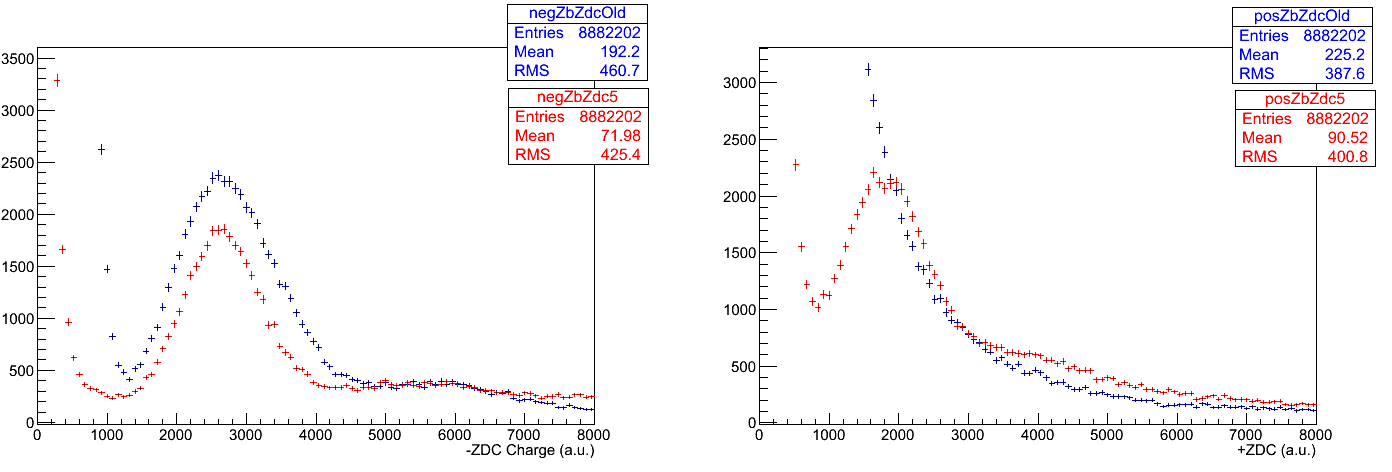
\includegraphics[width=\textwidth]{zdcSpec2v1}
        \caption{Comparison of the \textcolor{red}{new} ZDC reconstruction 
          method and the \textcolor{blue}{standard} method for ZDC$^{-}$ (left) and 
          ZDC$^{+}$ (right).}
        \label{fig:zdcSpec2v1}
      \end{figure}
      In Fig.~\ref{fig:zdcSpec2v1}, the shrinking of width of the noise peak 
        around zero in the new method versus the old method is apparent for
        both ZDC$^{+}$ and ZDC$^{-}$.
      For the standard method no single neutron peak is resolved in ZDC$^{+}$,
        whereas the single neutron peak is resolved using the new method. 

      Timing cuts were applied to enhance the signal relative to the background
        in order to resolve the one neutron peak in ZDC$^{+}$ using the 
        standard method. 
      Because the products of the collision are synced with time slice 4, noise
        can be rejected by selecting channels where the maximum signal falls 
        into time slice 4.
      The noise will have no preferred time slice (see Fig.~\ref{fig:zdcPulseShape}). 
      Using this fact, signal can be preferably selected by requiring that the
        hadronic channels of the ZDC have a peak signal in the fourth time 
        slice.
      Through these timing cuts the single neutron peak was recovered using the
       standard reconstruction for ZDC$^{+}$.

      To examine the effectiveness of the timing cuts, event by event noise 
        subtraction was removed from the standard reconstruction.
      The signal from each channel was taken from time slices 4,5, and 6 with
        out subtracting 1 and 2.
      The signal spectrum from ZDC$^{-}$ was then plotted with the result
        shown in Fig.~\ref{fig:zdcTimingCuts}.
      \begin{figure}[!Hhbt]
        \centering
        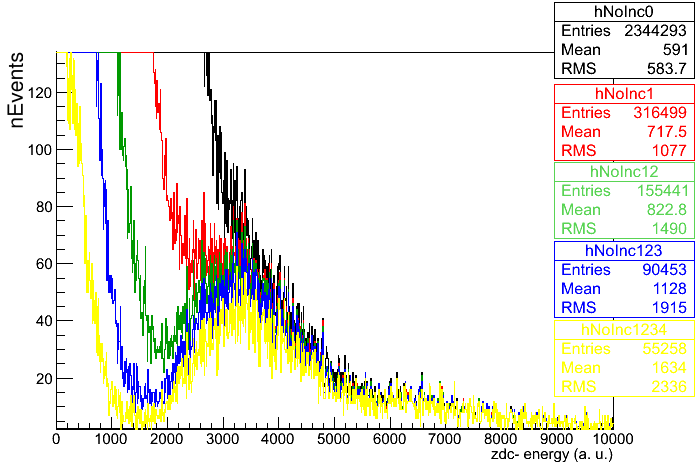
\includegraphics[width=0.6\textwidth]{zdcMinusSingleNuNoInc}
        \caption{Effects of requiring in-time signal in successively more 
          ZDC hadronic channels, no timing, at least \textcolor{red}{one}, at least \textcolor{green}{two},
            at least \textcolor{blue}{three}, and all \textcolor{yellow}{four} HAD channels have a maximum signal
            in the fourth time slice.}
        \label{fig:zdcTimingCuts}
      \end{figure}
      As each additional hadronic channel is required to have a maximum signal
        in the fourth time slice, the single neutron peak emerges. 
      Fig.~\ref{fig:zdcTimingCuts} demonstrates that the single neutron peak 
        can be recovered from the noise using timing cuts alone. 

      Using the standard noise subtraction method, the same signal that emerges
        from the timing cuts alone appear without timing cuts.
       \begin{figure}[h]
        \centering
        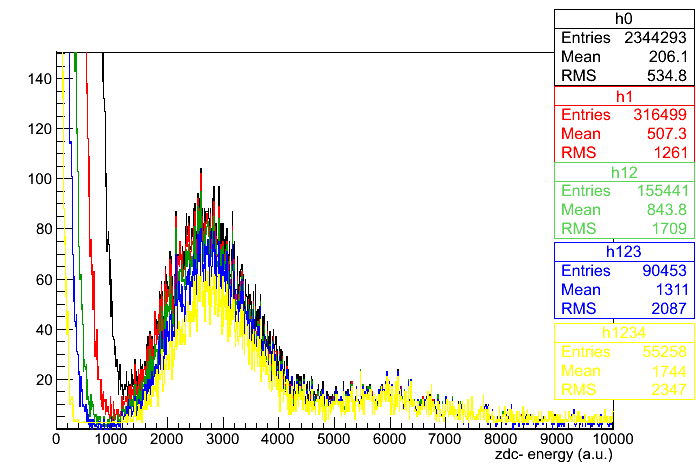
\includegraphics[width=0.6\textwidth]{zdcMinusSingleNuNoSub}
        \caption{Effect of ZDC signal timing requirements after noise 
          subtraction.}
        \label{fig:zdcTimingAfterNoiseSub}
      \end{figure}
      Fig.~\ref{fig:zdcTimingAfterNoiseSub} confirms that both noise 
        subtraction and the timing requirement produce the same signal.
      This gives confidence that the signal is not an artifact of either cut, 
        but the true neutron signal.

       Fig.~\ref{fig:zdcTimingAfterNoiseSub} and Fig.~\ref{fig:zdcSpec2v1} 
        demonstrate the consistence of the using timing cuts and noise 
        subtraction to enhance the signal neutron peak. 
      Fig.~\ref{fig:zdcTimingAfterNoiseSub} confirms the legitimacy of the 
        timing requirement method in ZDC$^{-}$ by showing the that the same
        signal emerges from the noise subtraction method as the timing method.
      Fig.~\ref{fig:zdcSpec2v1} demonstrates the corresponds between
        the new noise subtraction method and the standard method on in 
        ZDC$^{-}$ where signal is better separated from the electronic noise. 
      This allows for confidence that the signal seen in ZDC$^{+}$ using 
        the new method is the one neutron peak.

    \subsection{Tag and probe}
      The main purpose for fitting the mass spectra to estimate the efficiency
        is to separate the background from true signal. 
      The background may not have the same efficiency as the signal, so 
        separating the two is important if this is the case.
      In the tag and probe fit the signal peak from the \JPsi{} resonance
        is fit to the probes, passing probes, and failing probes alike (see
        Fig.~\ref{fig:tnpFitPlot}). 
      The signal shape, if from the same physical signal, will be 
        identical in each of the three distributions. 
      The background is for the passing and failing probes is fit using 
        different parameters for the background because the background
        may come from different physical processes than the signal or 
        non-physical sources like combinatorial backgrounds or misidentified
        fake particles.
      When the background comes from sources other than the physical signal,
        the background may give an efficiency estimate that is lower than
        the signal. 

      The trigger efficiency measured by the tag and probe method depend on
        the fitting functions use to estimate the background and signal 
        contributions. 
      Depending on what functions is used to fit the spectra, the amount of
        amount of background can be over or underestimated and effect the 
        efficiency measurement.
      To estimate this effect, the tag and probe efficiencies were additionally
        measured by counting probes in the \JPsi{} mass window. 
      The whole mass window is used to estimate the efficiency including all 
        the events from the mass side bands.
      In this way, a worst case scenario estimate is given where all background
        events are included as signal. 
      \begin{figure}[!Hhbt]
        \centering
        $ \begin{array}{cc}
          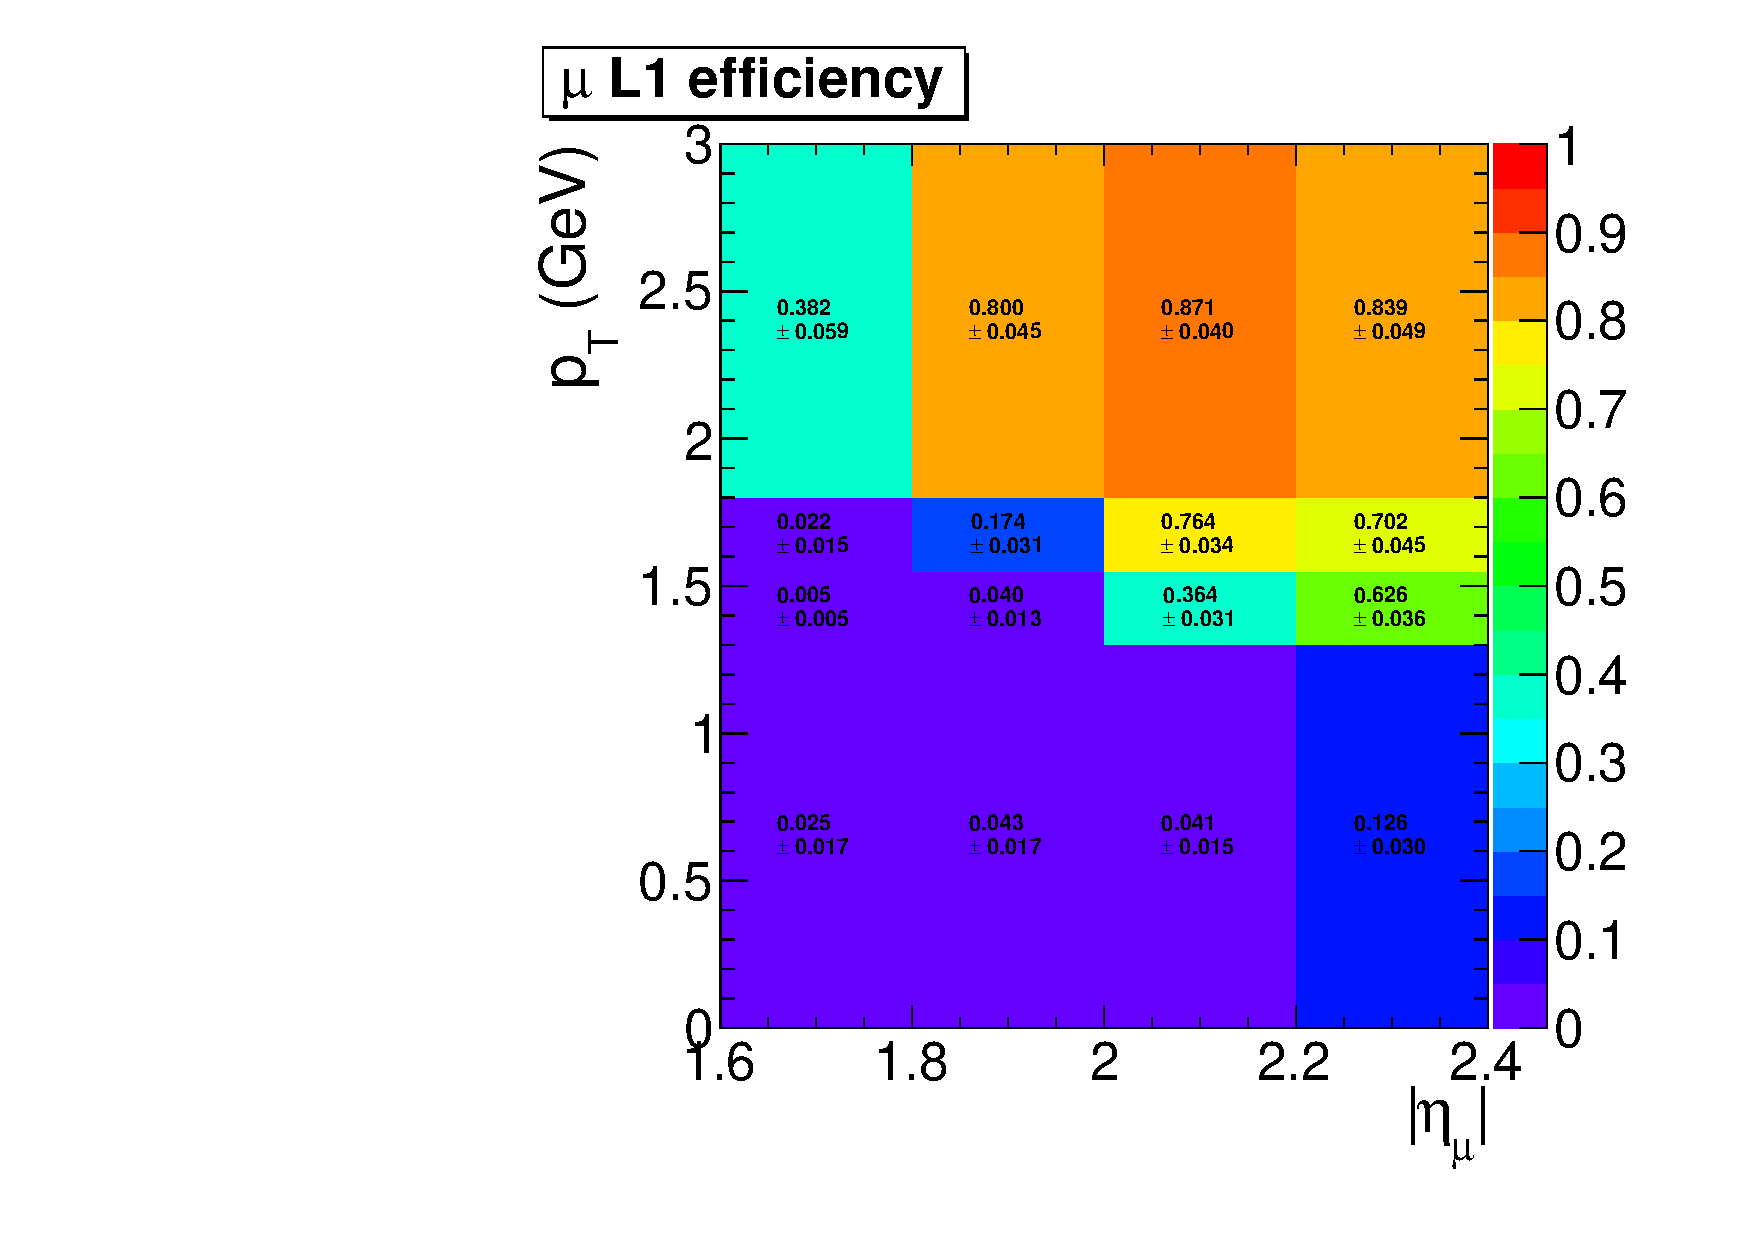
\includegraphics[width=.45\textwidth]{tNp/tnpCounting} &
          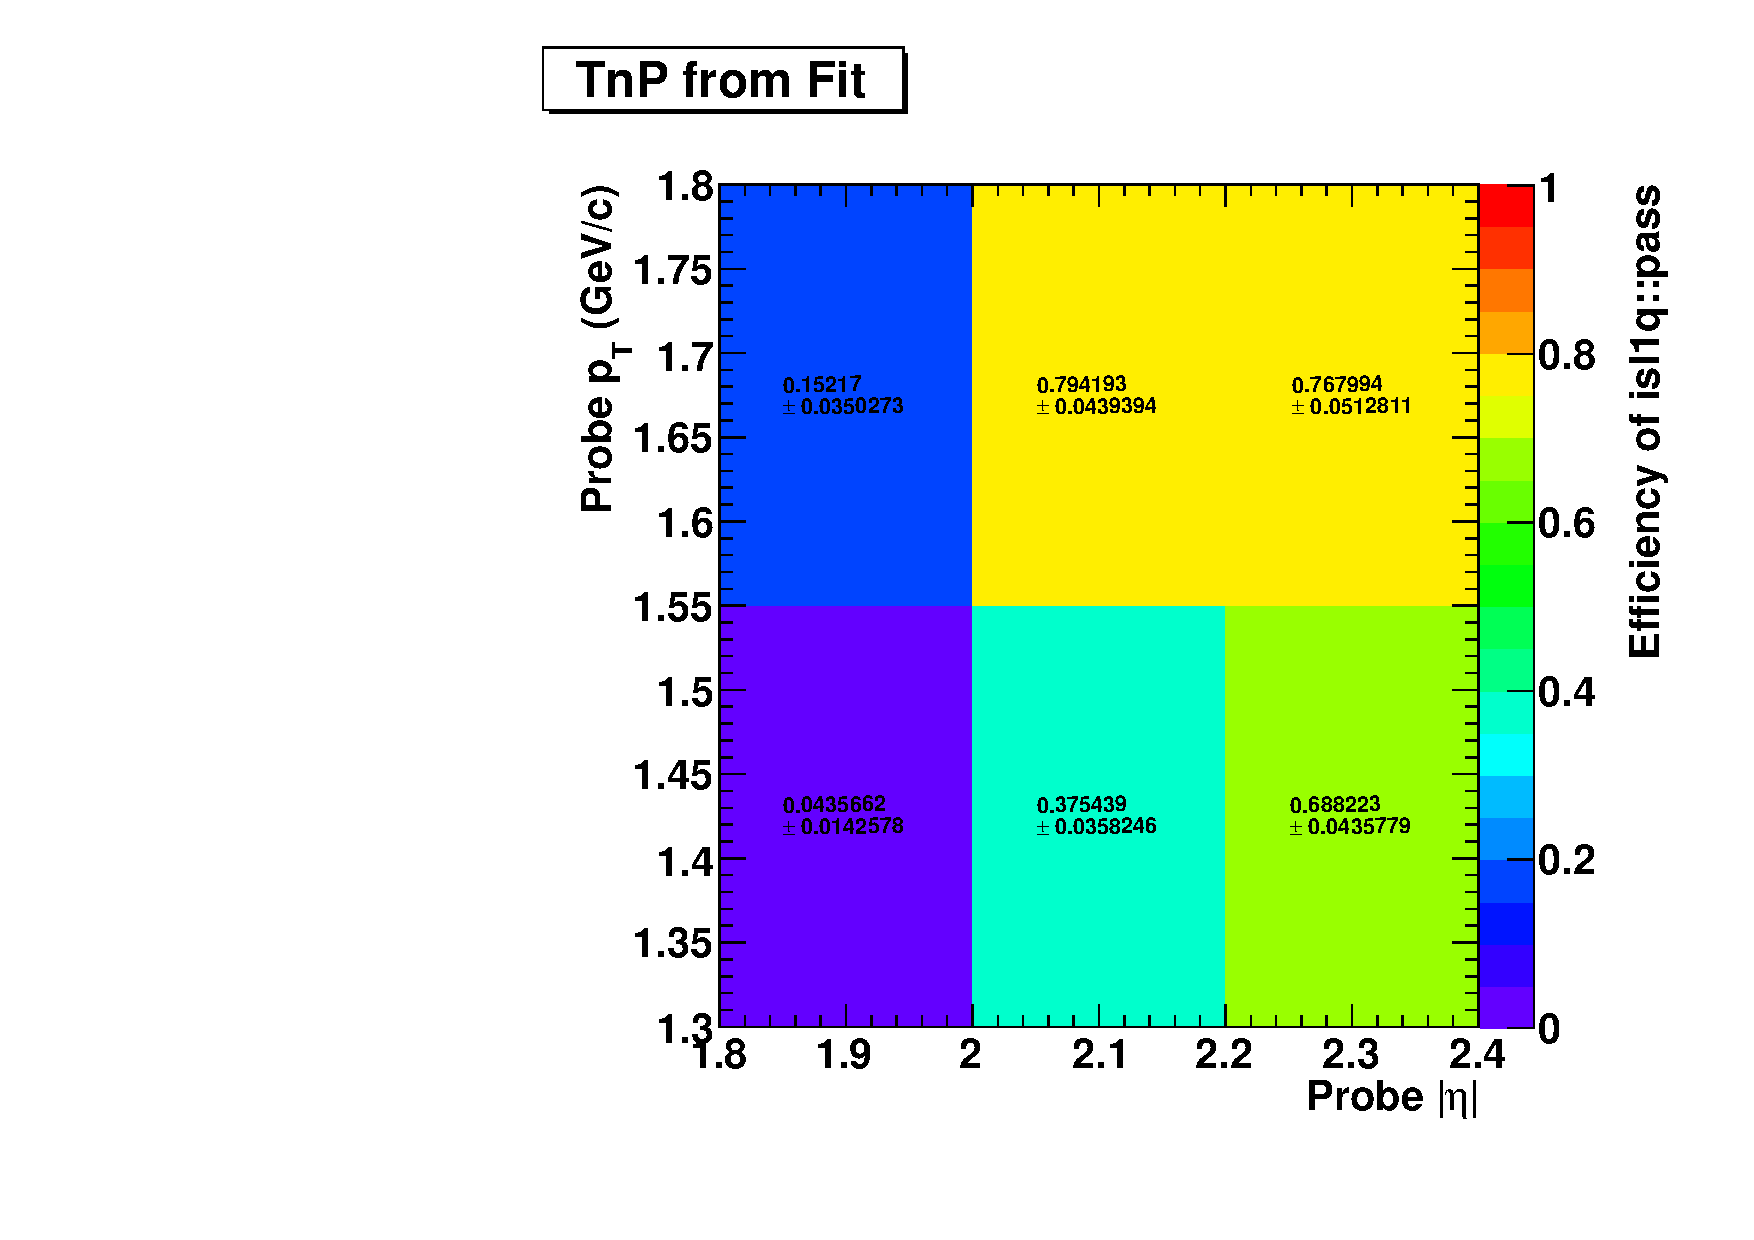
\includegraphics[width=.45\textwidth]{tNp/tnpFromFit}
        \end{array} $ 
        \caption{Tag and probe trigger efficiencies from counting (left) 
          compared to fitting (right)}
        \label{fig:tnpCntVFit}
      \end{figure}

      From Fig.~\ref{fig:tnpCntVFit} it is apparent that the choice of fit 
        function and therefore the amount of background from the mass side 
        bands is included in the signal measurement has very little effect on 
        the tag and probe efficiency measurement.
      The small effect of including the side bands is due to the side bands 
        being comprised mostly of photon-photon events.
      Because this background is neither decays from other particles like pions
        nor is it non-physical background like combinatorics, the efficiency
        for muons from the sidebands are nearly identical to \JPsi{} signal.
      The photon-photon process directly produces two muons just like the 
        \JPsi{}, therefore efficiency estimated from the side bands has 
        little effect on the measurement because of this similarity.
      The counting and fitting trigger efficiency measurements agree within 
        statistcal uncertainties, so this uncertianty was taken to be negliable.

    \subsection{MC vs Data compairson}
      \begin{figure}[h]
        \centering
        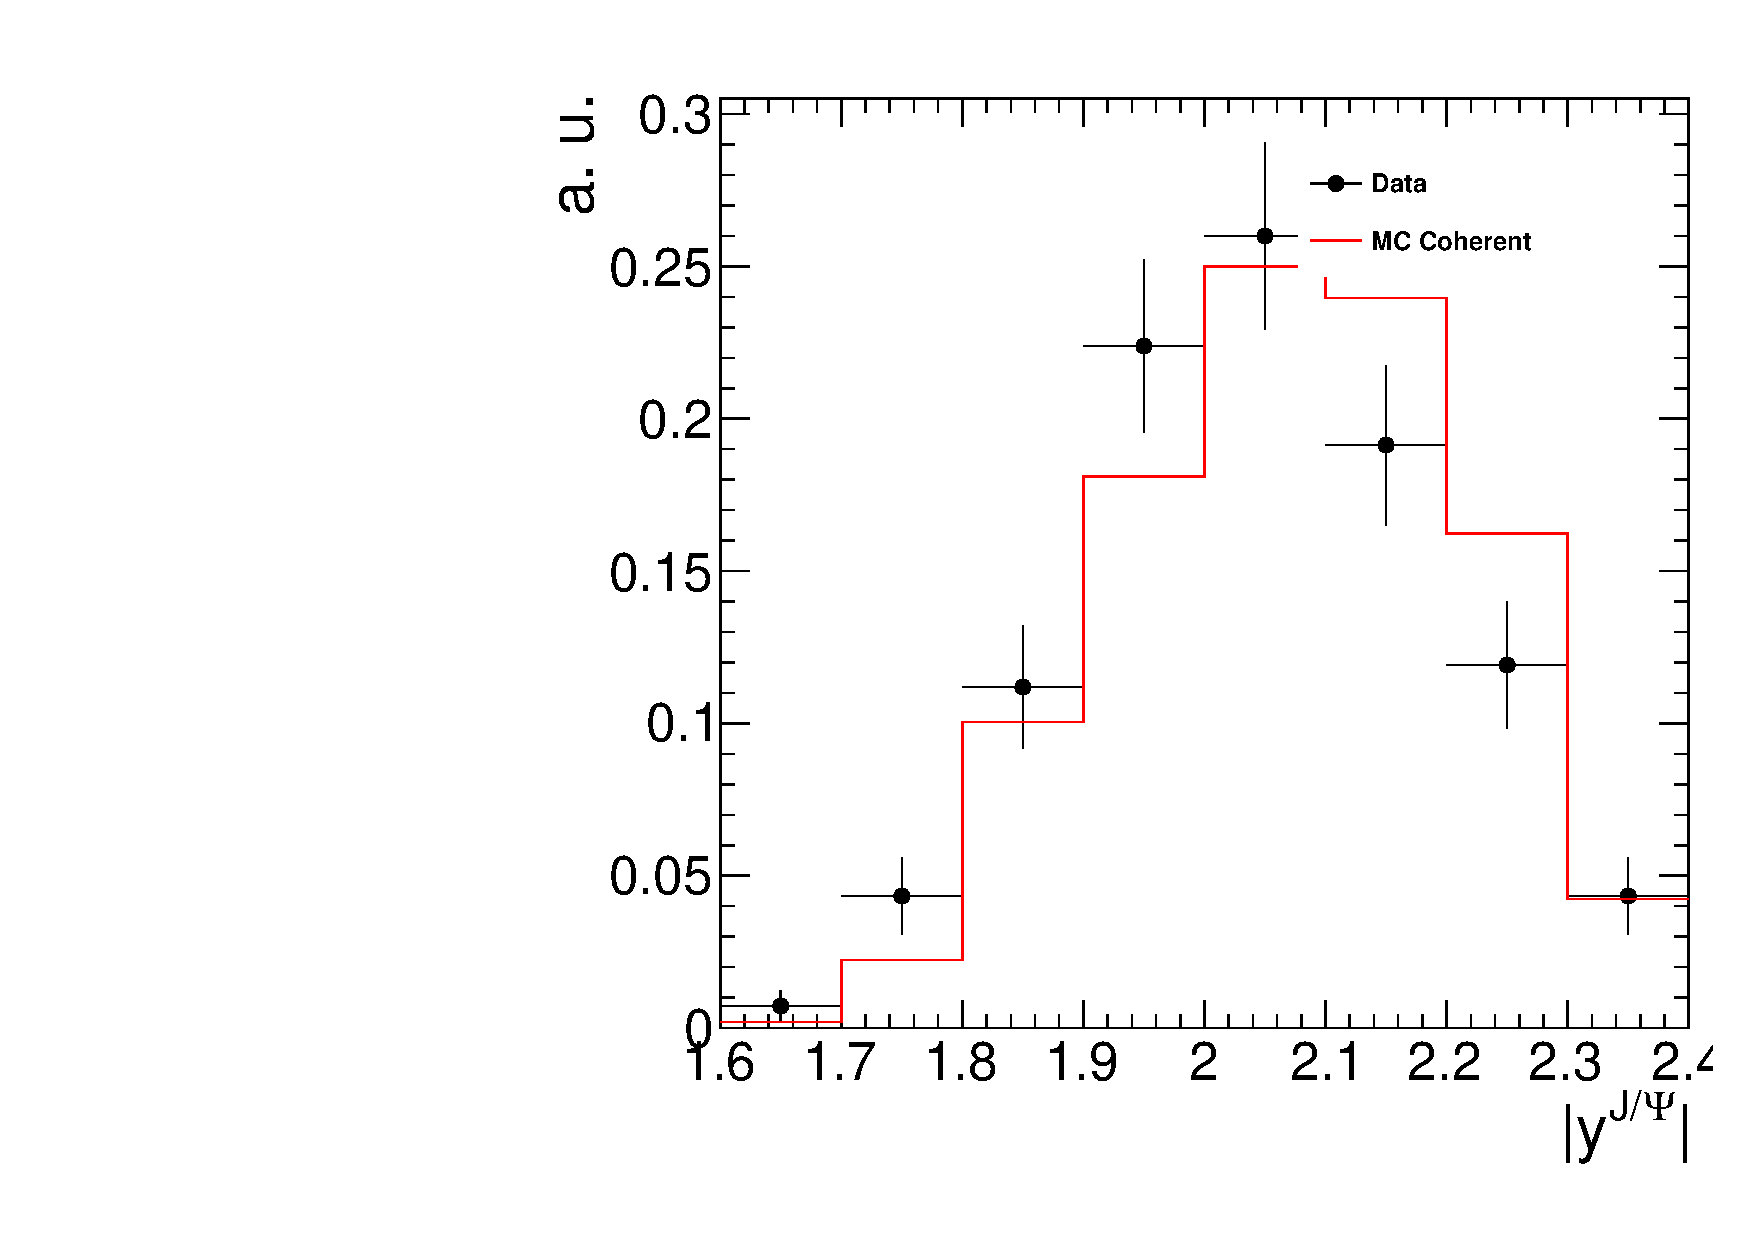
\includegraphics[width=0.5\textwidth]{jpsiMcComp/jpsiAbsRapCoherent}
        \caption{Comparison of the of the dimuon rapidity distributions between 
          coherent MC sample and Data.}
        \label{fig:jpsiAbsRapCoherent}
      \end{figure}
      \begin{figure}[h]
        \centering
        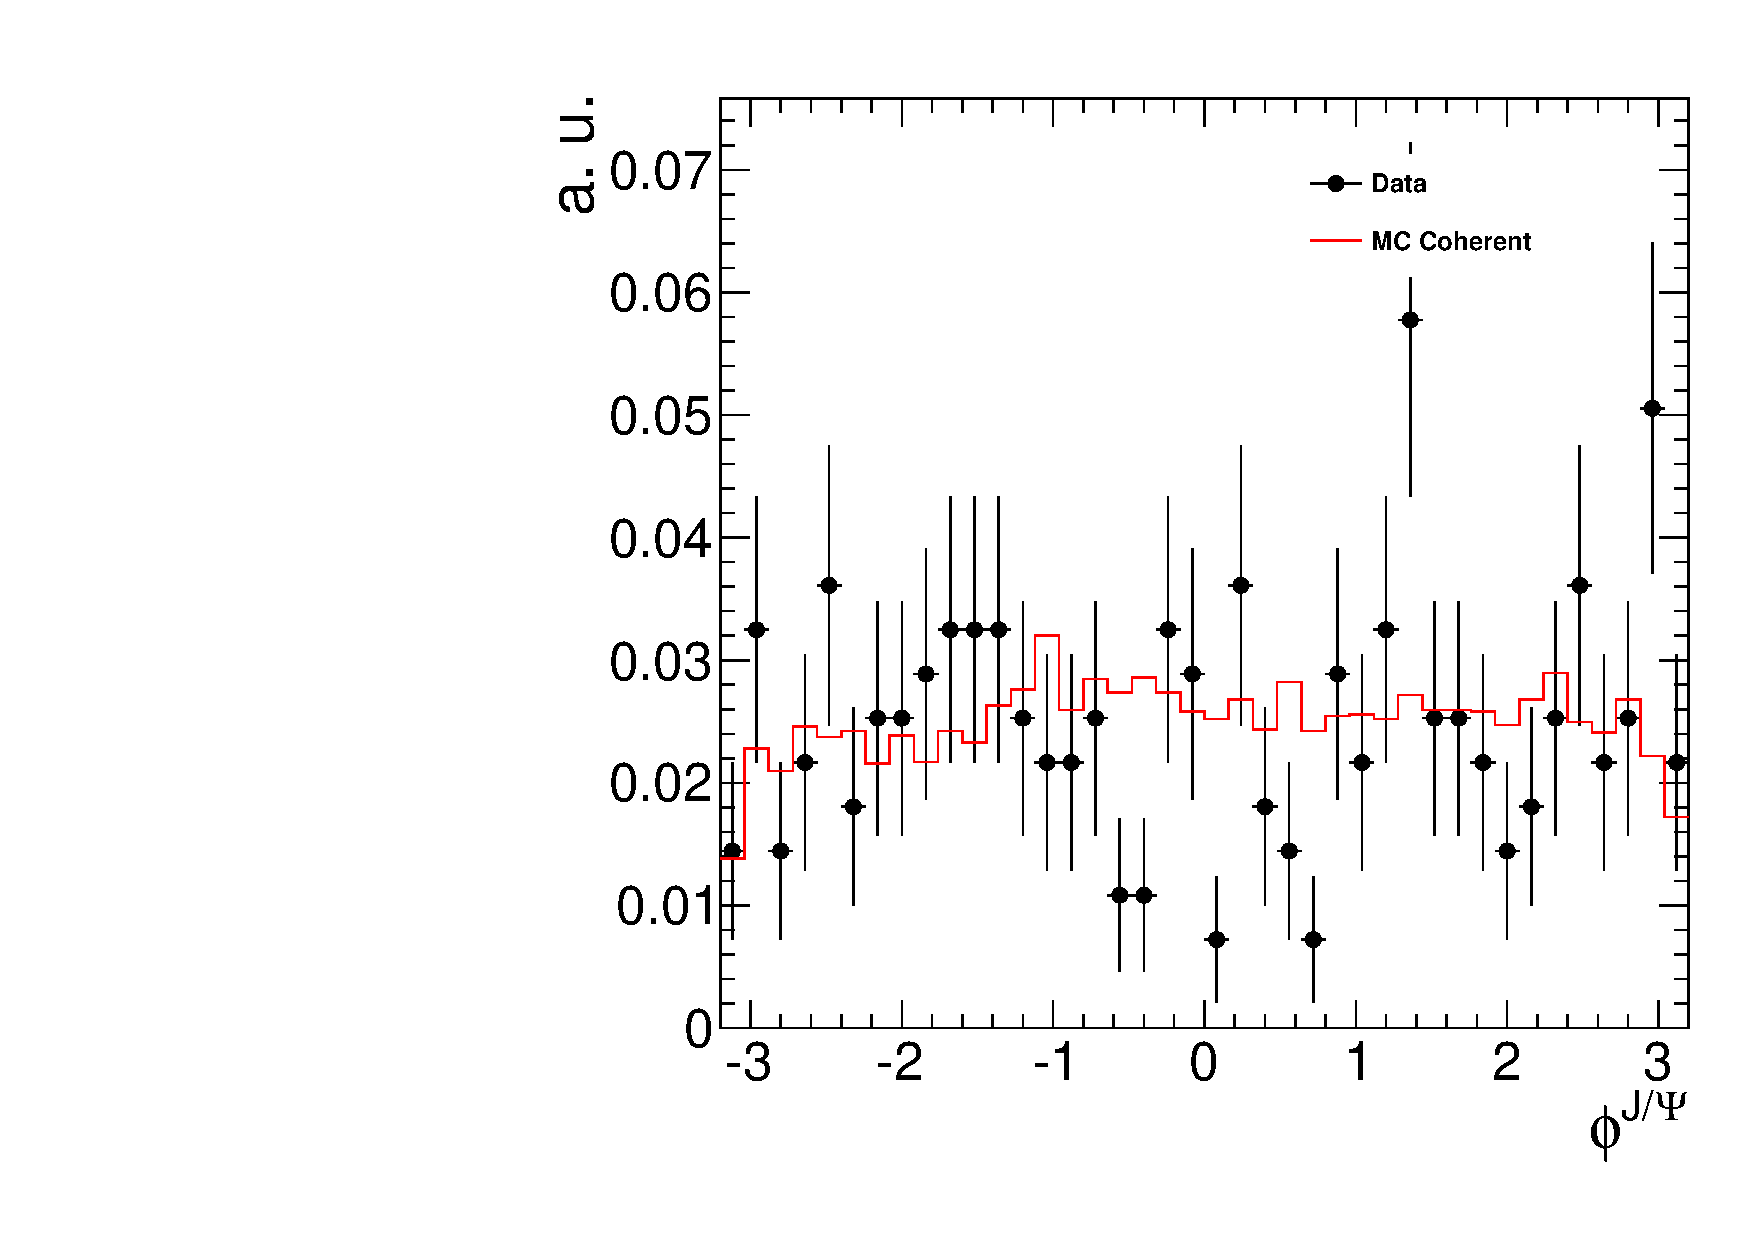
\includegraphics[width=0.5\textwidth]{jpsiMcComp/jpsiPhiCoherent}
        \caption{Comparison of the of the dimuon $\varphi$ distributions 
          between coherent MC sample and Data.}
        \label{fig:jpsiPhiCoherent}
      \end{figure}
      \begin{figure}[h]
        \centering
        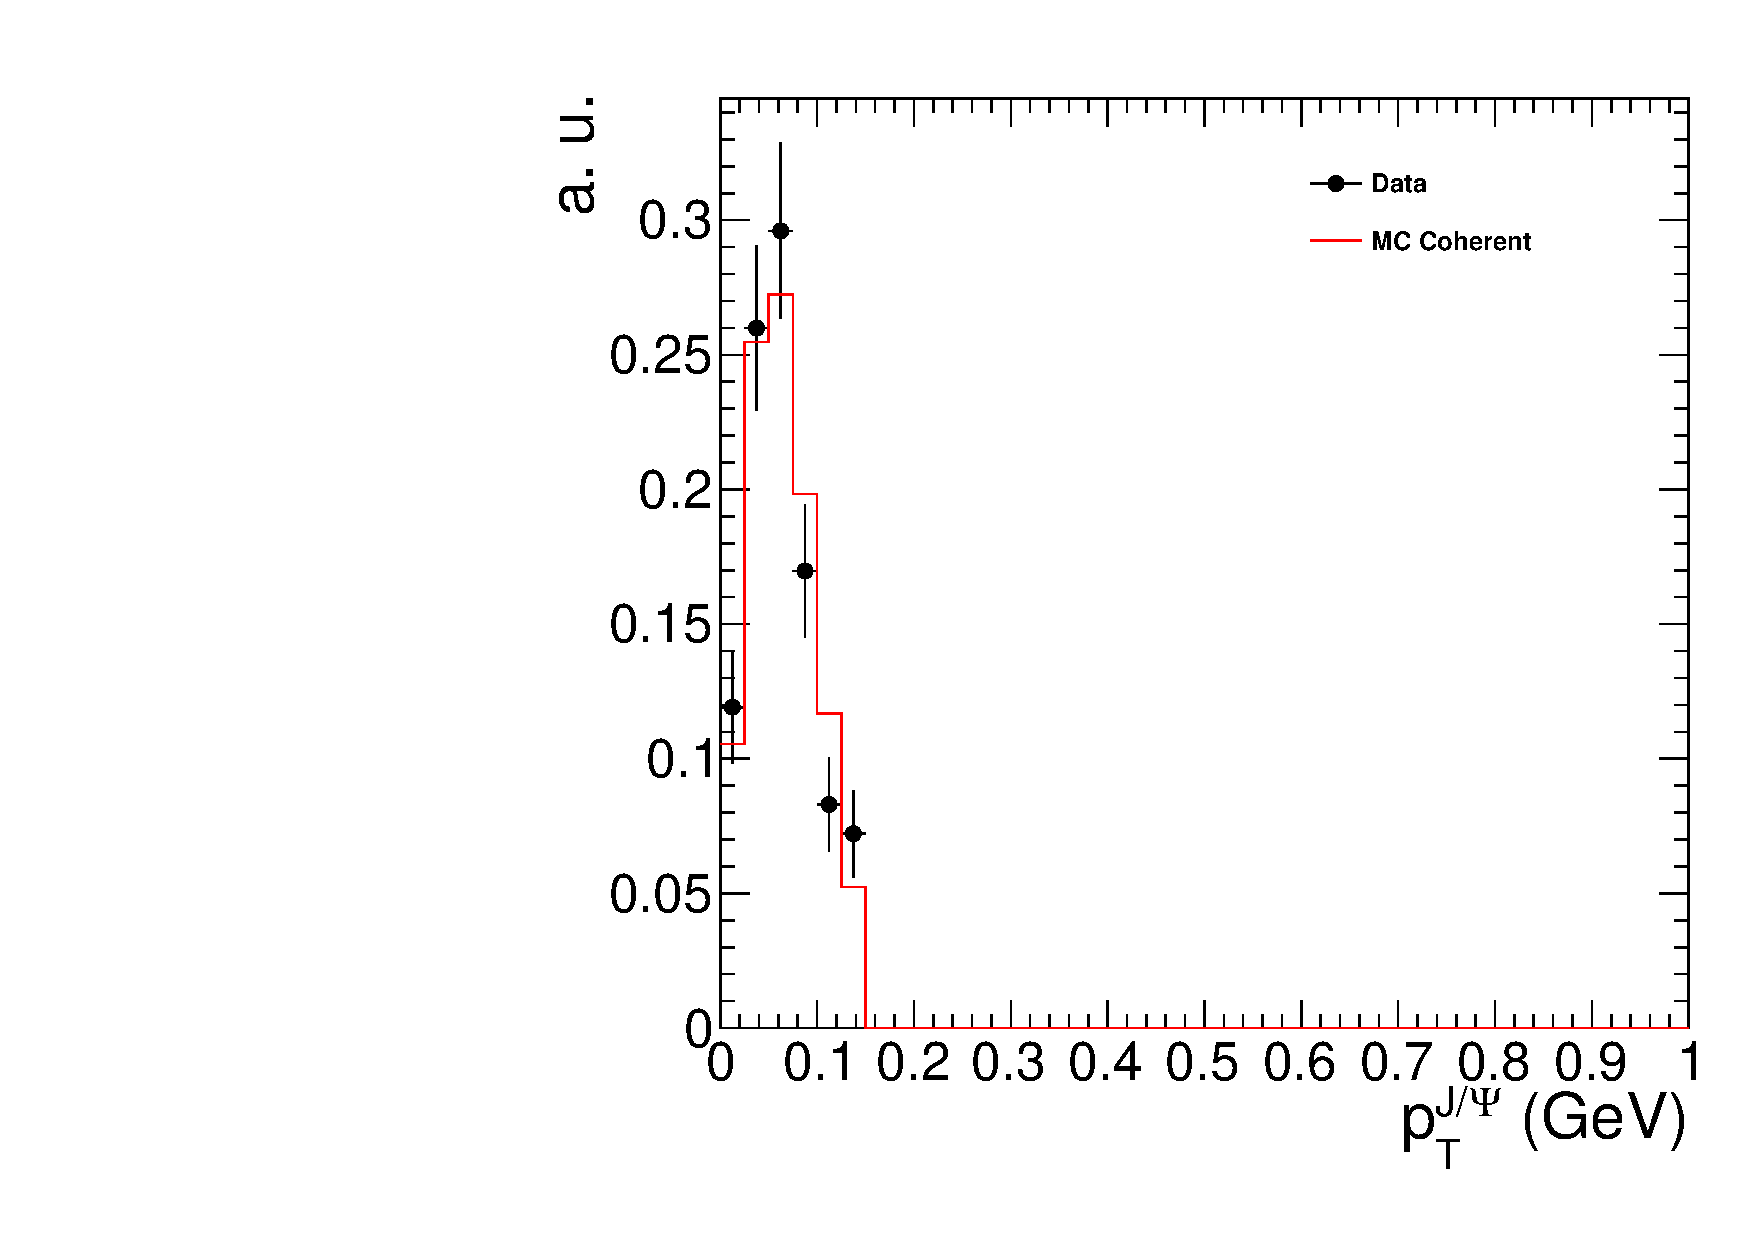
\includegraphics[width=0.5\textwidth]{jpsiMcComp/jpsiPtCoherent}
        \caption{Comparison of the of the dimuon \pt{} distributions 
          between coherent MC sample and Data.}
        \label{fig:jpsiPtCoherent}
      \end{figure}

